% Electro-optic measurement apparatus
    %% PDH servo
    %% Servo Parameters
	%%% Sensing S(f)
    	%%% Actuation A(f)
    	%%% Low Frequency Servo (Thermal Loop)
    	%%% OLG(f) 
    %% Longitudinal Pockels Cell mirror mount assembly
	%%% Modeling
    	%%% Voltage drive electronics
    %% Servo Overview
    %% Calibration

% Results
    %% Mounting Strategies
	%%% Assembly 1
    	%%% Assembly 2
    	%%% Assembly 3 (MACOR mount)
    	%%% Acousto-optical coupling

% Conclusion

\section{Electro-optic measurement apparatus}\label{tanioka2022}
%In seeking a calibrated estimate of the electro-optic effect for the $\gaas$/$\algaas$ mirror coating stack, we sought to drive an electro-optic response of a mirror sample from Thorlab's crystalline mirror coatings division placed within a custom longitudinal Pockels cell mirror mount. The assembly, with the installed sample, assumed the end mirror position within a two mirror Fabry-P\'erot cavity, while resonance of a circulating Nd:YAG 1064nm carrier beam was held by a Pound-Drever-Hall servo. As seen in the prior section, the size of the imparted phase noise for currently existing gravitational wave detector configurations is estimated to be small but notable. Investigation through measurement of said effect requires detection methods with sufficient sensitivity for the differential phase noise imparted by the effect. Details and specifications of the detection schema are discussed along with relevant measurements and results. 

In order to experimentally investigate the EO effect in $\gaas$ / $\algaas$ coatings, we developed an optical setup using a Fabry-P\'erot cavity. \autoref{fig:simpschema} shows the schematic of the experimental setup. Parameters of this setup are listed in \autoref{table:cav_params}. The Fabry-P\'erot cavity is composed of two high-reflectivity mirrors -- an amorphous coating front mirror and $\gaas$/$\algaas$ coating with the same composition used in \autoref{algaas_numericalestimate}, transferred to a planar super-polished fused silica substrate. 

\begin{figure}[H]
    \centering
	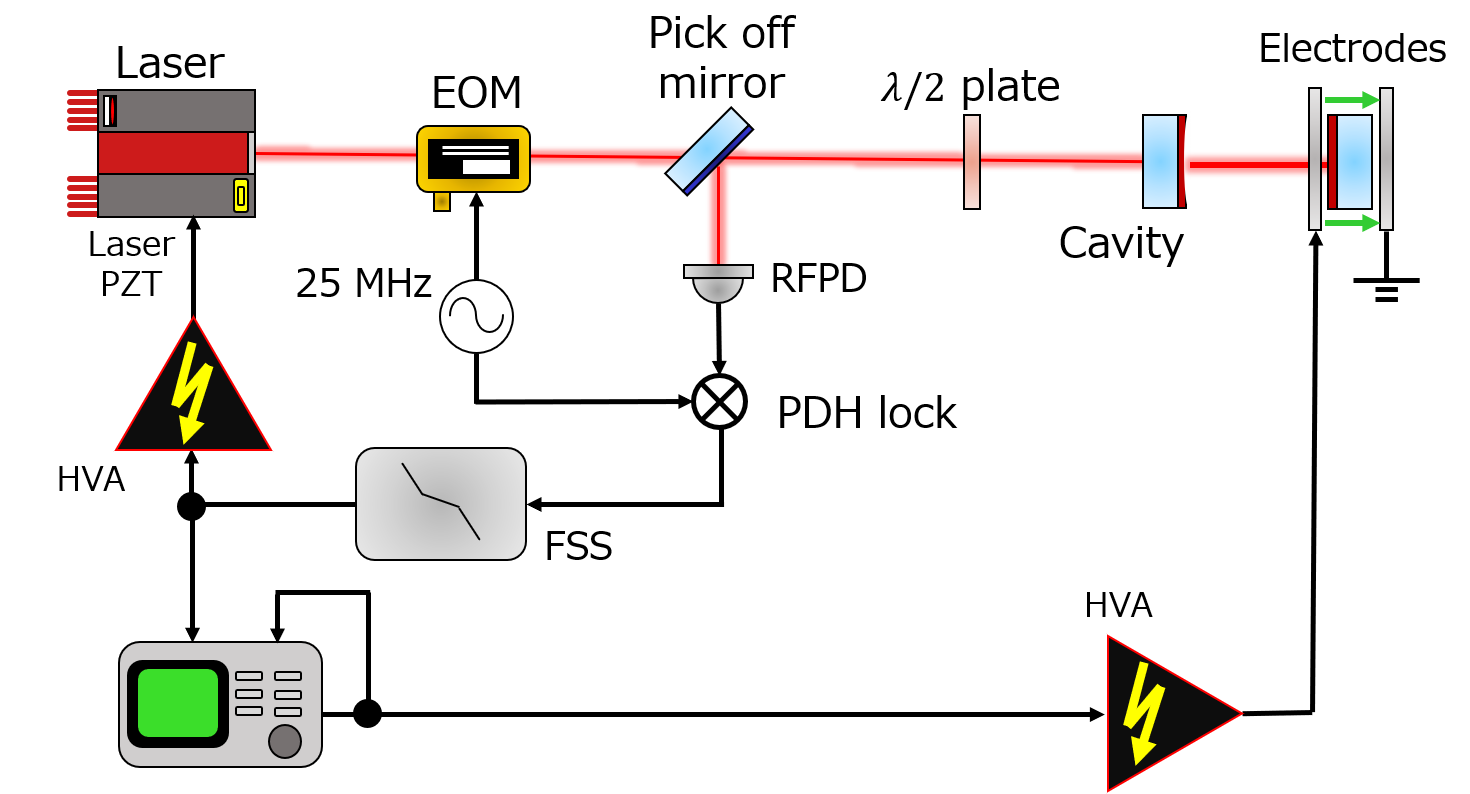
\includegraphics[width=\textwidth]{tanioka_2022/setup.png}
	\caption{A simplified and modular schematic of the PDH servo used along with an electrostatic drive mount design comprised of a disk capacitor sandwiching the HR AlGaAs sample, a high voltage amplifier, and a signal / network analyzer.}
\label{fig:simpschema}
\end{figure}
 Measurability of the electro-optic effect is contingent upon two initial design criteria: the sensitivity of the optical plant to be implemented in the PDH servo, and the maximum achievable electric field strength along the beam axis ($|E_z|_\mathrm{max}$). 

\subsection{Servo Parameters}
The quantity we are attempting to measure is a differential length coupling on the order of $3.3 \times 10^{-18}$ [m/(V/m)], motivating a short cavity design as the relative differential length (phase) change scales with the sensitivity \autoref{eq:cavlf}. Considerations of the lab mirror inventory and mode matching critera lead us to two candidate plano-concave (ROC = 0.333m) HR IBS coated sample input couplers; one from CVI Melles-Griot and another from ATFilms. When paired with the plano-plano $\gaas$/$\algaas$  mirror from the Crystalline Mirror Solutions (CMS) division of Thorlabs, designed cavity length was 0.105 m.

%\begin{figure}[H]
%\begin{center}
%\includegraphics[width=.80\textwidth]{ALGAAS/opt_layout_b.pdf}
%\end{center}
%\caption{\textcolor{red}{Final figure still pending} Detailed optical schema of the experiment. Components highlighted in magenta indicate laser back-reflection protection and output power control. All optics highlighted in PURPLE indicate their function as alignment and mode matching for locking to a triangular ALIGO PMC \textbf{Multiple citations (DCC doc / Fabian's experiment / Erik's experiment)}. Optics highlighted in YELLOW indicate function for alignment and mode matching to the experimental cavity utilizing the HR $\gaas$/$\algaas$ coated mirror sample. Beam profiling to the sample cavity is indicated. For the sake of the numerous mounting strategies tried, the longitudinal pockels cell mirror mount is kept general with the pictured mirror between two disk capacitors}
%\label{fig:expoptical_layout}
%\end{figure}
%%FIGURE: Servo diagram
%%CAPTION: A simplified diagram of the servo used. The highlighted regions of the schematic are intended to provide a modular view; highlighting the components required for the PDH servo to operate.}

The implemented servo design uses a light source from a Mephisto 2000 NE Nd:YAG laser with a 25 MHz phase modulation from a New Focus Model 4003 IR resonant phase modulator. As indicated in the figure above, the electronics chain can be decomposed into two primary filter components: $S(f)$ and $A(f)$. The following table provides a summary with relevant experiment parameters:

\begin{table}[h!]
\caption{Parameters of experimental setup.}
\centering 
\begin{tabular}{lcc}
    \hline \hline
    Symbol & Description & Value \\
    \hline
    $\lambda$ & Laser wavelength & $1064 \, \mathrm{nm}$ \\
    $L$ & Cavity length & $0.105\, \mathrm{m}$ \\
    $T_i$ & Power transmissivity of input mirror & $\sim0.5\%$ \\
    $T_e$ & Power transmissivity of output mirror & $\sim10\, \mathrm{ppm}$ \\
    $f_c$ & Cavity pole frequency & $\sim600\, \mathrm{kHz}$ \\
    $x$ & Aluminum alloying fraction & 0.92 \\
    $d_{\mathrm{H}}$ & Thickness of $\mathrm{GaAs}$ & $76.43\, \mathrm{nm}$ \\
    $n_{\mathrm{H}}$ & Refractive index of $\mathrm{GaAs}$ & $3.48$ \\
    $d_{\mathrm{L}}$ & Thickness of $\mathrm{Al_{0.92}Ga_{0.08}As}$ & $89.35\, \mathrm{nm}$ \\
    $n_{\mathrm{L}}$ & Refractive index of $\mathrm{Al_{0.92}Ga_{0.08}As}$ & $2.98$ \\
    \hline \hline
\end{tabular} \label{table:cav_params}
\end{table}

The laser frequency is locked to the cavity length using the aformentioned Pound-Derver-Hall technique. The extracted error signal is then filtered by the Sensing chain (S(f)) before being passed to the Actuation chain (A(f)). When the laser is locked to the in-air cavity, the fluctuations of the laser frequency ($\Delta f$) obey \autoref{eq:cavlf}. 

\subsubsection{Sensing S(f)}
Sensing electronics are composed of a single element photodiode mounted to a tranimpedance amplifier circuit, splitting photocurrent to DC and RF filter chains. The RF path is within the feedback electronics chain and constructed to boost the RF signal prior to being passed to a frequency stabilization servo (FSS) \autoref{fig:fss_tf} where it is demodulated by mixing the 25 MHz oscillator phased with variable cable length. Once demodulated, the measured beat signal while sweeping through resonance generates the PDH error signal profiles \autoref{fig:pdherr}, and \autoref{appendix:laser_sweep}.

\begin{landscape}
    \section{FSS transfer function (LTSPICE)}\label{fig:fss_tf}
\begin{figure}[H]
  \begin{center}
    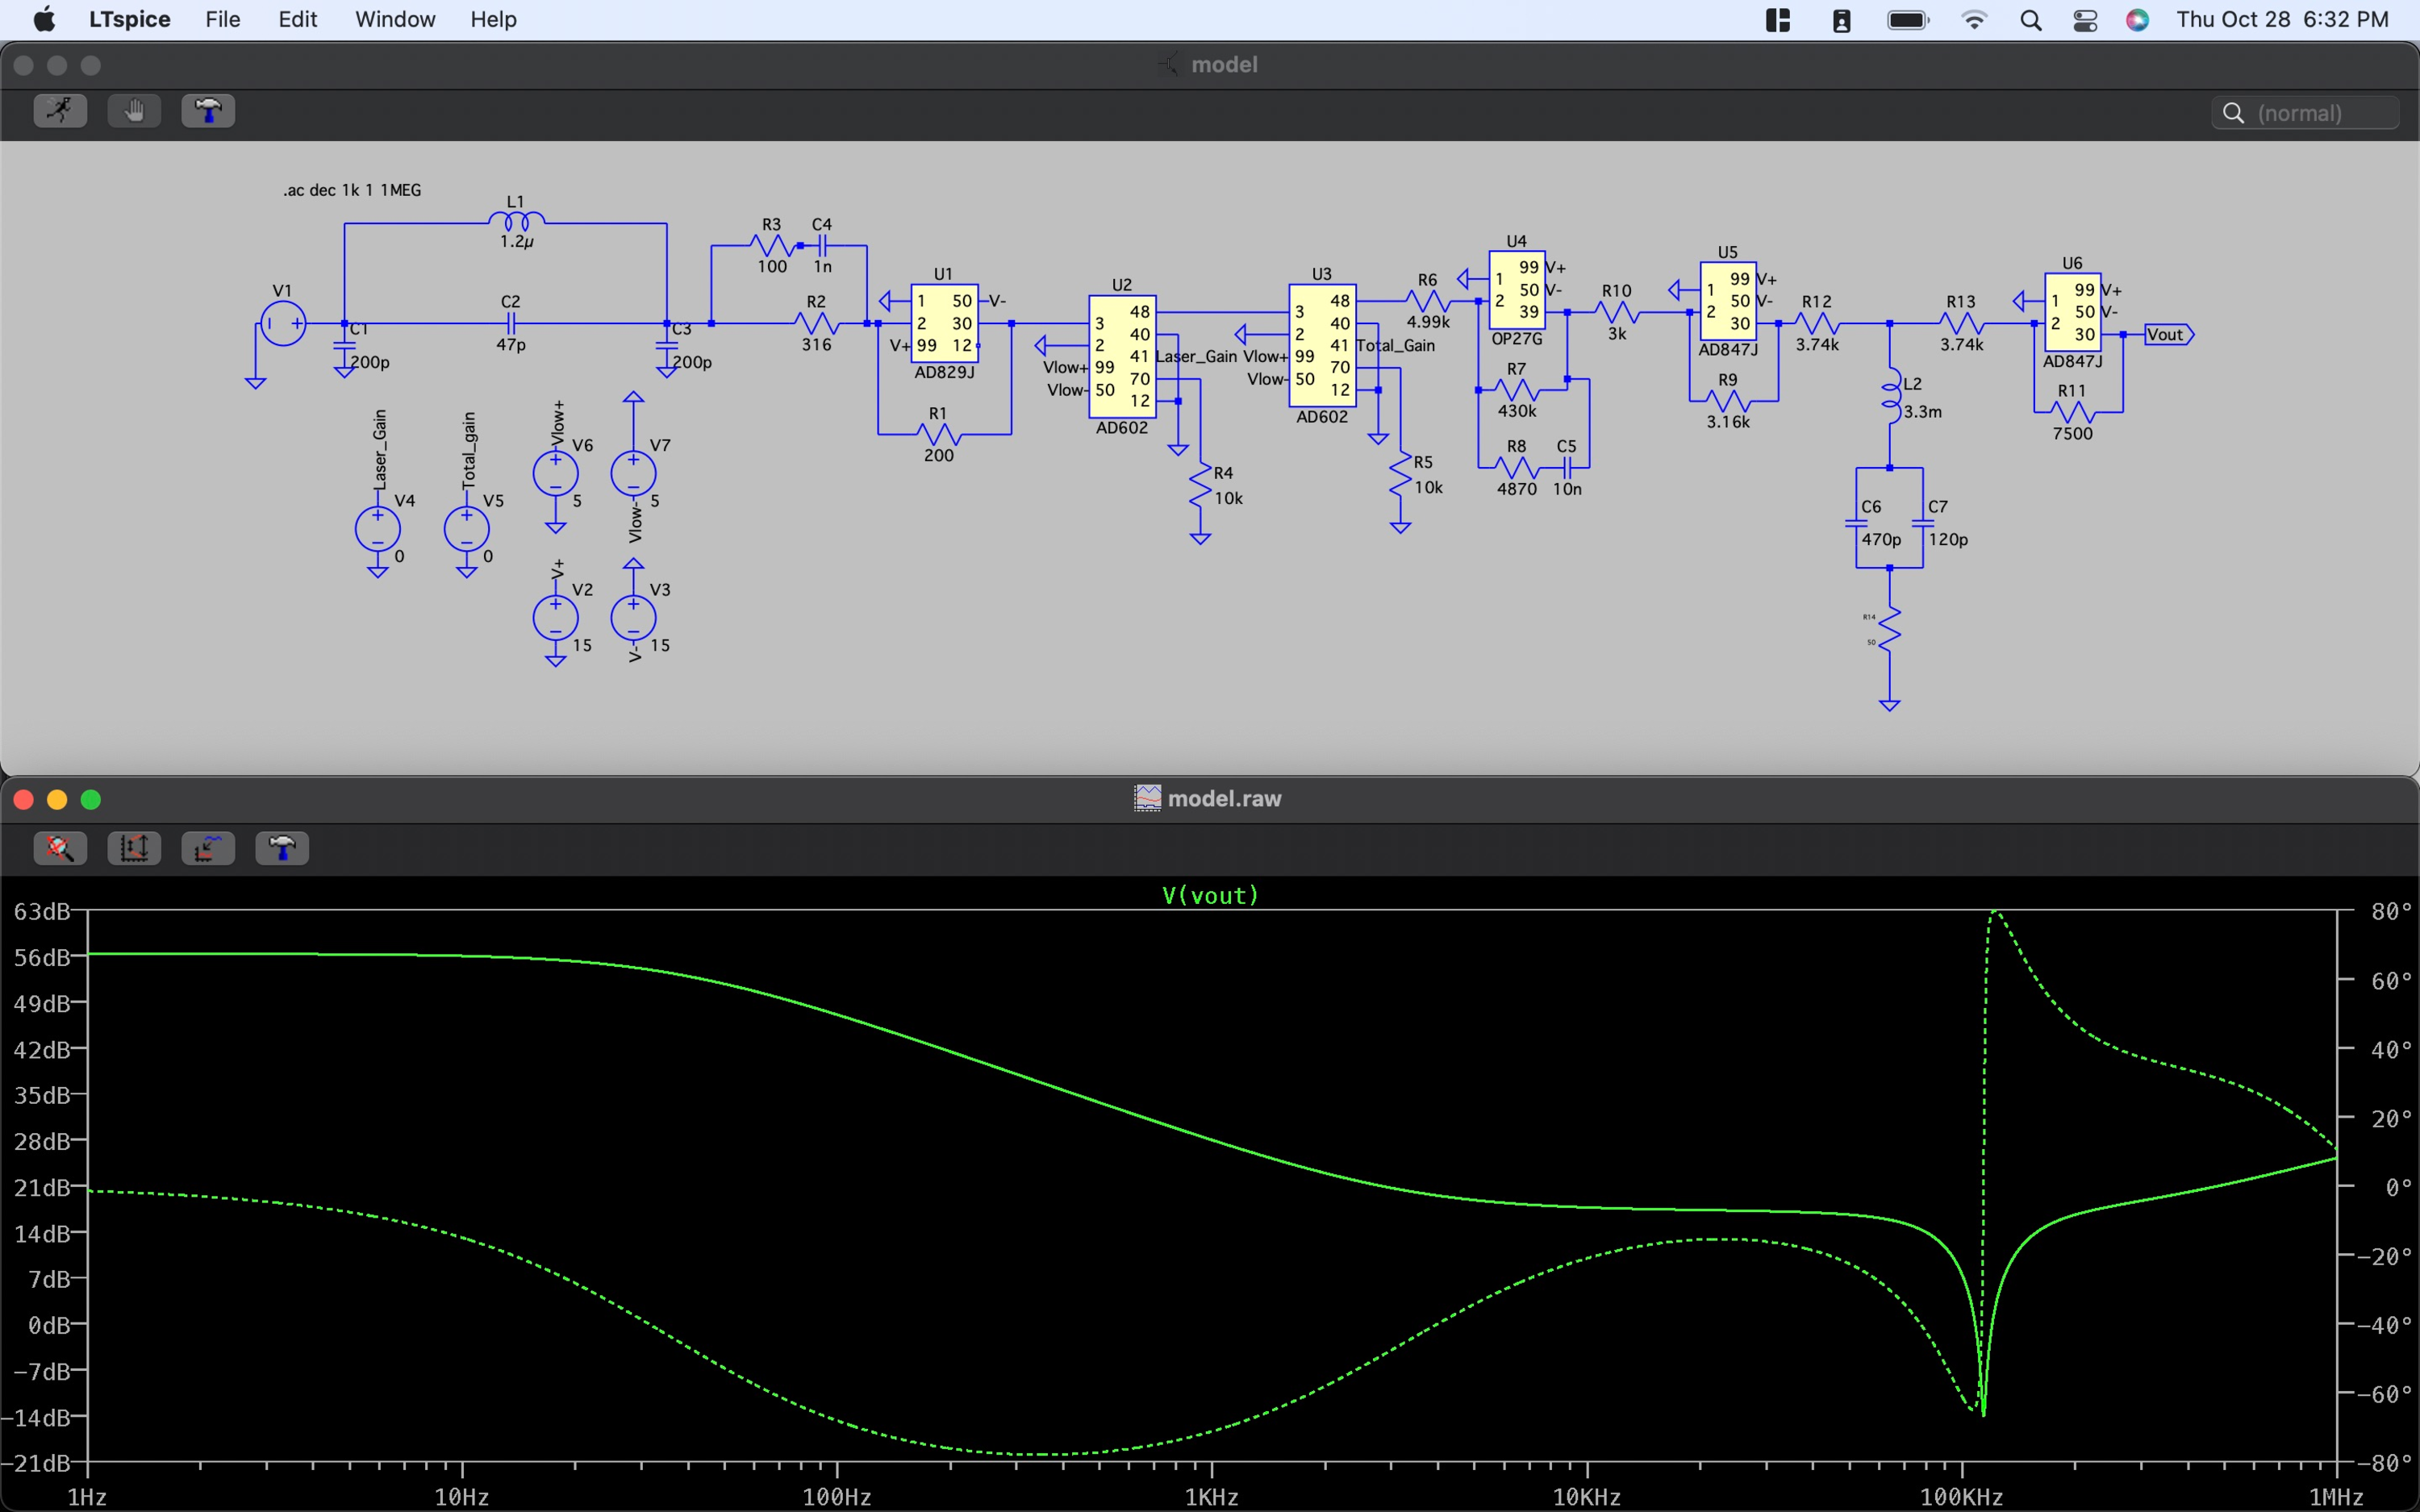
\includegraphics[width=1.33\textwidth]{figs/ALGAAS/tfs/spice_FSS_tf.pdf}
    \caption{The FSS frequency response simulated in LTspice}
  \end{center}
  \label{fig:spiceFSS}
\end{figure}
\end{landscape}


\subsubsection{Actuation A(f)}
The actuation portion of the loop amplifies the FSS output with a single I/O channel of the SVR 350-3 BIP High Voltage Amplifier \footnote{HVA transfer function \autoref{appendix:hva_tfs}} from Piezomechanik GmbH with a custom pomona box fed back to the input ~\cite{sugwglog:412} . The Mephisto 2220 laser cavity PZT actuator follows immediately after with a measured actuation factor of 1.7 [MHz] / [V].


\subsubsection{Loop Gain G(f)}
\begin{figure}[H]
  \begin{center}
    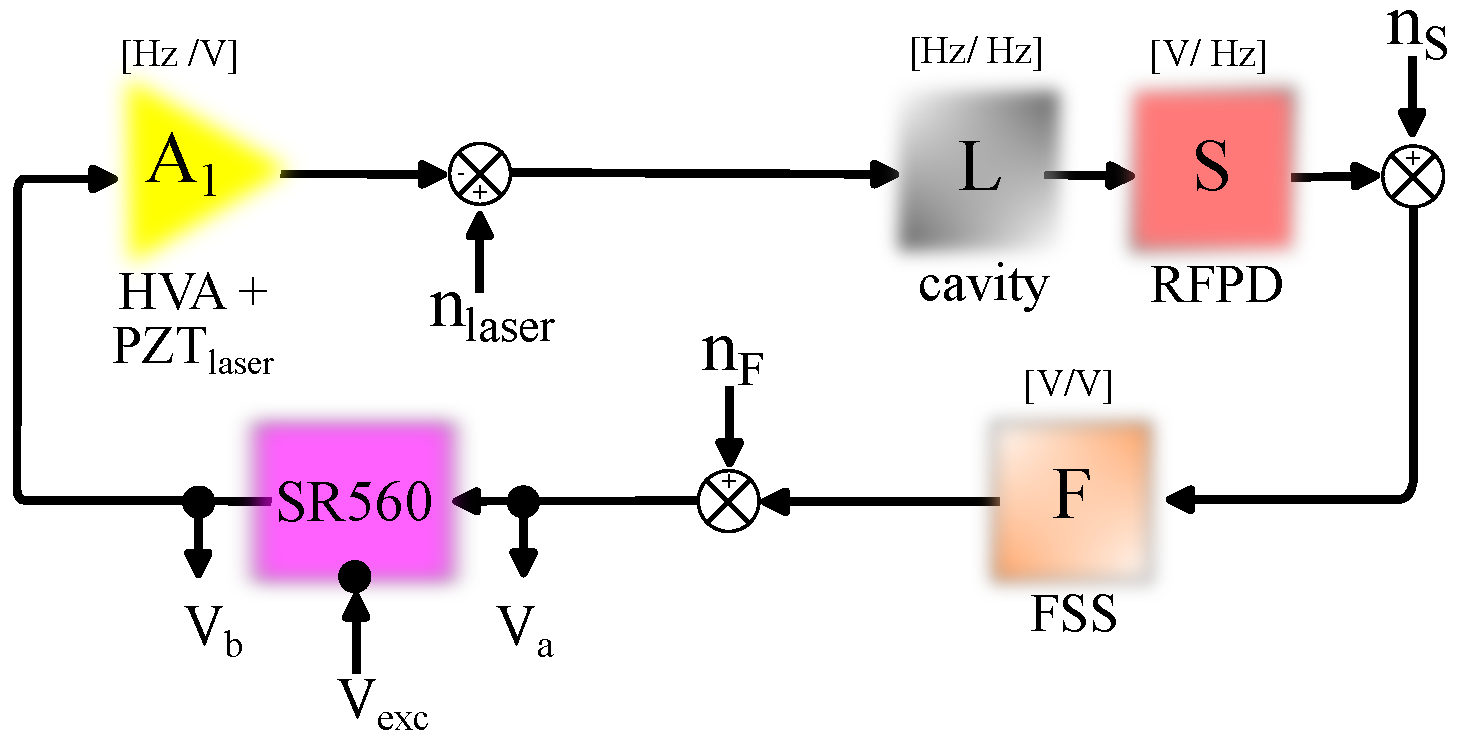
\includegraphics[width=\textwidth]{figs/ALGAAS/olg_meas_diagram.pdf}
    \caption{Open loop gain measurement diagram}
  \end{center}
  \label{fig:OLGmath}
\end{figure}

\begin{equation}
    \mathrm{V}_\mathrm{b} = (\mathrm{V}_\mathrm{exc}+n) + H(\mathrm{V}_\mathrm{exc}+n) + H^2 (\mathrm{V}_\mathrm{exc}+n) + \mathrm{H.O.T.s} = \frac{\mathrm{V}_\mathrm{exc} + n}{1-H}
\end{equation}

\begin{equation}
    \mathrm{V}_\mathrm{a} = H\cdot \mathrm{V}_\mathrm{exc} + H^2\mathrm{V}_\mathrm{exc} + H^3\mathrm{V}_\mathrm{exc} + \mathrm{H.O.T.s}  = \frac{H\mathrm{V}_\mathrm{exc}}{1-H}
\end{equation}

We take the transfer function measurement $\zeta$:

\begin{equation}
    \zeta = \frac{\mathrm{V}_\mathrm{a}}{\mathrm{V}_\mathrm{b}} = \frac{H \cdot \mathrm{V}_\mathrm{exc}/(1-H)}{(\mathrm{V}_\mathrm{exc}+n)/(1-H)}
\end{equation}

Assuming the excitation is appreciably larger than the noise ($e>>n$):

\begin{equation}
\zeta \approx H
\end{equation}

Isn't quite $\mathrm{A}(f)*\mathrm{S}(f)$ as stated. Doesn't entirely account for the optical plant.
How the measurement is taken (important to take between installations to account for the changes in the optical plant)~\cite{sugwglog:831}.

\begin{figure}[H]
\begin{center}
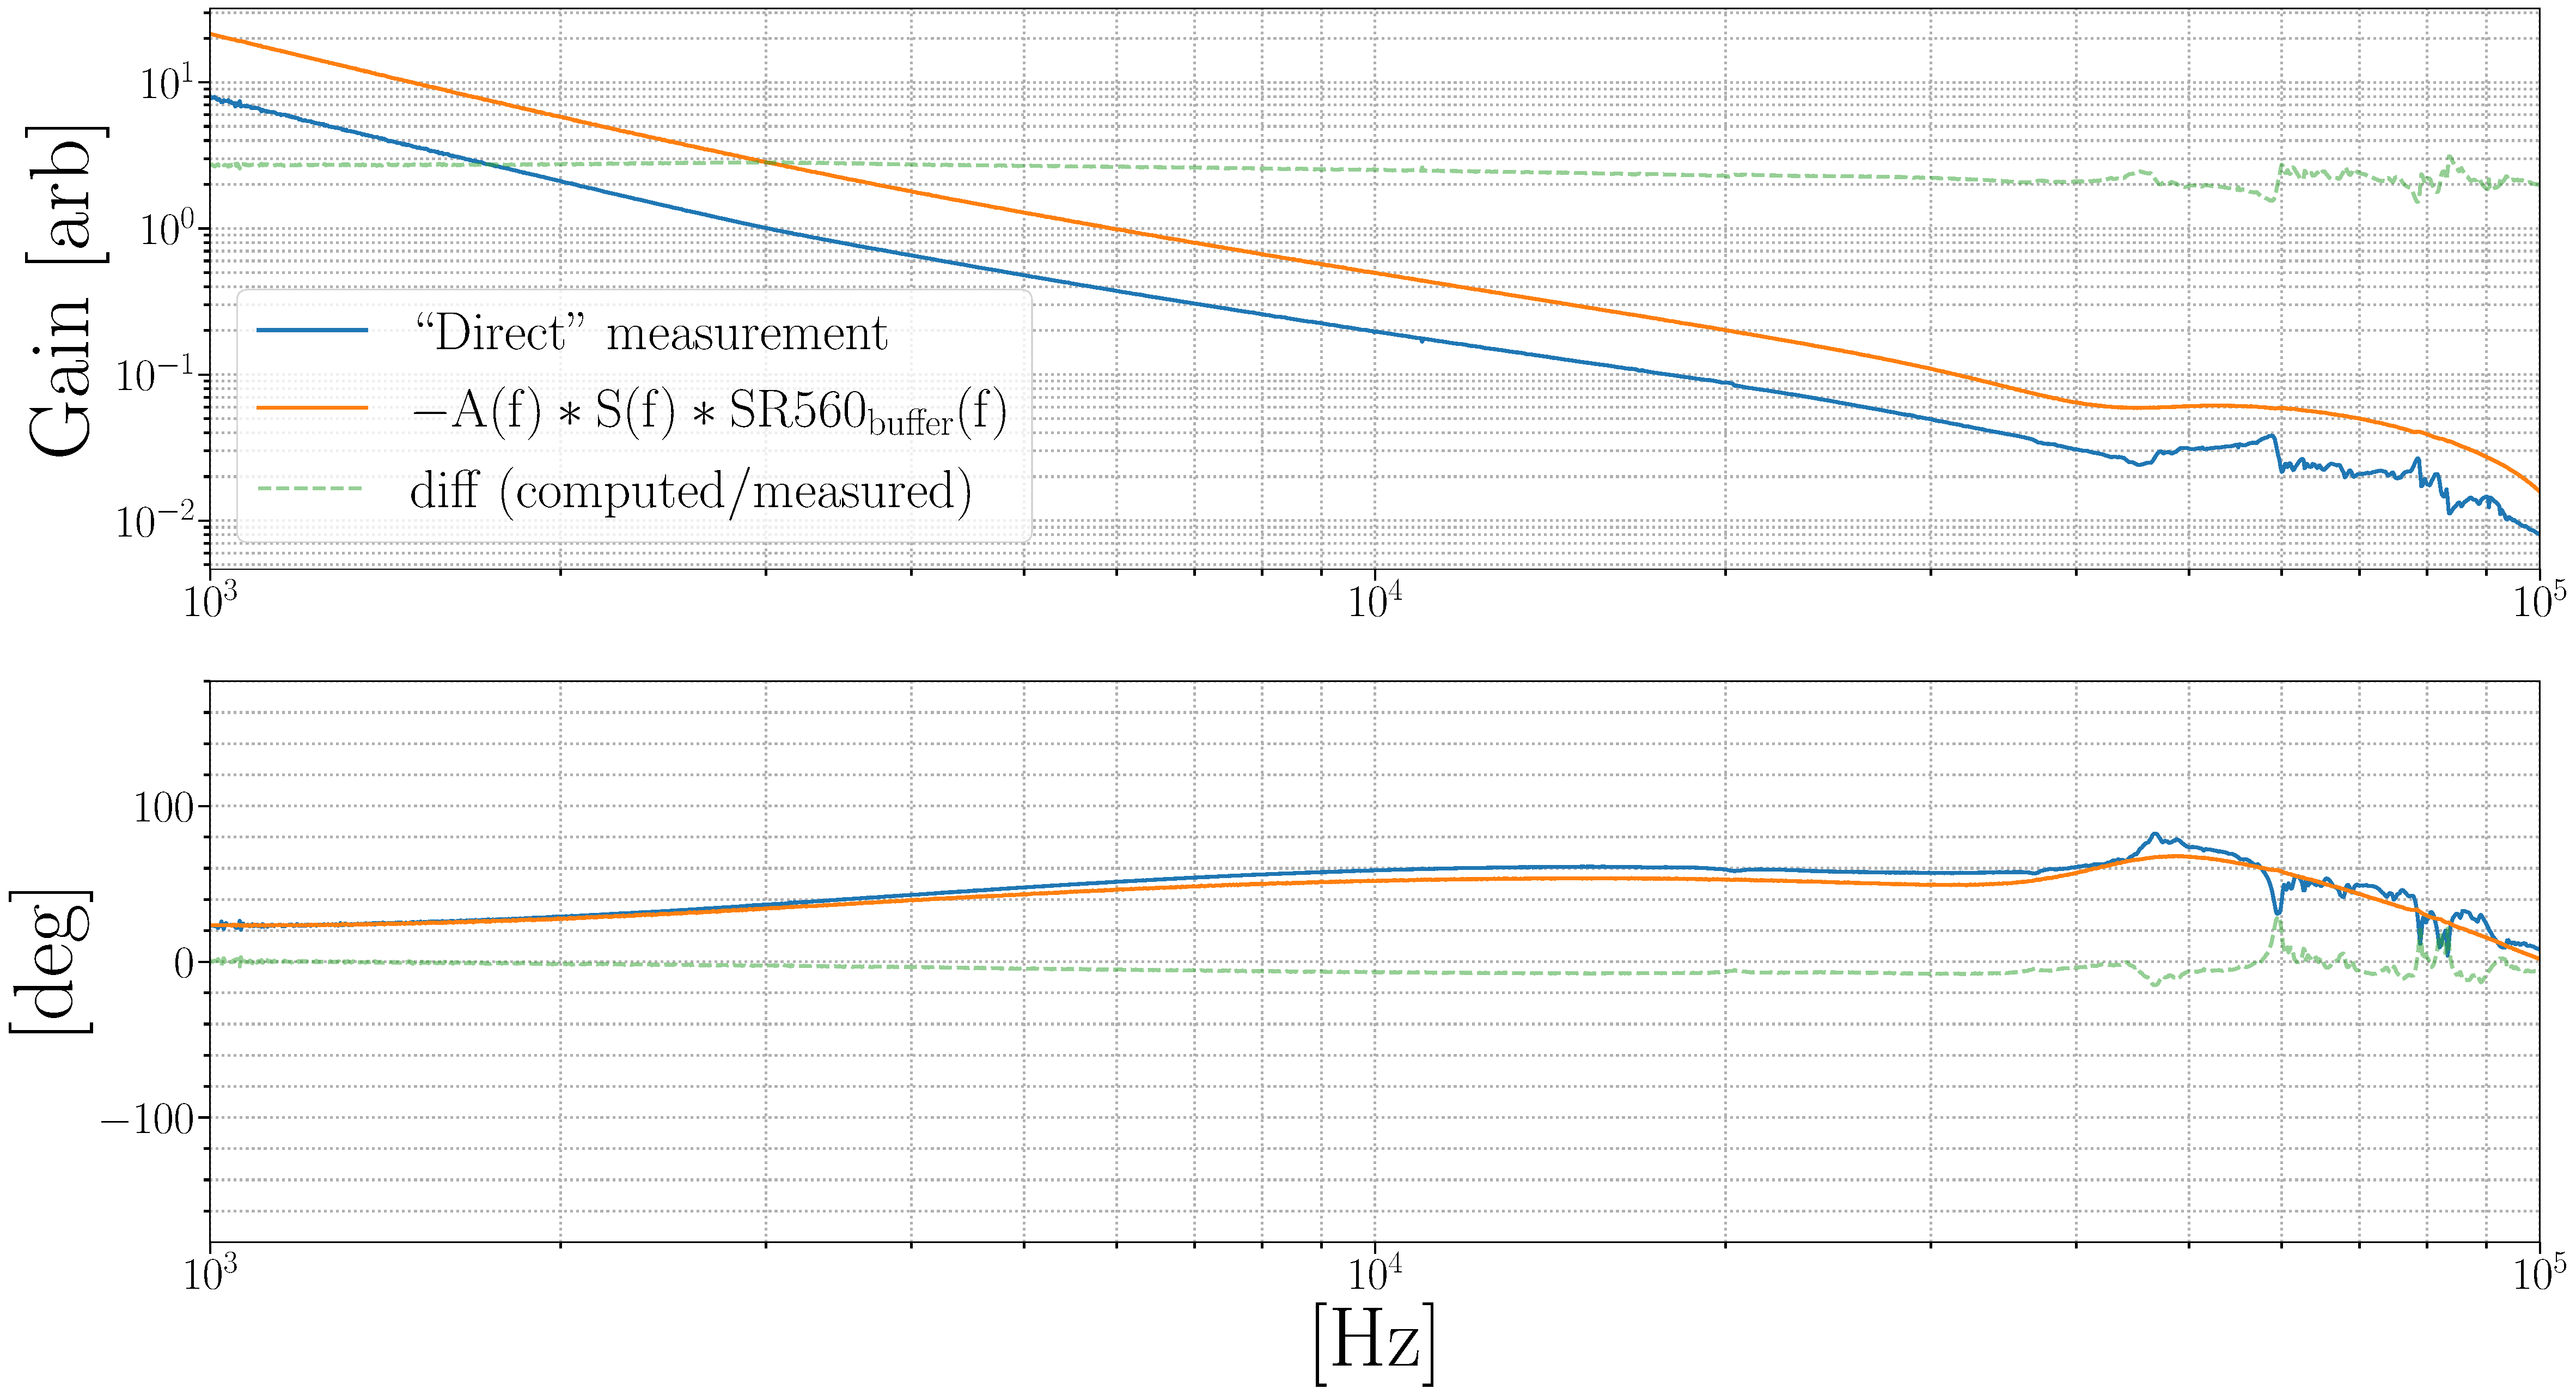
\includegraphics[width=\textwidth]{ALGAAS/olg_compare.pdf}
\end{center}
\caption{Comparison of the open loop gain measurement against the multiplied servo electronics measurements. The maximum gain difference is about a factor of 2.8 which is low passed to a difference of 2.0.}
\label{fig:OLGcompare}
\end{figure}

\subsection{Longitudinal Pockels Cell mirror mount assembly}
Maximizing a controlled and well defined electric field ($|E_z|$) within the coating while requiring a through beam to and through the HR coating lead us to a design very similar to that of a longitudinal pockels cell. The most common assembly used for this study is comprised of two electrodes with a 3mm central aperture which is chosen to be at least 5 times larger than the beam size at the plate locations; to avoid significant beam clipping while maximizing field strength ($\mathrm{E}_\mathrm{z}$) at the coating region of interest. There is also a required plate separation of at least 1/4" accounting for the thickness of the optical sample. Considering these constraints, modelling the system and computing the estimated field strength screened by the coating is the next step towards building the assembly.

\begin{figure}[H]
\begin{center}
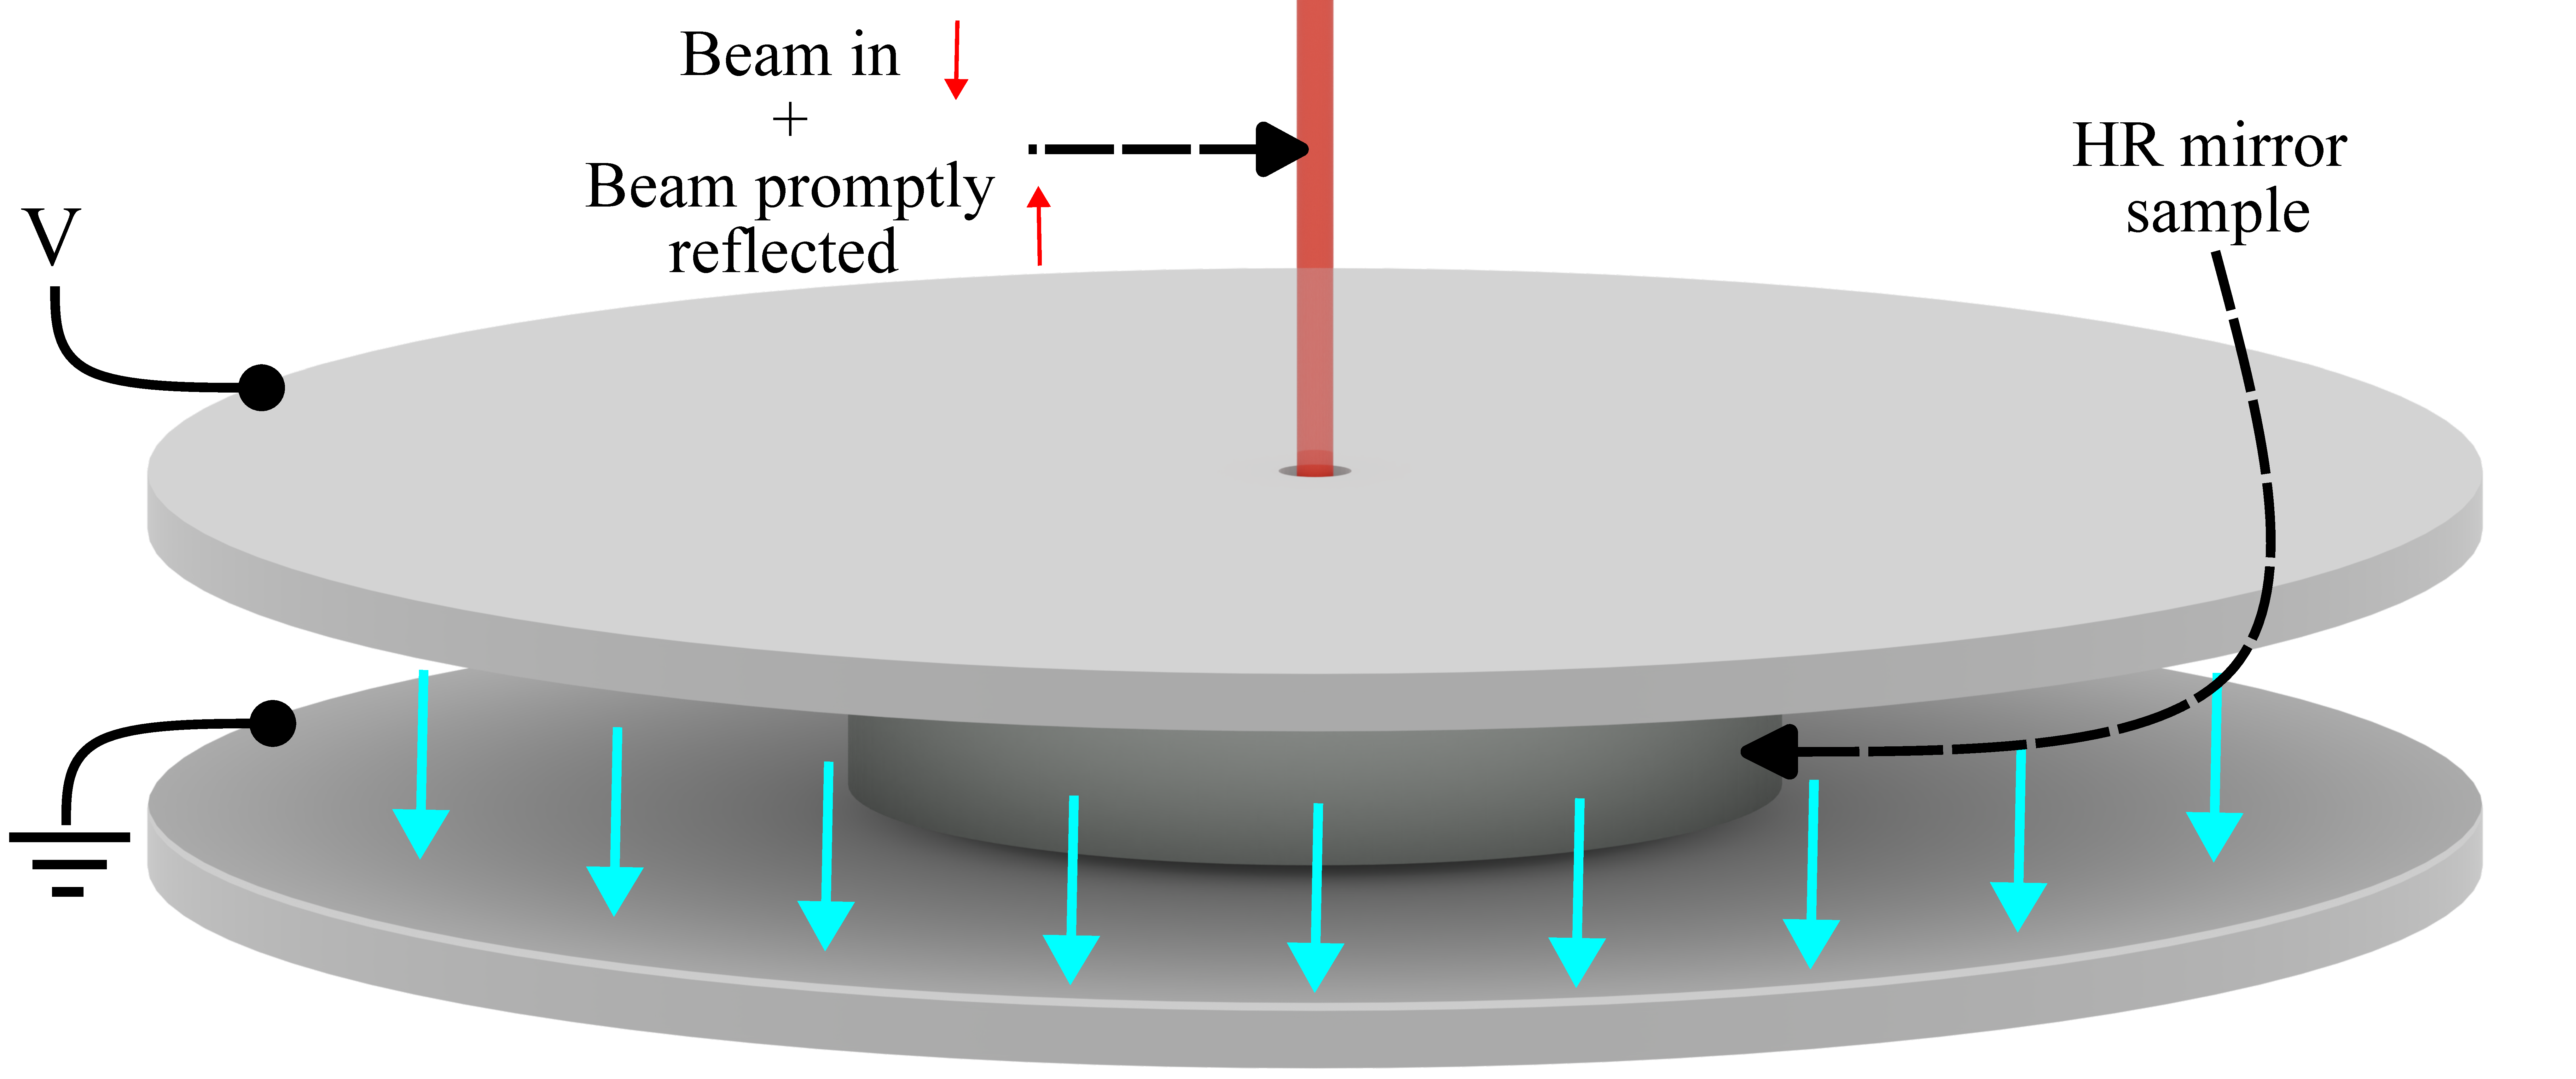
\includegraphics[width=\textwidth]{ALGAAS/longitudinal_pockels_cell_raw_isometric.pdf}
\end{center}
\caption{Concept image of the longitudinal Pockels cell assembly}
\label{fig:pckcellconcept}
\end{figure}

\subsubsection*{Modeling}
The field screened by the coating can be computed from Gauss' Law:
\begin{equation}
\nabla \cdot D = \rho_\mathrm{free}
\end{equation}

\noindent There is no free charge within the region of interest ($\rho_\mathrm{free}=0$), though the optic fused silica substrate with the AlGaAs coating imposes dielectric material between the plates. Boundary conditions are expressed in terms of the differential plate potential $V$, so it is natural to first solve the potential ($V(\mathrm{r, z})$) for all relevant system coordinate points.  

\begin{equation}\label{eq:cyllap}
\nabla^2 V = 0
\end{equation}

\paragraph*{Boundary Conditions}

\begin{figure}[H]
  \centering
  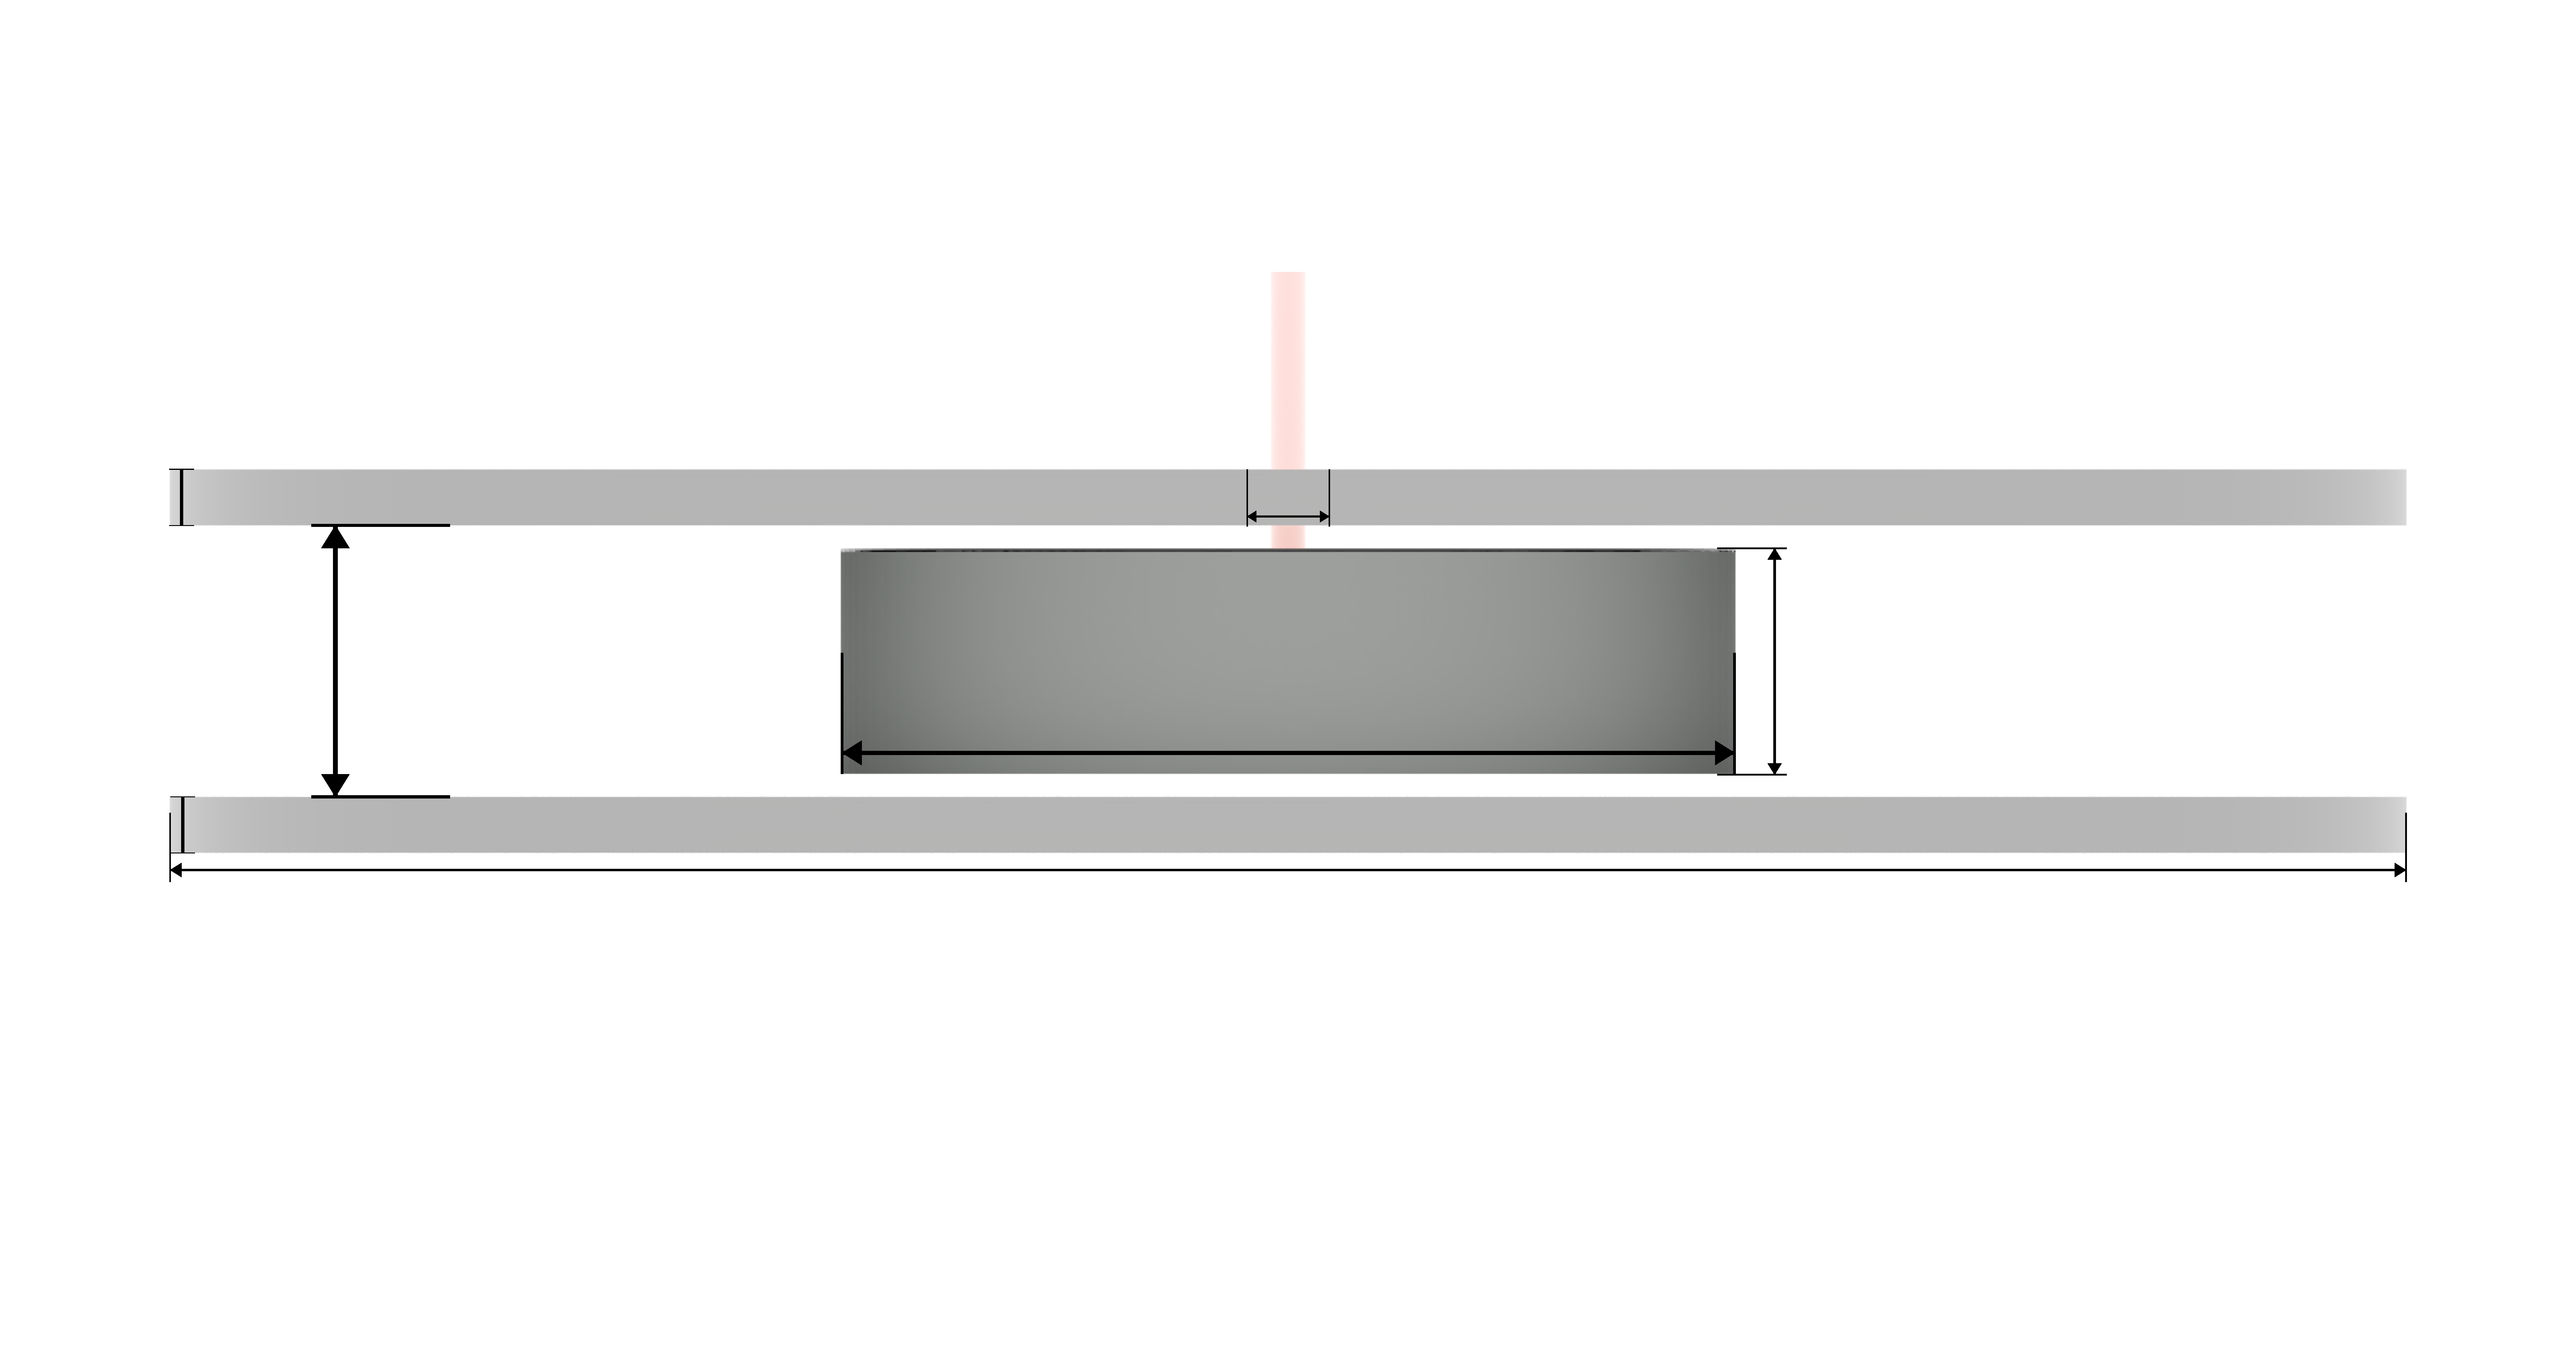
\includegraphics[width=\textwidth]{ALGAAS/longitudinal_pockels_cell_bc.pdf}
\caption{Side view of the longitudinal pockels cell mount. The figure is annotated with relevant parameters to build the numerical model: the finite thicknesses of the electrode plates ($t_{el}$) , radius of the aperture at the center of the disk ($r_{ap}$), radius of the disk ($r_d$),thickness of the optic ($t_{opt}$),and radius of the optic substrate ($r_{opt}$)}
  %%Use relevant cross sectional figure to establish coordinates for $\gaas$/$\algaas$, as well as the fused silica substrate so the computation is transparent.} Cross sectional diagram indicating relevant axes and boundary conditions utilized in the numerical computation
  \label{fig:laplacecoords}
\end{figure}

\subparagraph*{Substrate:}
$ -t_{opt} \; \textless \; z \; \textless \;\mathrm{t}_{opt} $ and $\mathrm{r} \; \textless \;\mathrm{r}_{opt}$
\subparagraph*{Coating}
$\mathrm{t}_{opt} \; \textless \; z \; \textless \;\mathrm{t}_{opt} +\mathrm{t}_{coat} $ and $\mathrm{r} \; \textless \;\mathrm{r}_{opt} $

\subparagraph*{Driven Electrode (V):}
$\mathrm{t}_{cap} \; \textless \; z \; \textless \;\mathrm{t}_{cap} + 2t_{el} $ and $\mathrm{r}_{ap} \; \textless \;\mathrm{r} \; \textless \;\mathrm{r}_{d} $

\subparagraph*{Grounded Electrode (GND):}
$ -t_{cap} -2t_{el} \; \textless \; z \; \textless \; -t_{cap} $ and $\mathrm{r}_{ap} \; \textless \;\mathrm{r} \; \textless \;\mathrm{r}_{d} $

\subparagraph*{Simulation Area Edges:}
$ z \; = \;\mathrm{z}_\mathrm{max} $ or  $r \; = \;\mathrm{r}_{max}$ or  $r \; = \;\mathrm{r}_{max}$ 
\\

\noindent For assured simulation convergence, an exponential falloff was applied to the simulation boundaries other than the (free) $\mathrm{r} = 0$ edge:

\begin{equation}
    \mathrm{Simulation \; Area \; Edges} \rightarrow A_o e^{(r+z)/r_o}
\end{equation}

Where $A_o$ is a characteristic voltage, and $r_o$ is a chosen characteristic distance. Though with the region of interest being at the coating surface, these edges are far enough away that a change in these characteristic values would cause a negligible difference to the resulting E-field estimate.

\subsubsection*{Computing V(r,z)}

Inspired by the second-order elliptic equation, operators are modified to incorporate the aforementioned boundary conditions ~\cite{Press:2007}.

\iffalse

\[ 
\mathcal{L}_{cyl} = 
\begin{bmatrix} \,
O_{n} & O_{n} & O_{n} & O_{n} & O_{n} & \cdots & \cdots & \cdots & \cdots & \cdots & O_{n}\\
\mathcal{I}_{n} & \mathcal{K}_{n}^{*} & \mathcal{I}_{n} & O_{n} & O_{n} & O_{n} & O_{n} & O_{n} & O_{n} & O_{n} & \vdots\\
O_{n} & \mathcal{I}_{n} & \mathcal{K}_{n}^{*} & \mathcal{I}_{n} & O_{n} & O_{n} & O_{n} & O_{n} & O_{n} & O_{n} & \vdots\\
O_{n} & O_{n}  & \mathcal{I}_{n} & \mathcal{K}_{n}^{*} & \mathcal{I}_{n} & O_{n} & O_{n} & O_{n} & O_{n} & O_{n} & \vdots\\
\vdots & O_{n}  & O_{n}  & \ddots & \ddots & \ddots & O_{n} & O_{n} & O_{n} & O_{n}  & \vdots \\
\vdots & O_{n}  & O_{n}  & O_{n}  & \ddots & \ddots & \ddots & O_{n} & O_{n} & O_{n} & \vdots \\
\vdots & O_{n}  & O_{n}  & O_{n} & O_{n} & \ddots & \ddots & \ddots & O_{n} & O_{n}  & \vdots \\
\vdots & O_{n}  & O_{n}  & O_{n} & O_{n} & O_{n} & \mathcal{I}_{n} & \mathcal{K}_{n}^{*} & \mathcal{I}_{n} & O_{n}  & \vdots\\
\vdots & O_{n}  & O_{n}  & O_{n} & O_{n} & O_{n} & O_{n} & \mathcal{I}_{n} & \mathcal{K}_{n}^{*}  & \mathcal{I}_{n} & O_{n}\\
\vdots & O_{n} & O_{n} & O_{n} & O_{n} & O_{n} & O_{n} & O_{n} & \mathcal{I}_{n} & \mathcal{K}_{n}^{*} & \mathcal{I}_{n}\\
O_{n}      & \cdots & \cdots & \cdots & \cdots & \cdots & O_{n} & O_{n} & O_{n} & O_{n} & {O}_{n}
\end{bmatrix} 
\]

\[
    \mathcal{K}_n^{(1)} = 
\frac{1}{h}
\begin{bmatrix*}[c] \,
0 & 0 & 0 & 0& 0 & \cdots & \cdots & \cdots & \cdots & \cdots & 0 \\
\frac{1}{2} & 0 & \frac{1}{2} & 0 & 0 & 0 & 0 & 0 & 0 & 0 & \vdots \\
0 & \frac{1}{4} & 0 & \frac{1}{4} & 0 & 0 & 0 & 0 & 0 & 0 & \vdots \\
0 & 0 & \frac{1}{6} & 0 & \frac{1}{6} & 0 & 0 & 0 & 0 & 0 & \vdots \\
\vdots & 0  & 0  & \ddots & \ddots & \ddots & 0 & 0 & 0 & 0  & \vdots \\
\vdots & 0  & 0  & 0  & \ddots & \ddots & \ddots & 0 & 0 & 0 & \vdots \\
\vdots & 0  & 0  & 0 & 0 & \ddots & \ddots & \ddots & 0 & 0  & \vdots \\
\vdots & 0  & 0  & 0 & 0 & 0 & \ddots & 0 & \frac{1}{2^{(n-4)}} & 0  & \vdots\\
\vdots & 0  & 0  & 0 & 0 & 0 & 0 & \frac{1}{2^{(n-3)}} & 0  & \frac{1}{2^{(n-3)}} & 0\\
\vdots & 0 & 0 & 0 & 0 & 0 & 0 & 0 & \frac{1}{2^{(n-2)}} & 0 & \frac{1}{2^{(n-2)}}\\
0      & \cdots & \cdots & \cdots & \cdots & \cdots & 0 & 0 & 0 & 0 & 0 
\end{bmatrix*}
\]

\[
    \mathcal{K}_n^{(2)}  = 
\frac{1}{h^2}
\begin{bmatrix} \,
-6 & 4 & 0 & 0& 0 & \cdots & \cdots & \cdots & \cdots & \cdots & 0 \\
1 & -4 & 1 & 0 & 0 & 0 & 0 & 0 & 0 & 0 & \vdots \\
0 & 1 & -4 & 1 & 0 & 0 & 0 & 0 & 0 & 0 & \vdots \\
0 & 0 & \ddots & \ddots & \ddots & 0 & 0 & 0 & 0 & 0 & 0 \\
\vdots & 0  & 0  & \ddots & \ddots & \ddots & 0 & 0 & 0 & 0  & \vdots \\
\vdots & 0  & 0  & 0  & \ddots & \ddots & \ddots & 0 & 0 & 0 & \vdots \\
\vdots & 0  & 0  & 0 & 0 & \ddots & \ddots & \ddots & 0 & 0  & \vdots \\
\vdots & 0  & 0  & 0 & 0 & 0 & \ddots & -4 & 1 & 0  & \vdots\\
\vdots & 0  & 0  & 0 & 0 & 0 & 0 & 1 & -4  & 1 & 0\\
\vdots & 0 & 0 & 0 & 0 & 0 & 0 & 0 & 1 & -4 & 1\\
0      & \cdots & \cdots & \cdots & \cdots & \cdots & 0 & 0 & 0 & 0 & 0 
\end{bmatrix}
\]

\[
	\mathcal{K}_n^{*} = \mathcal{K}_n^{(1)} + \mathcal{K}_n^{(2)} 
\]

\[
    \mathcal{I}_n = \frac{1}{h^2} \bigg( \mathrm{eye}(n) - \big( \mathrm{zeros}(n)[n,n] + 1 \big) \bigg)
\]

Where $\mathrm{eye}(\mathrm{n})$ and $\mathrm{zeros}({n})$ represent (nxn) identity and zero matrices respectively.

\[ 
	O_{n} = \mathrm{zeros}(n)
\]	
\fi

\iffalse
\begin{equation}
    V_{n + 1} = (\mathcal{I}_{N^2}  + \mathcal{L}_{cyl}) V_{n}
\end{equation}

Where the above matrix is a tri-diagonal block sparse matrix with square embedded diagonal identity ($\mathcal{I}_n$) matrices with n non-zero diagonal elements, and sparse tridiagonal kernel ($\mathcal{K}_n$) matrices. $O_n$ presents zero matrices with $n\times n$ sharing the dimensions of $\mathcal{K}_n$ and $\mathcal{I}_n$. \footnote{Not completely clear to the author at first, the motivation behind the structural choice of sparse block diagonals is a symptom of continuously vectorizing the computation. Some standard computing libraries may be proactive about this vectorization and apply it when recognized in for-loops. Even so, the explicit structuring of the boundary conditions listed here is intended to inform of the reasoning behind the modified numerical recipe to establish a compartmentalization between the scientific motivation alongside computing tools and methods.}
\fi


\begin{figure}[H]
  \centering
  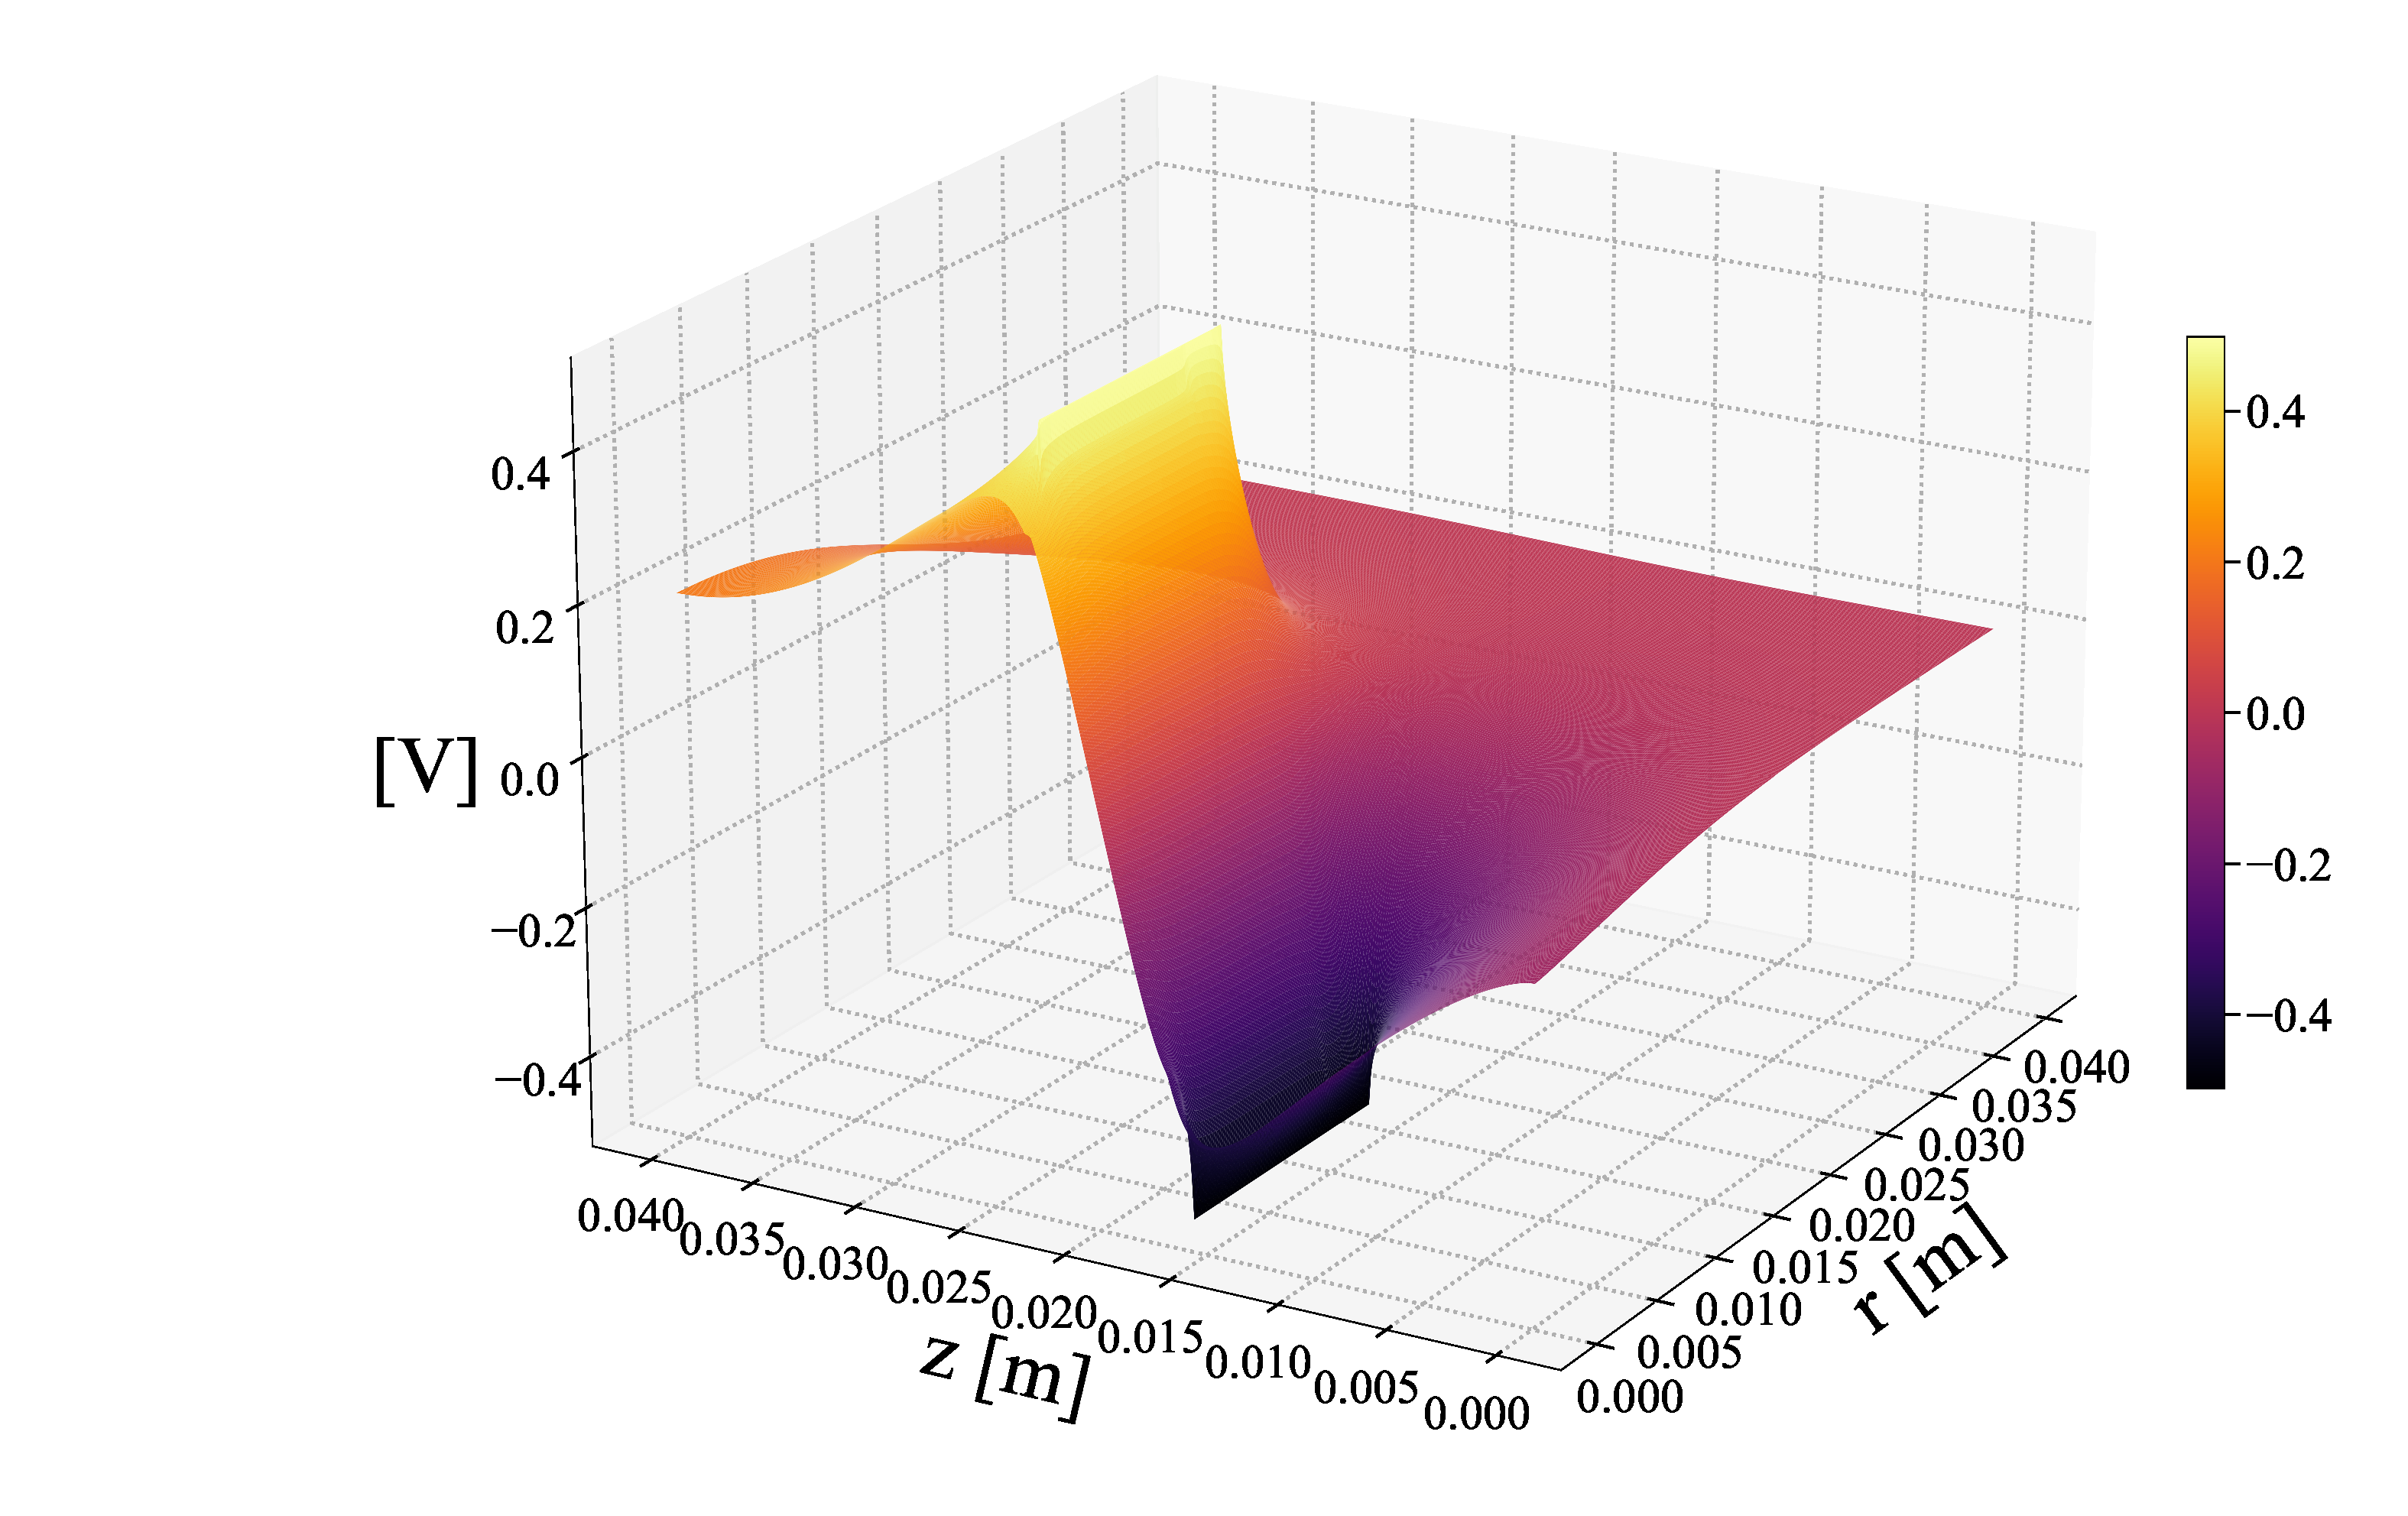
\includegraphics[width=.875\textwidth]{ALGAAS/assembly4_sim.pdf}
  \caption{Numerically computed potential map estimate ($V(z,r)$ in cylindrical coordinates). The potential difference between the two plates ($\Delta V$) is 1 [V] with a plate holding positive potential .5 [V] and a negative plate holding -.5 [V] to impose symmetry with the visualization. Although these held plate potentials differ from the 1 [V] and 0 [V] imposed in the experiment, the computation required to inform the field strength at the region of interest demonstrates a negligible difference between these two configurations.} 
  \label{fig:poissoncalcoutput}
\end{figure}


\subsubsection*{Computing $|\mathrm{E}_z|$(r,z)}

The computed $|\mathrm{E}_z|$ is screened by the coating at $r = 0$ for $V = 1$ and is estimated to be 13.3 $[\mathrm{V}/\mathrm{m}]$ and will be included in the calibration as a pockels cell conversion efficiency of 13.3 $[(\mathrm{V} / \mathrm{m}) / \mathrm{V}]$  

\begin{figure}[H]
    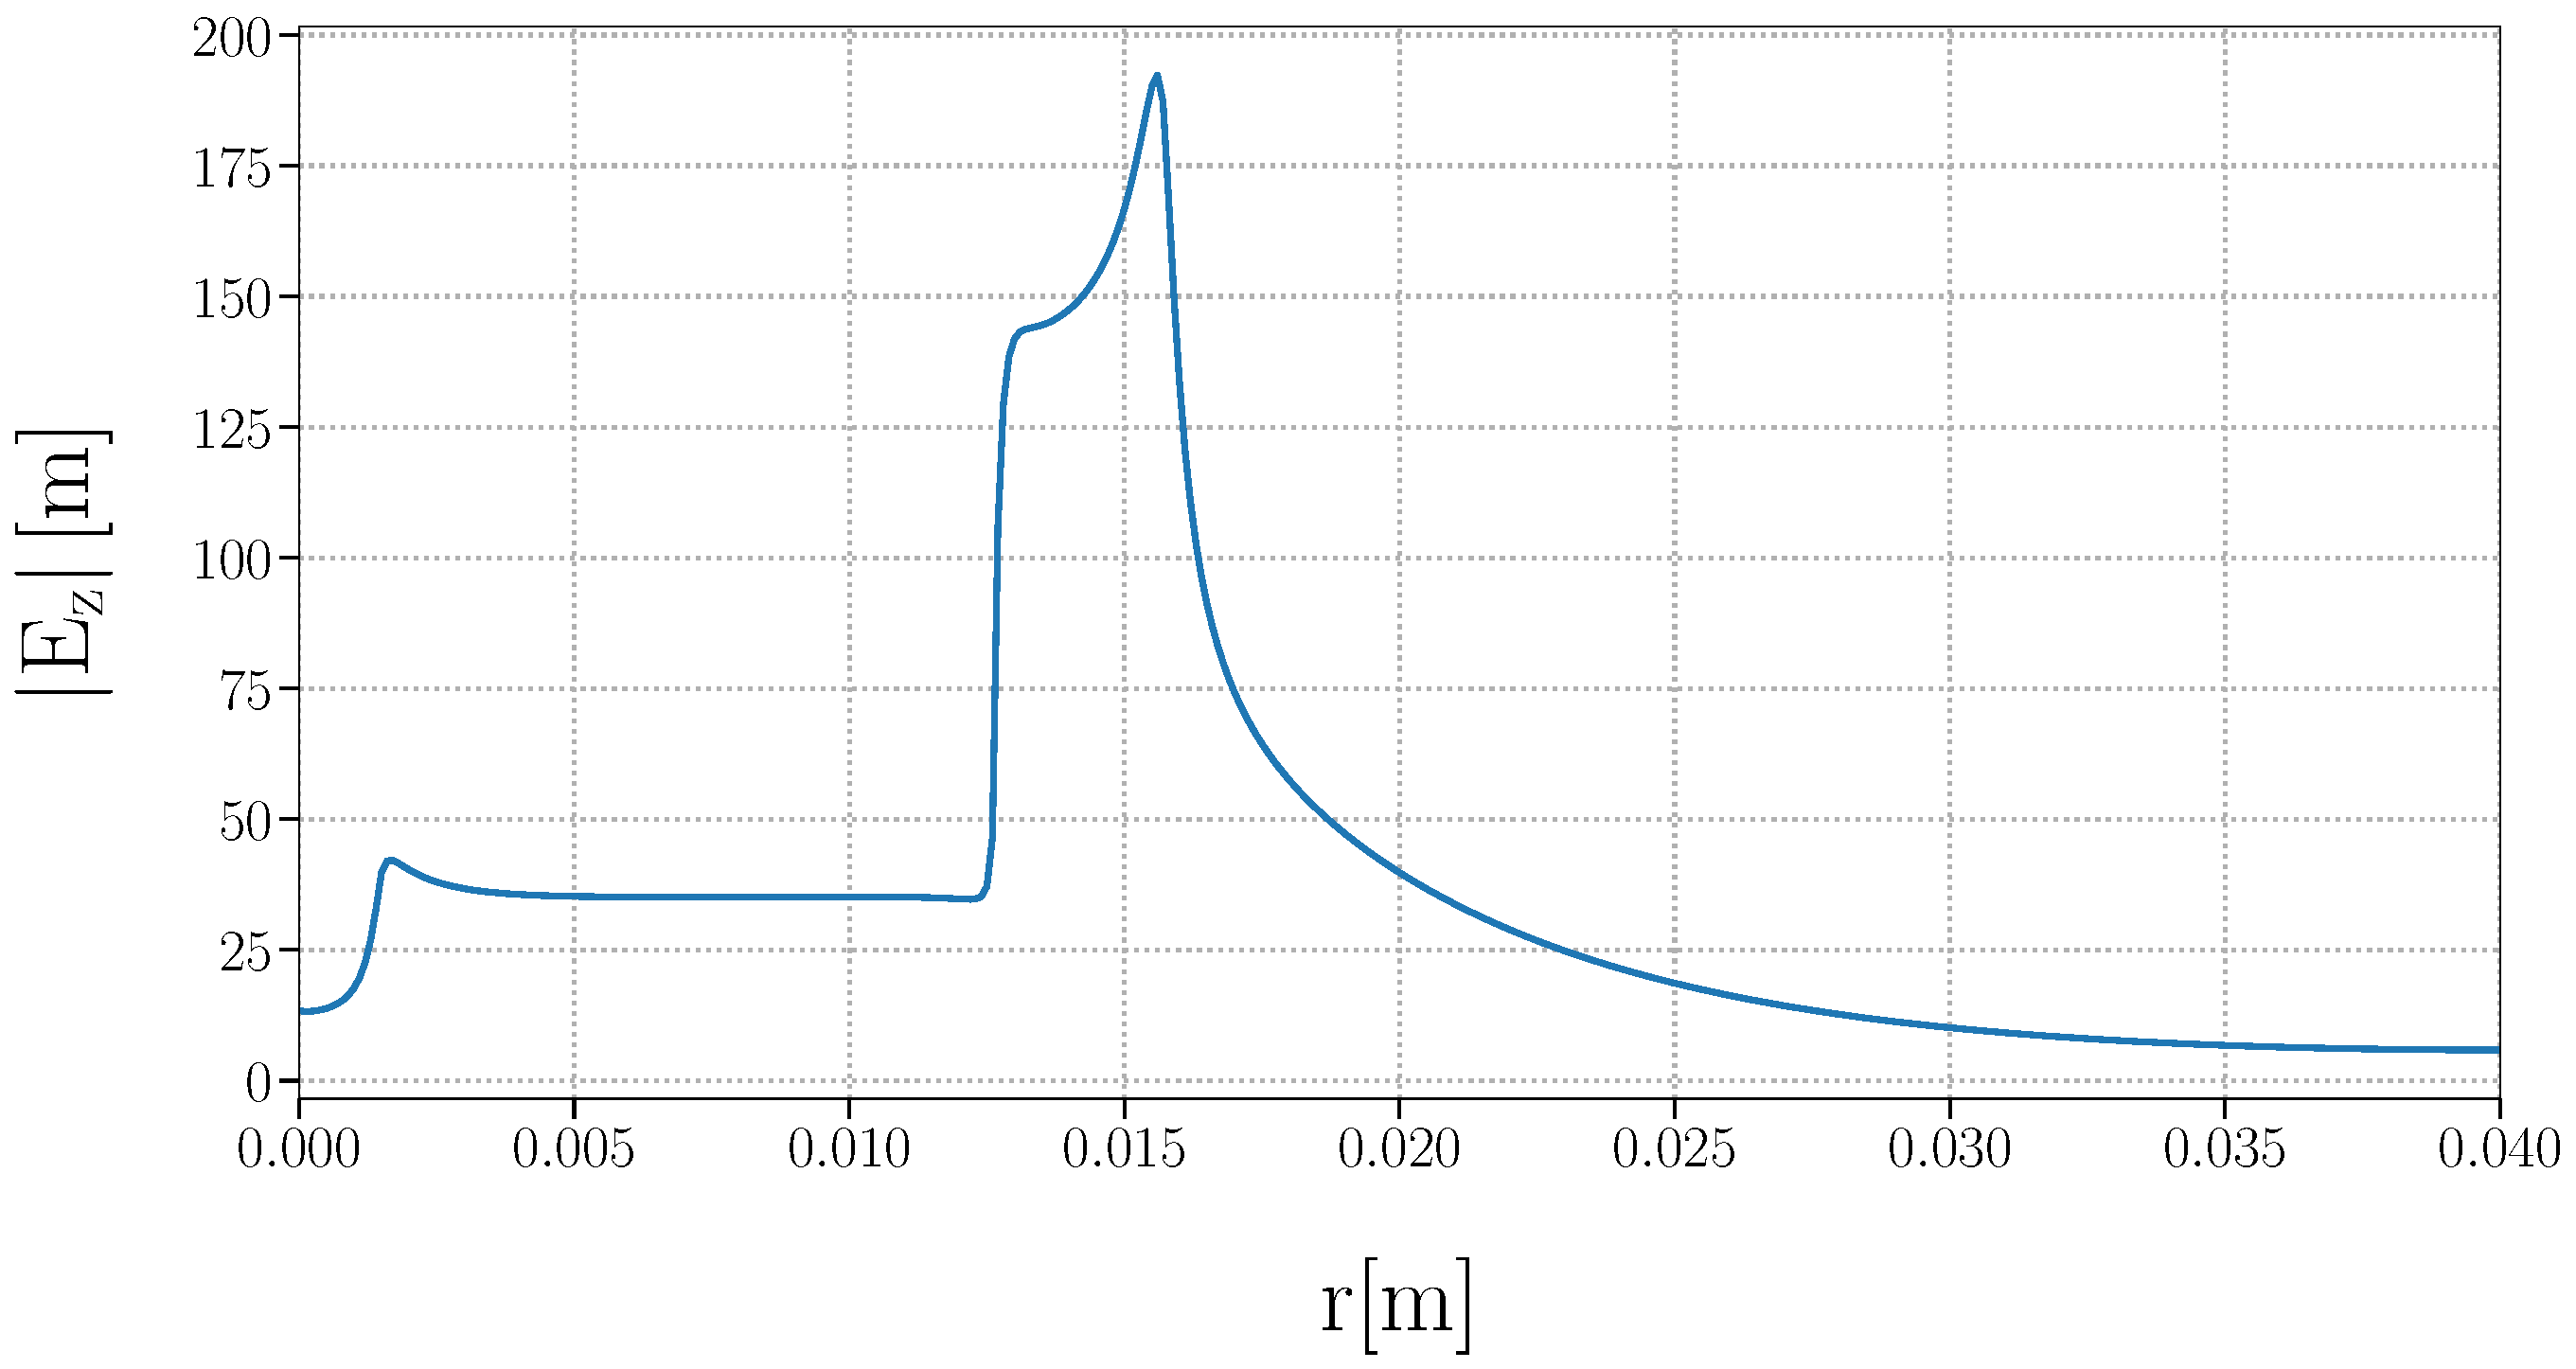
\includegraphics[width=\textwidth]{ALGAAS/fieldxsec_sim.pdf}
    \caption{Plot of the $| \mathrm{E}_\mathrm{z} |$ field cross section sampled about the optic HR coating surface.}
\label{fig:Ez}
\end{figure}

\iffalse
\subsection{Servo Overview}
\begin{figure}[!ht]
	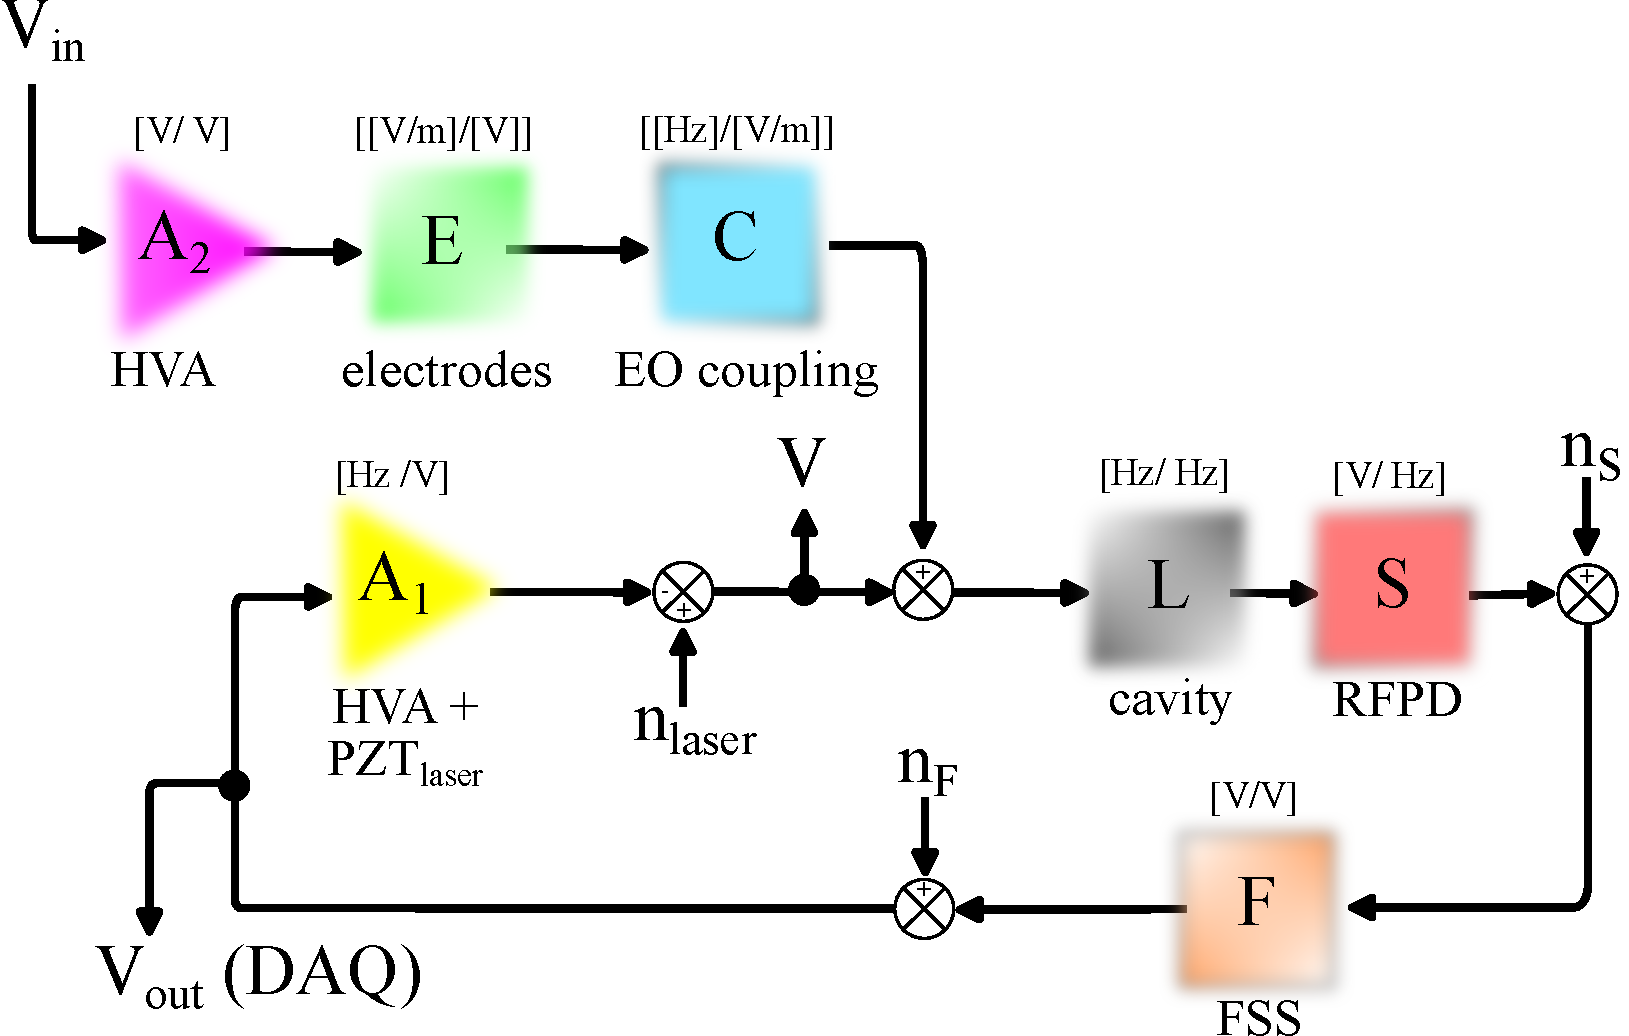
\includegraphics[width=\textwidth]{figs/ALGAAS/pock_control_diagram.pdf}
	\caption{A controls diagram of the designed servo.}
	\label{fig:pock_control_servo}
\end{figure}

\subsection{Calibration}



The  Electric field coupling can be expressed as a measured voltage:
$$\mathrm{V} = \frac{1}{1 + \mathrm{G}} \cdot \mathrm{n}_\mathrm{laser} - \frac{\mathrm{G}}{1 + \mathrm{G}} \cdot \mathrm{C}  \cdot \mathrm{E} \cdot \mathrm{A}_{2} \cdot \mathrm{V}_\mathrm{in} - \frac{\mathrm{F} \cdot \mathrm{A}_1}{1 + \mathrm{G}} \cdot \mathrm{n}_\mathrm{S} - \frac{A_1}{1 + \mathrm{G}} \cdot \mathrm{n}_\mathrm{F}$$
With G representing the open loop gain ($\mathrm{G} = \mathrm{A}_1 \cdot \mathrm{F} \cdot \mathrm{S} \cdot \mathrm{L}$). The feedback signal can also be represented as:

	\begin{align*} \mathrm{V}_\mathrm{out} & = \mathrm{F} \cdot \mathrm{S} \cdot \mathrm{L} \cdot (\mathrm{V} + \mathrm{C} \cdot \mathrm{E} \cdot \mathrm{A}_{2} \cdot \mathrm{V}_\mathrm{in}) + \mathrm{F} \cdot \mathrm{n}_\mathrm{S} + \mathrm{n}_\mathrm{F} \\ & = \frac{\mathrm{F} \cdot \mathrm{S} \cdot \mathrm{L}}{ 1 + \mathrm{G}} \cdot \mathrm{C} \cdot \mathrm{E} \cdot \mathrm{A}_{2} \cdot \mathrm{V}_\mathrm{in} + \frac{\mathrm{F} \cdot \mathrm{S} \cdot \mathrm{L}}{ 1 + \mathrm{G}} \cdot \mathrm{n}_\mathrm{laser} + \frac{\mathrm{F} }{ 1 + \mathrm{G}}\cdot \mathrm{n}_\mathrm{S} +  \frac{1}{ 1 + \mathrm{G}} \cdot \mathrm{n}_\mathrm{F} \end{align*}
Therefore $\frac{\mathrm{V}_\mathrm{out}}{\mathrm{V}_\mathrm{in}}$ : 
$$ \frac{\mathrm{V}_\mathrm{out}}{\mathrm{V}_\mathrm{in}} = \frac{\mathrm{F} \cdot \mathrm{S} \cdot \mathrm{L}}{1 + \mathrm{G}} \cdot \mathrm{C} \cdot \mathrm{E} \cdot \mathrm{A}_{2}  + \frac{\mathrm{F} \cdot \mathrm{S} \cdot \mathrm{L}}{ 1 + \mathrm{G}} \cdot \frac{\mathrm{n}_\mathrm{laser}}{\mathrm{V}_\mathrm{in}}+ \frac{\mathrm{F} }{ 1 + \mathrm{G}} \cdot \frac{\mathrm{n}_\mathrm{S}}{\mathrm{V}_\mathrm{in}} +  \frac{1}{ 1 + \mathrm{G}} \cdot \frac{\mathrm{n}_\mathrm{F}}{\mathrm{V}_\mathrm{in}}$$
\swb{The above is not a transfer function. Either express $V_{in}$ as function of all inputs, or, if you want a true transfer function, set all  inputs except $V_{in}$ to 0, so only keet the first term in the above equation.}
If the induced excitation is larger than the noise  we approximate the last equation:

$$ \frac{\mathrm{V}_\mathrm{out}}{\mathrm{V_{in}}} \approx \frac{\mathrm{F} \cdot \mathrm{S} \cdot \mathrm{L}}{1 + \mathrm{G}} \cdot \mathrm{C} \cdot \mathrm{E} \cdot \mathrm{A}_{2} = \frac{\mathrm{G}}{1 + \mathrm{G}} \cdot \mathrm{C} \cdot \mathrm{E} \cdot \frac{\mathrm{A}_{2}}{\mathrm{A}_{1}} $$
 \swb{The second piece is not correct, singe G = A1*F*S*L.}

\subsubsection{OLG(f)}
\begin{figure}[H]
  \begin{center}
    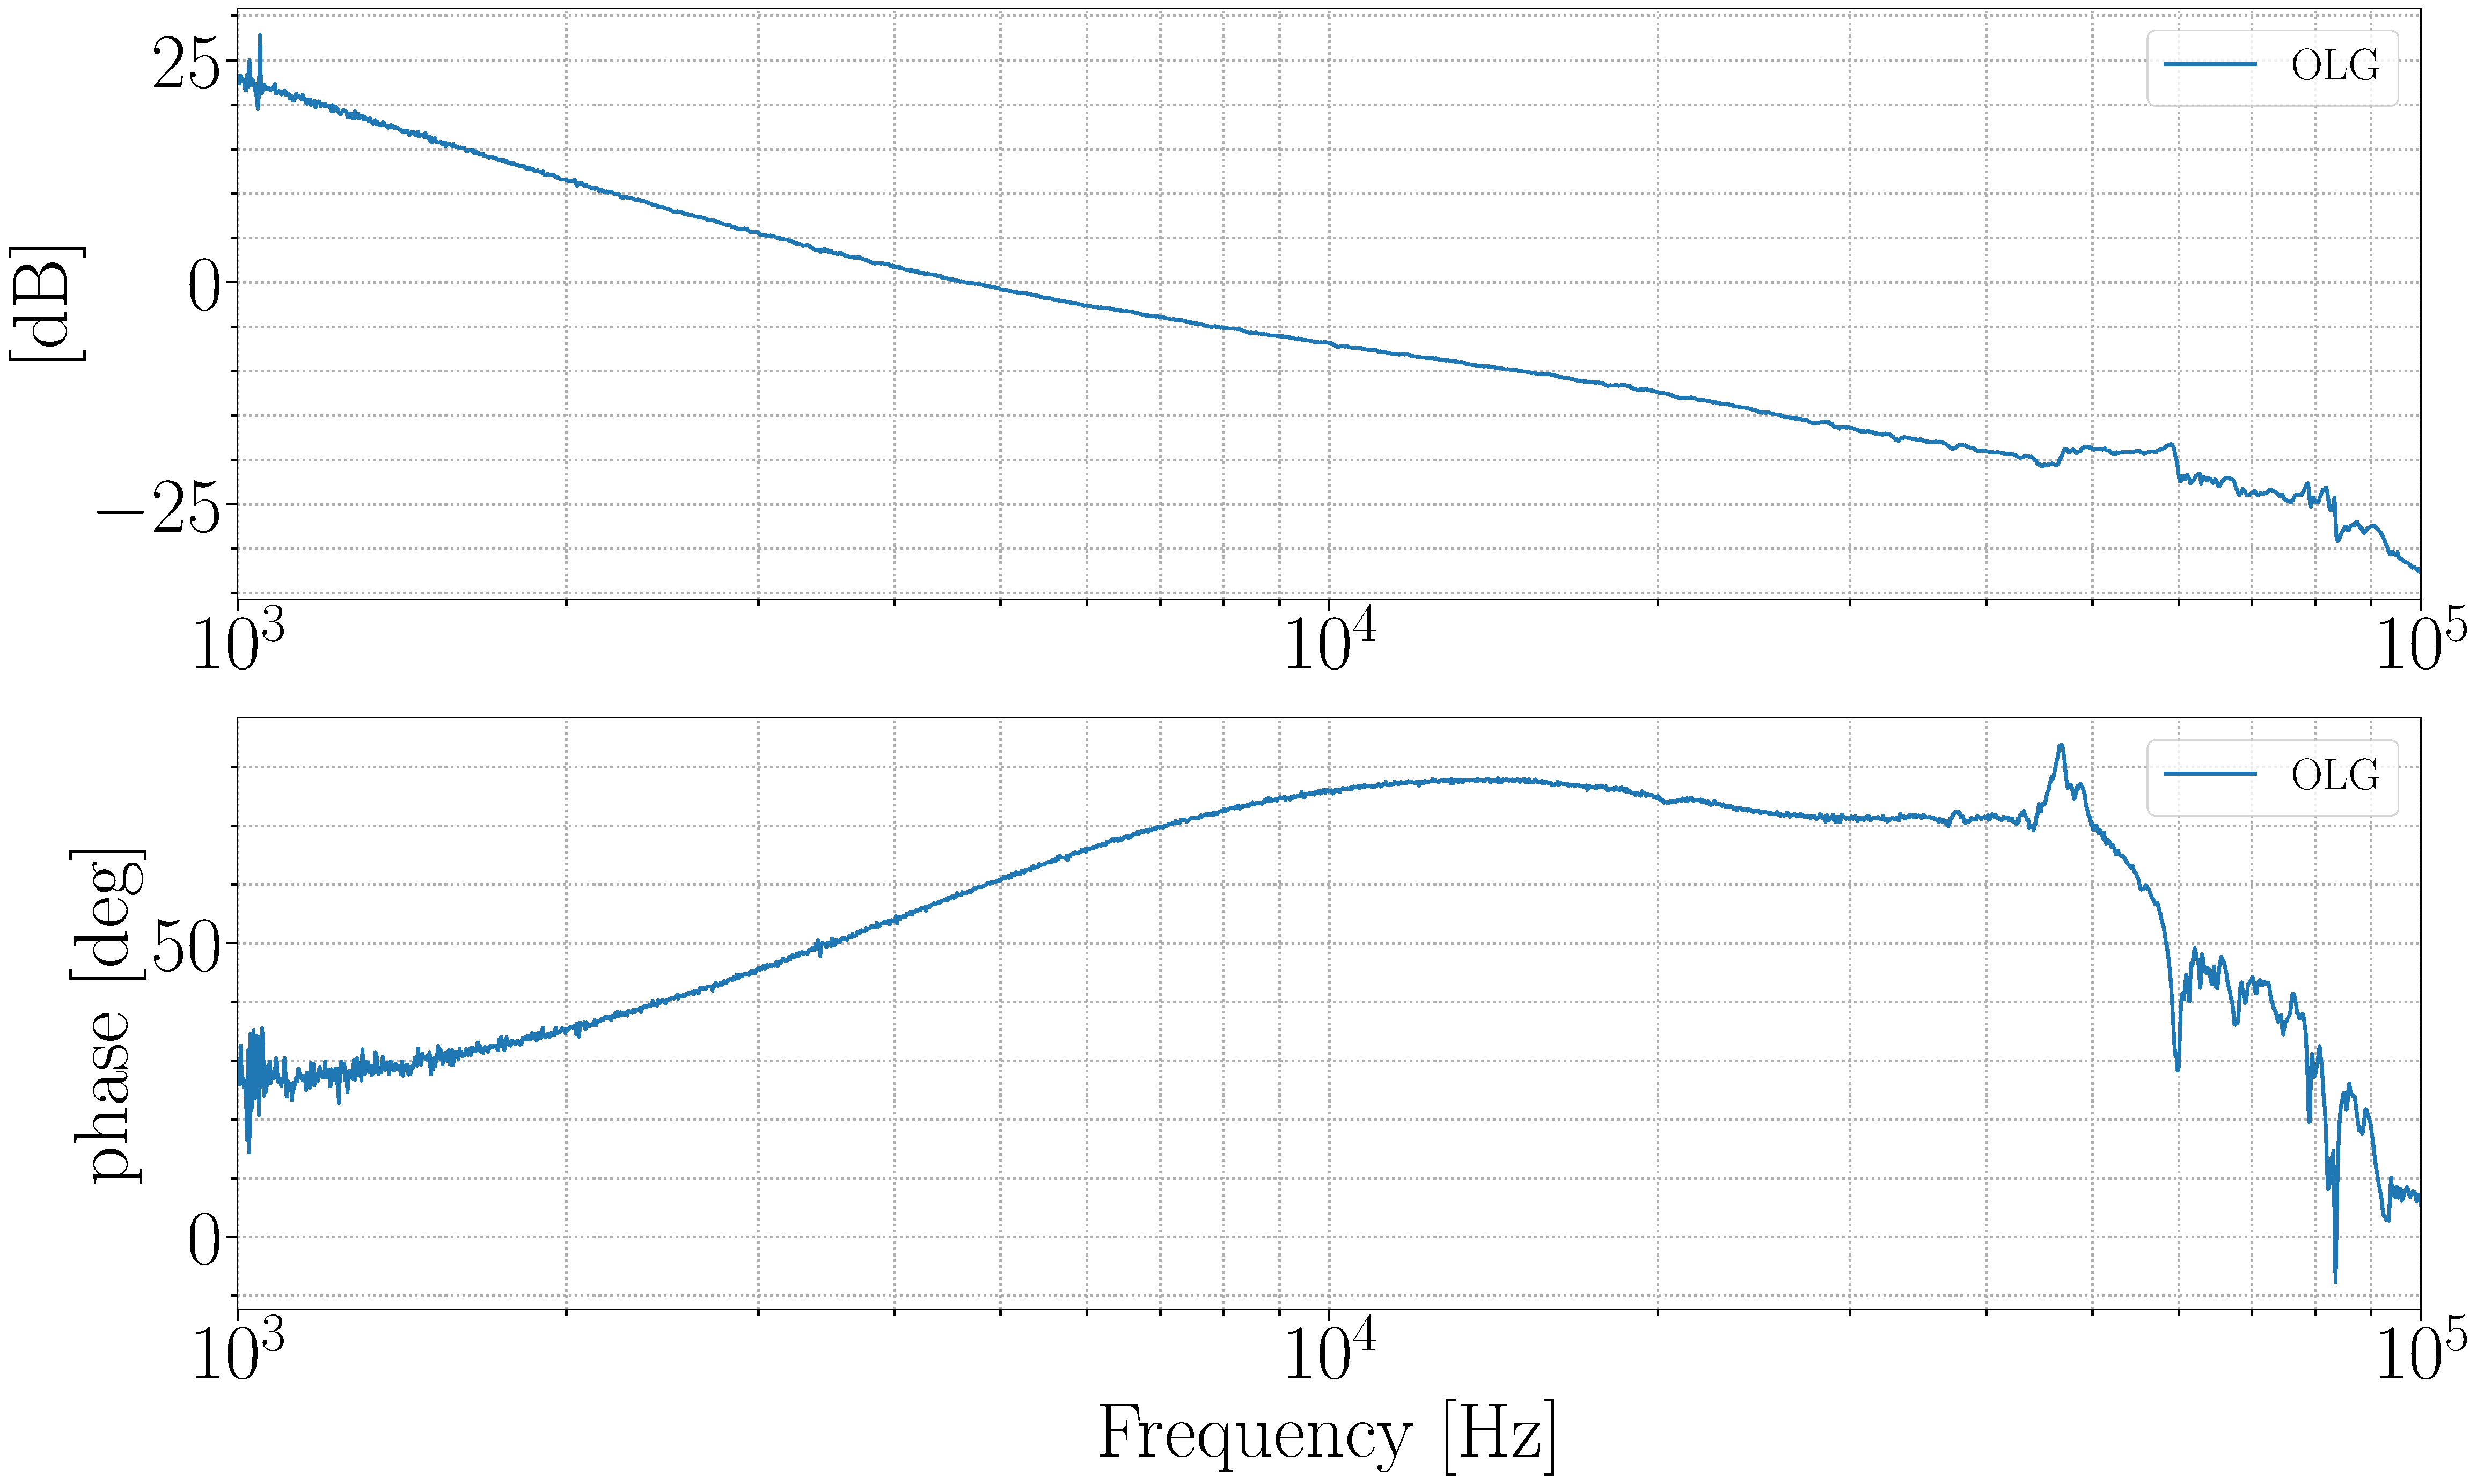
\includegraphics[width=\textwidth]{figs/ALGAAS/tfs/OLG.pdf}
    \caption{Measurement of the OLG taken as noted in \autoref{appendix:OLG_meas}}
  \end{center}
  \label{fig:OLGmeas}
\end{figure}

\swb{You need some context for this. What is this the OLG of?}

The calibration math for this measurement explicitly starts with what I
call \(\alpha(f)\) which is a vector of complex numbers that represents
the transfer function \(\mathrm{CH2}(f)/\mathrm{CH1}(f)\) where:

\[\mathrm{CH1}(f) = \mathrm{Source}(f)\] and
\[\mathrm{CH2}(f) = \frac{\mathrm{S}(f)* signal(f)}{1-\mathrm{OLG}(f)}\]

Where \[\mathrm{OLG}(f) = \mathrm{A}(f)* \mathrm{S}(f)\]

and \(signal(f)\) is the demodulated output from
\(\mathrm{RFPD}_\mathrm{refl}\) and \(\mathrm{S}(f)\) is the transfer
function of the frequency stabilization servo.

From here we solve for signal(f):

\[signal(f) = \mathrm{CH2}(f) * \mathrm{A}_{1}(f) * \mathrm{A}_2* \frac{(1-\mathrm{OLG}(f))}{\mathrm{OLG}(f)}\]

Where \(\mathrm{A}_{1}(f)\) informs the frequency dependent drive sent
to the laser PZT to keep the cavity locked and \(\mathrm{A}_2\) is the
laser frequency detuning factor {[}Hz/V{]} (can be estimated from
measuring PDH).

Currently \(signal(f)\) provides a frequency noise spectra which then
can be converted into a displacement spectra with the following
relation:

\[\frac{\Delta f}{f_\mathrm{laser}} = \frac{\Delta L}{L_\mathrm{cav}}\]

This allows us to imagine the frequency noise spectra as a length noise
spectra due to the drive on the electrodes:

\[signal(f) = \alpha(f)* \mathrm{Source}(f) * \mathrm{A}_{1}(f) * \mathrm{A}_2* \frac{(1-\mathrm{OLG}(f))}{\mathrm{OLG}(f)} * \frac{L_\mathrm{cav}}{f_\mathrm{laser}}\hspace{35pt} [m_\mathrm{pk}]\]

And for the measurement normalized by the drive voltage on the
electrodes:

\[\frac{signal(f)}{\mathrm{Source}(f) * \mathrm{G}(f)} = \frac{\alpha(f)}{\mathrm{G}(f)} * \mathrm{A}_{1}(f) * \mathrm{A}_2* \frac{(1-\mathrm{OLG}(f))}{\mathrm{OLG}(f)} * \frac{L_\mathrm{cav}}{f_\mathrm{laser}}\hspace{35pt} \bigg[\frac{m_\mathrm{pk}}{V_\mathrm{pk}}\bigg]\]
\#\# Noise or single frequency drive measurement : \(n(f)\) The
calibration math for this measurement is essentially equivalent to the
transfer function measurement above. The only difference is:

\[\mathrm{CH1}(f) = \frac{\mathrm{S}(f)* signal(f)}{1-\mathrm{OLG}(f)}\]

and

\[signal(f) = \mathrm{CH1}(f) * \mathrm{A}_{1}(f) * \mathrm{A}_2* \frac{(1-\mathrm{OLG}(f))}{\mathrm{OLG}(f)} * \frac{L_\mathrm{cav}}{f_\mathrm{laser}}\]

Where \(signal(f)\) in this measurement represents the free running
cavity displacement noise with the exception of a single frequency if it
is not a noise measurement.

If \(\mathrm{CH1}(f)\) is in \(\frac{V_\mathrm{rms}}{\sqrt{Hz}}\) then
signal(f) will be in \(\frac{m_\mathrm{rms}}{\sqrt{Hz}}\)

or

If \(\mathrm{CH1}(f)\) is in \(V_\mathrm{pk}\) then signal(f) will be in
\(m_\mathrm{pk}\) 
\fi

%\#\# Calibration code
%The error signal spectra probed at the FSS:
%\begin{equation}
%\mathrm{VFSSOUT}_\mathrm{rms}/\sqrt{Hz} \rightarrow m_\mathrm{rms}/\sqrt{\mathrm{Hz}}
%\end{equation}
%With the known frequency response of the servo electronics, we \autoref{sec:calibration} the measurement into differential length:
%\begin{equation}
%	\Delta \mathrm{L} = \mathrm{source}*\alpha(f) \mathrm{A}(f)*\frac{1+\mathrm{OLG}(f)}{\mathrm{OLG}(f)}*\frac{\mathrm{L_{cav}}}{f_\mathrm{laser}} \quad \big[ m_\mathrm{pk} / \sqrt{Hz} \big]
%\end{equation}

\subsection{Assembly Mount Tests/Development}
The following section briefly discusses the nature of early measurements performed with various longitudinal pockel cell mount assemblies. A significant barrier to low differential length noise sensitivity for this experiment was the lack of low-noise optical mounts in accessible non-conductive materials. Most commercial optical mounts are constructed with conductive materials which is problematic when seeking to isolate the coating from non-normal field gradients within the coating volume of interest.  For this reason, efforts were focused on developing a suitable mounting solution that would provide adequate isolation from any uncontrolled field magnitudes while driving a field normally incident on the surface with enough strength and uniformity across the beam area to extract a measurement of the differential length change from the Pockels effect. 3D printing for this project was inititally used as a means to prototype optical mount designs but public health concerns at the time made testing with alternative materials aside from PLA and PETG difficult. There were multiple 3D prints tested within the optical schema depicted in \autoref{fig:simpschema}. 

\subsubsection{Assembly 0 and 1}

\paragraph*{Model params}
\begin{center}
\begin{tabular}{ |c|c|c|c|c|c| } 
\hline
$\mathrm{r}_{ap}$ [m] &  $\mathrm{t}_{cap}$ [m] & $\mathrm{r}_{el}$ [m] & $\mathrm{t}_{el}$ [m] & $\mathrm{r}_{opt}$ [m] & $\mathrm{t}_{opt}$ [m] \\
\hline
1.5e-3 & 4.5e-3 & 38.1e-3 & 1.5e-3 & 12.7e-3 & 6.35e-3 \\ 
\hline
\end{tabular}
\end{center}

\paragraph*{Electrodes}
\begin{figure}[H]
  \centering
  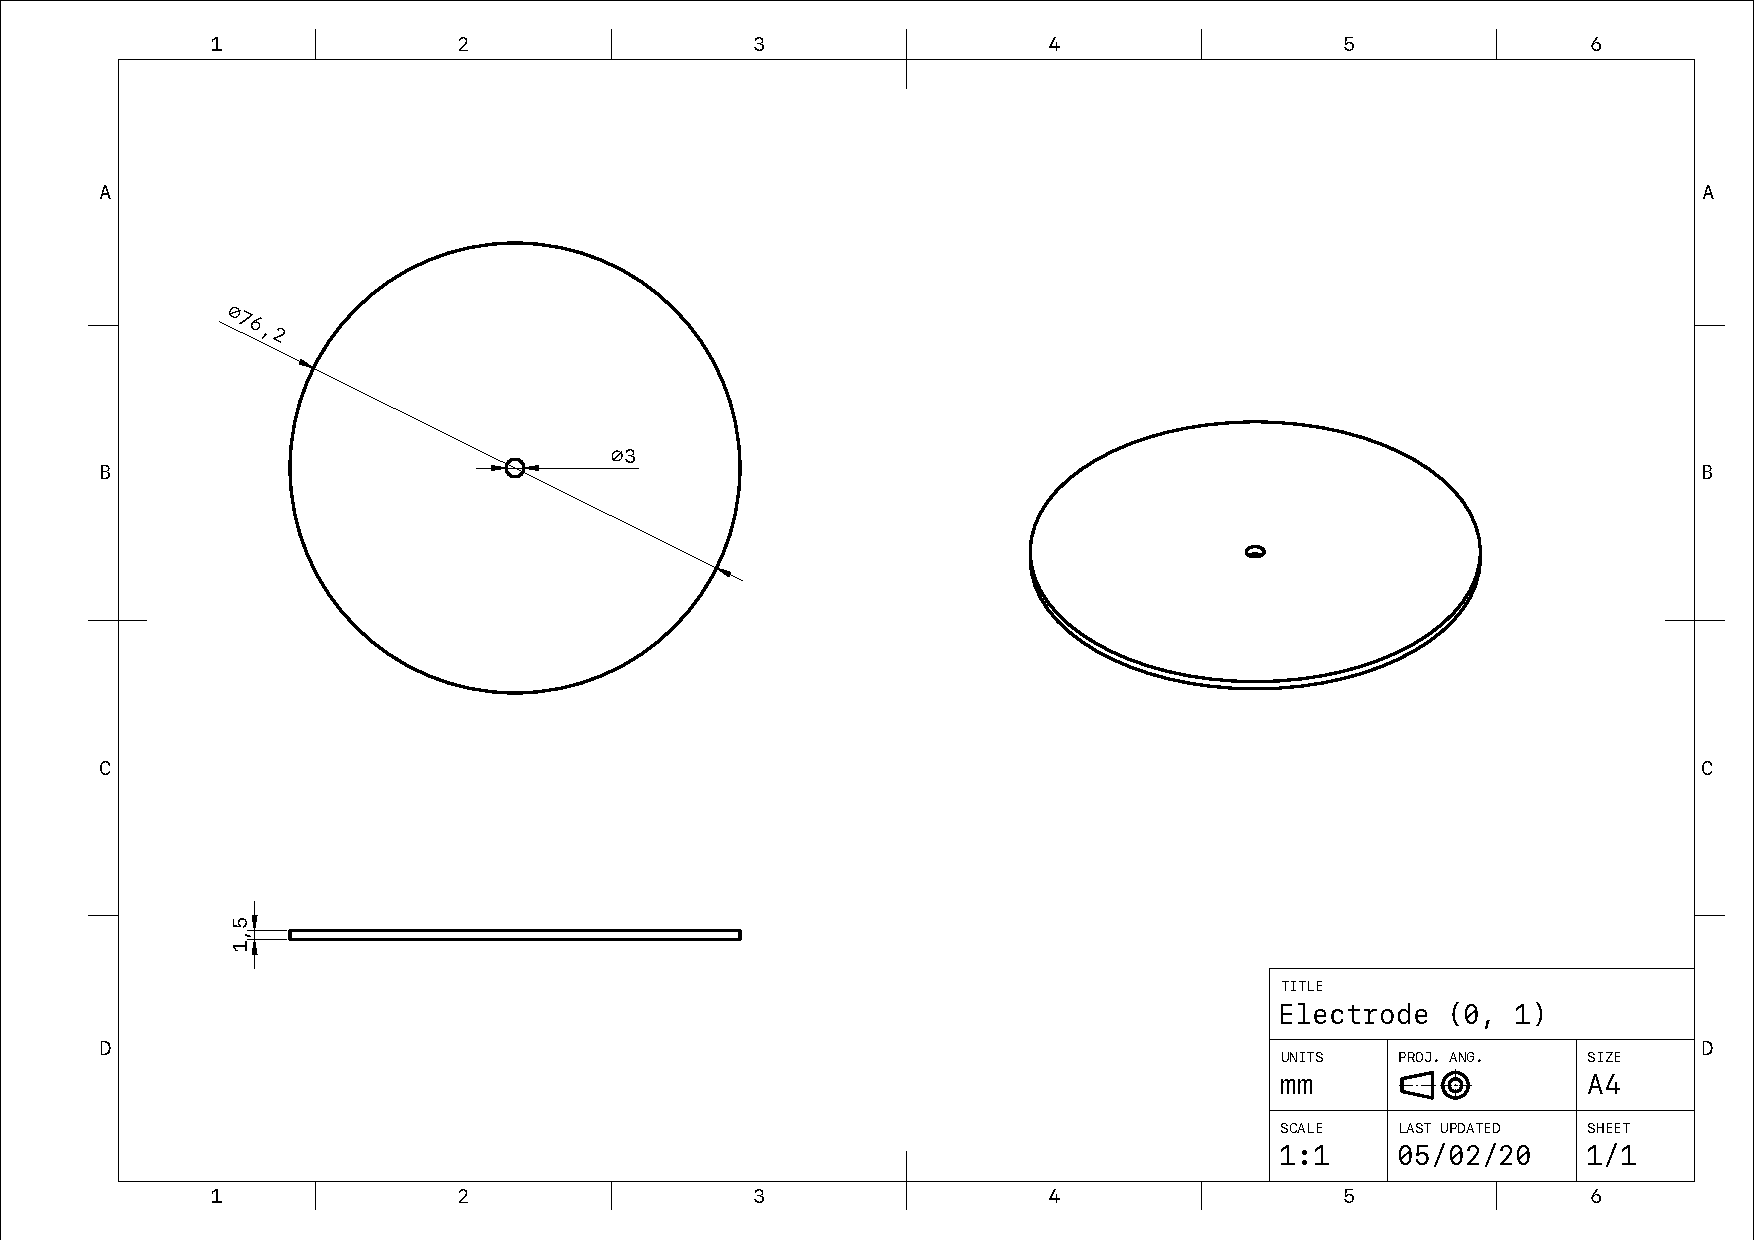
\includegraphics[width=\textwidth]{figs/ALGAAS/assemblies/assembly0/Electrode_0_1.pdf}
  \caption{Technical drawing of the 3" disk electrode plates made of aluminum.}
\end{figure}


\paragraph*{Mount 0}

\begin{figure}[!ht]
	\begin{subcaptiongroup}
		\centering
		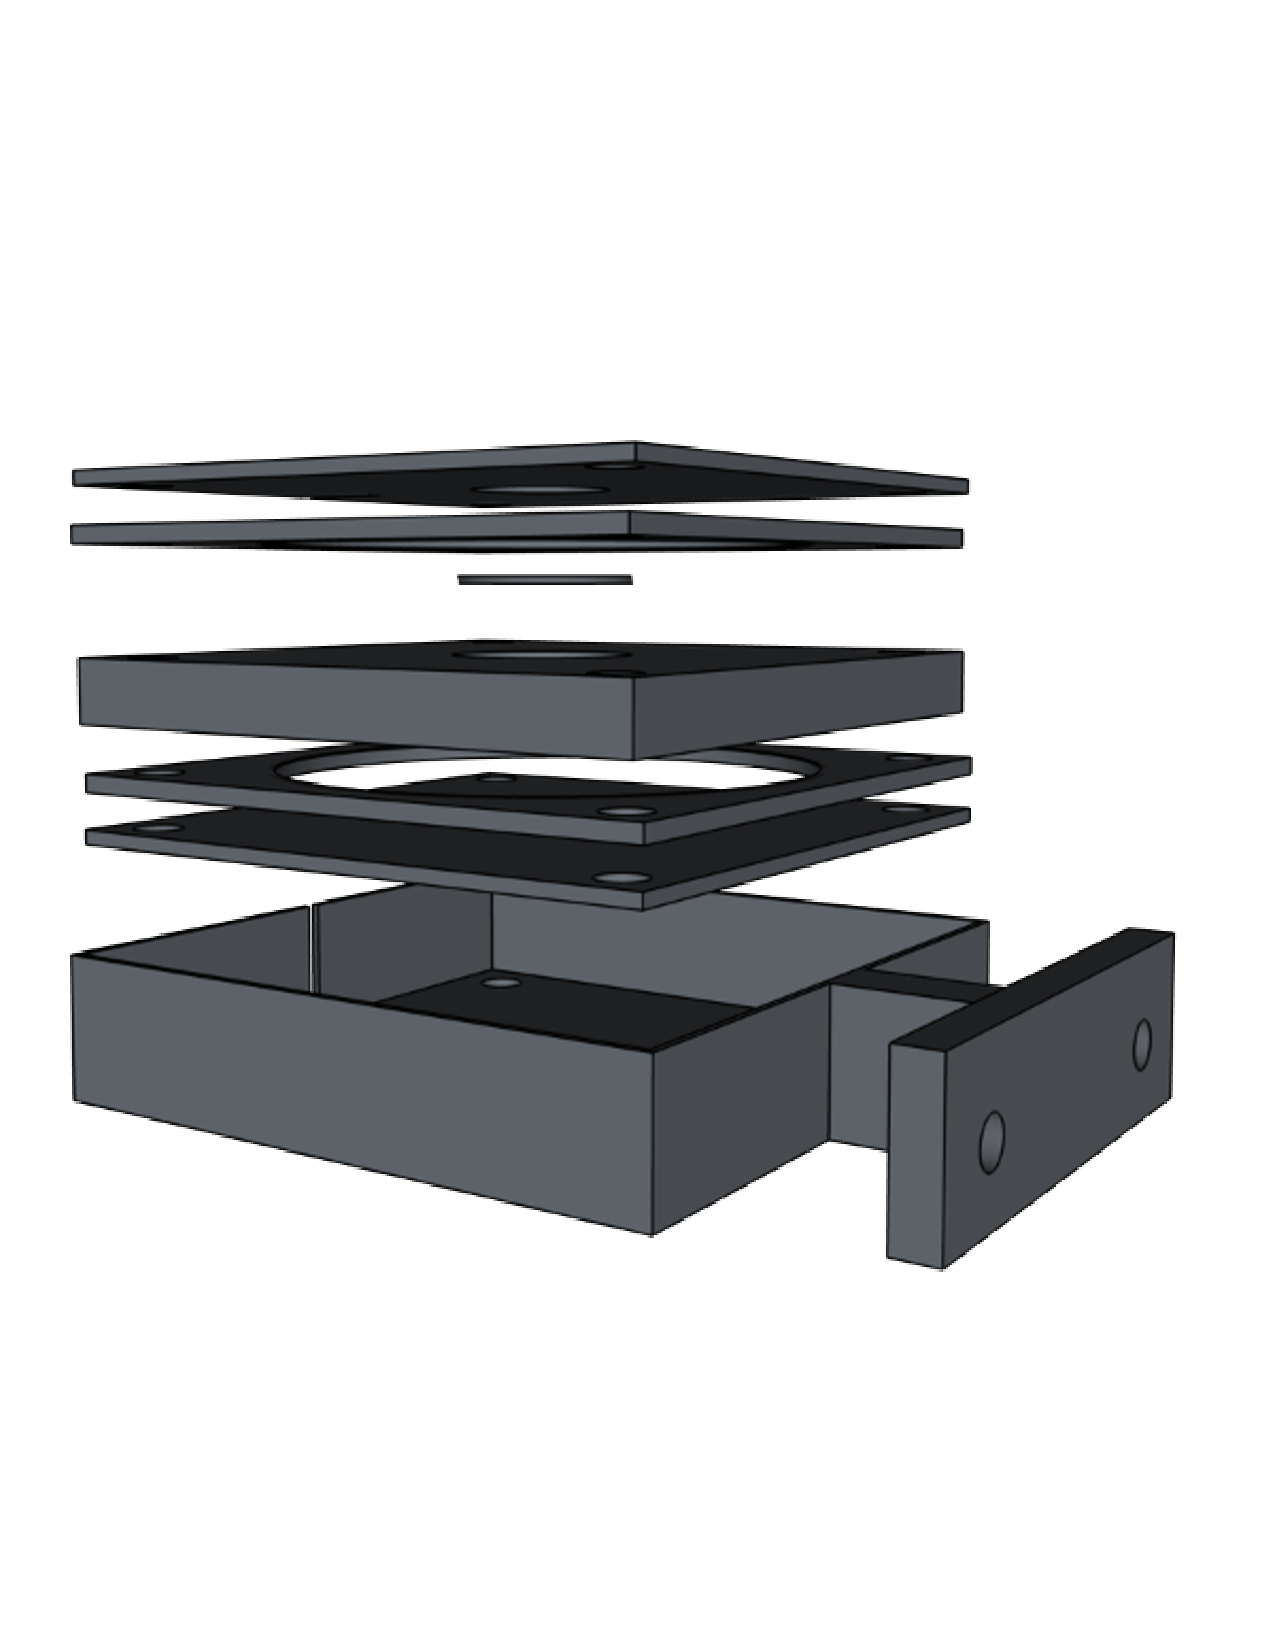
\includegraphics[width=.42\textwidth]{figs/ALGAAS/assemblies/assembly0/assembly0.pdf}
		\phantomcaption\label{A0}
		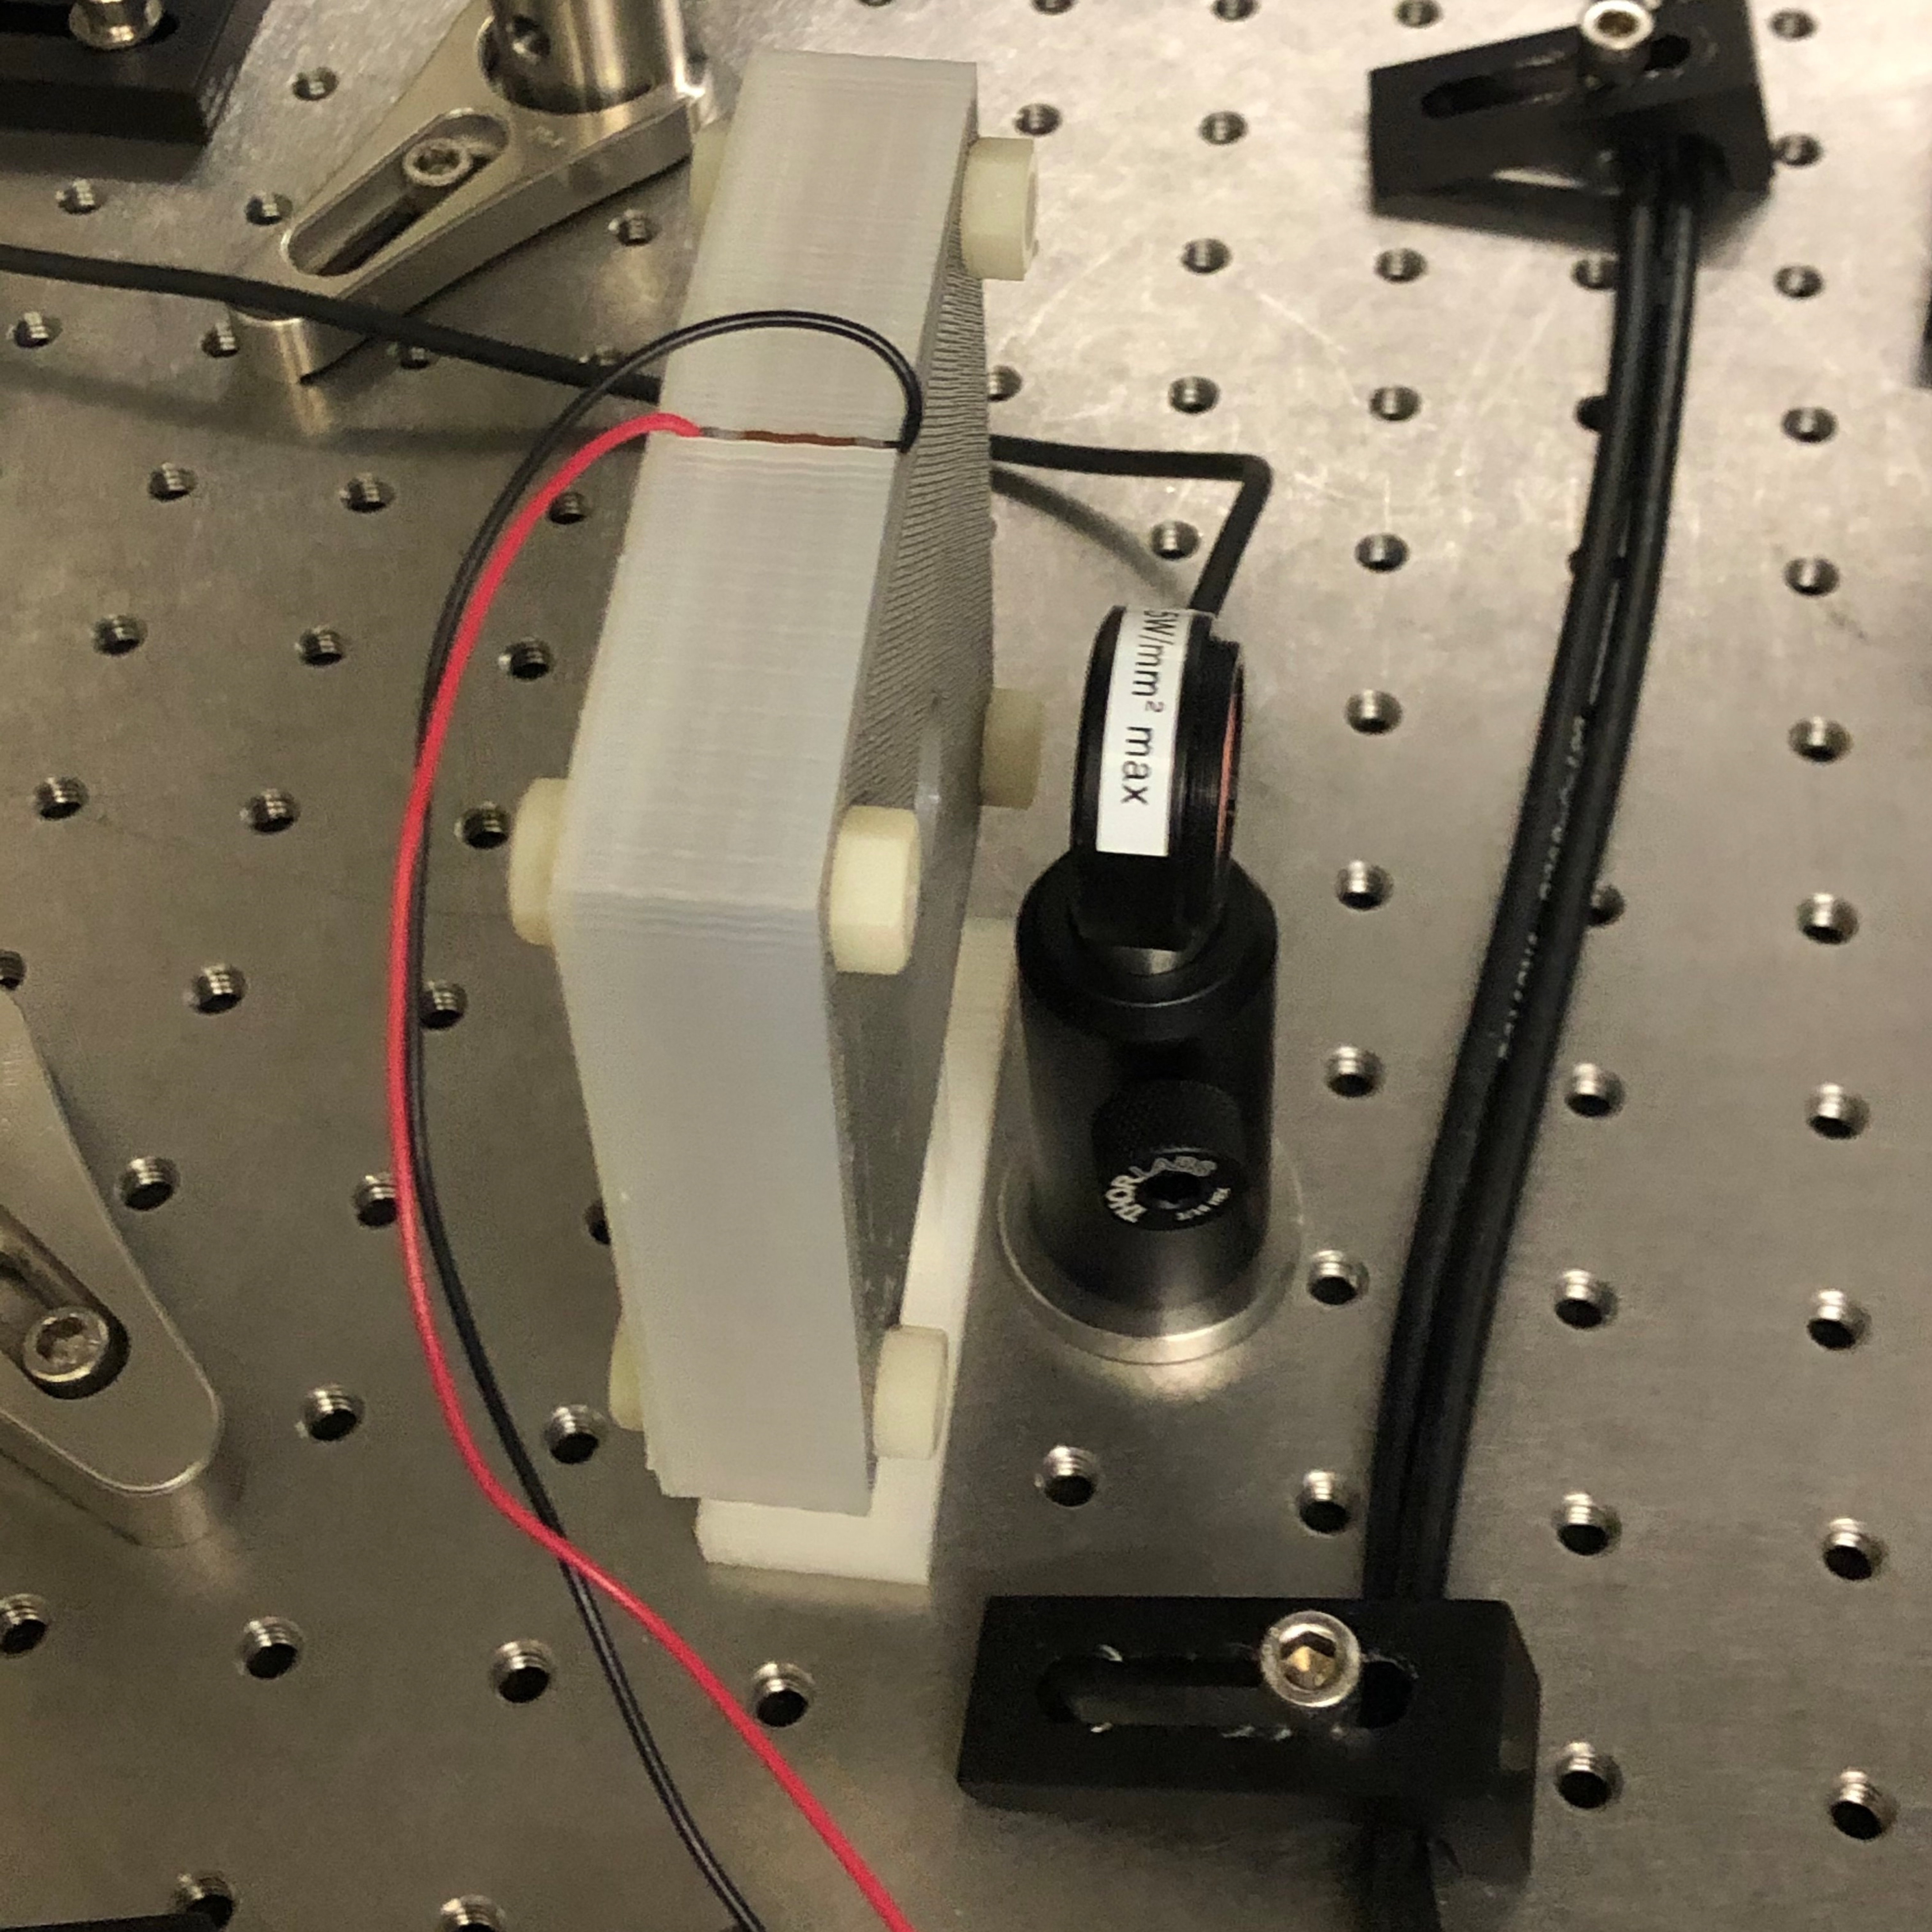
\includegraphics[width=.42\textwidth]{figs/ALGAAS/assemblies/assembly0/assembly0_incident_power.pdf}
 		\phantomcaption\label{A0inc}
	\end{subcaptiongroup}
  \caption{Assembly 0 was constructed to meet the criteria of providing a non-conductive housing for the electrode / sample assembly while maintaining a fixed length spacing using parts 3d printed with polylactic acid filament (PLA).}
  \label{fig:assembly0bp}
\end{figure}
\FloatBarrier
\subsubsection*{Mount 1.1}
\begin{figure}[!ht]
	\begin{subcaptiongroup}
		\centering
		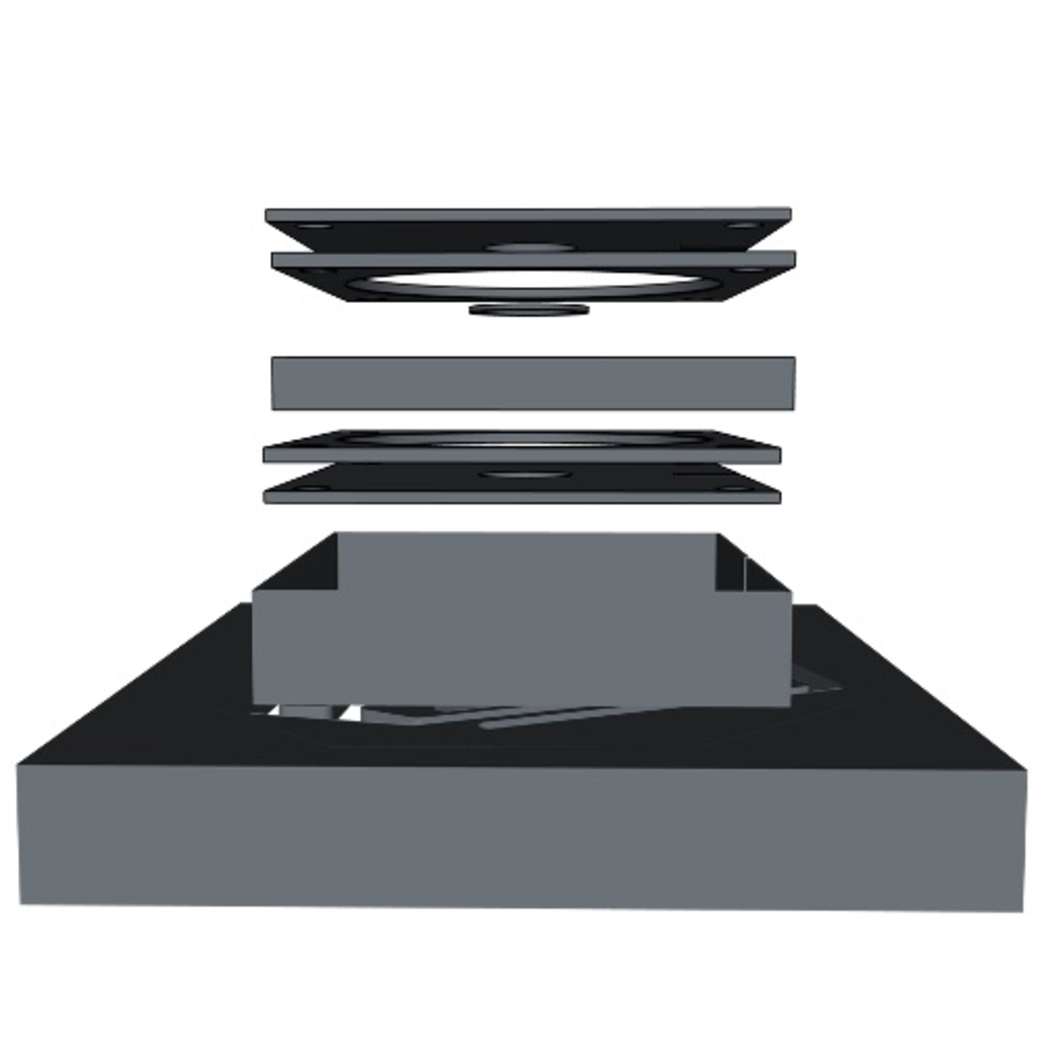
\includegraphics[width=.42\textwidth]{figs/ALGAAS/assemblies/assembly1/assembly1_dissassembled.pdf}
		\phantomcaption\label{A1pt2CAD}
		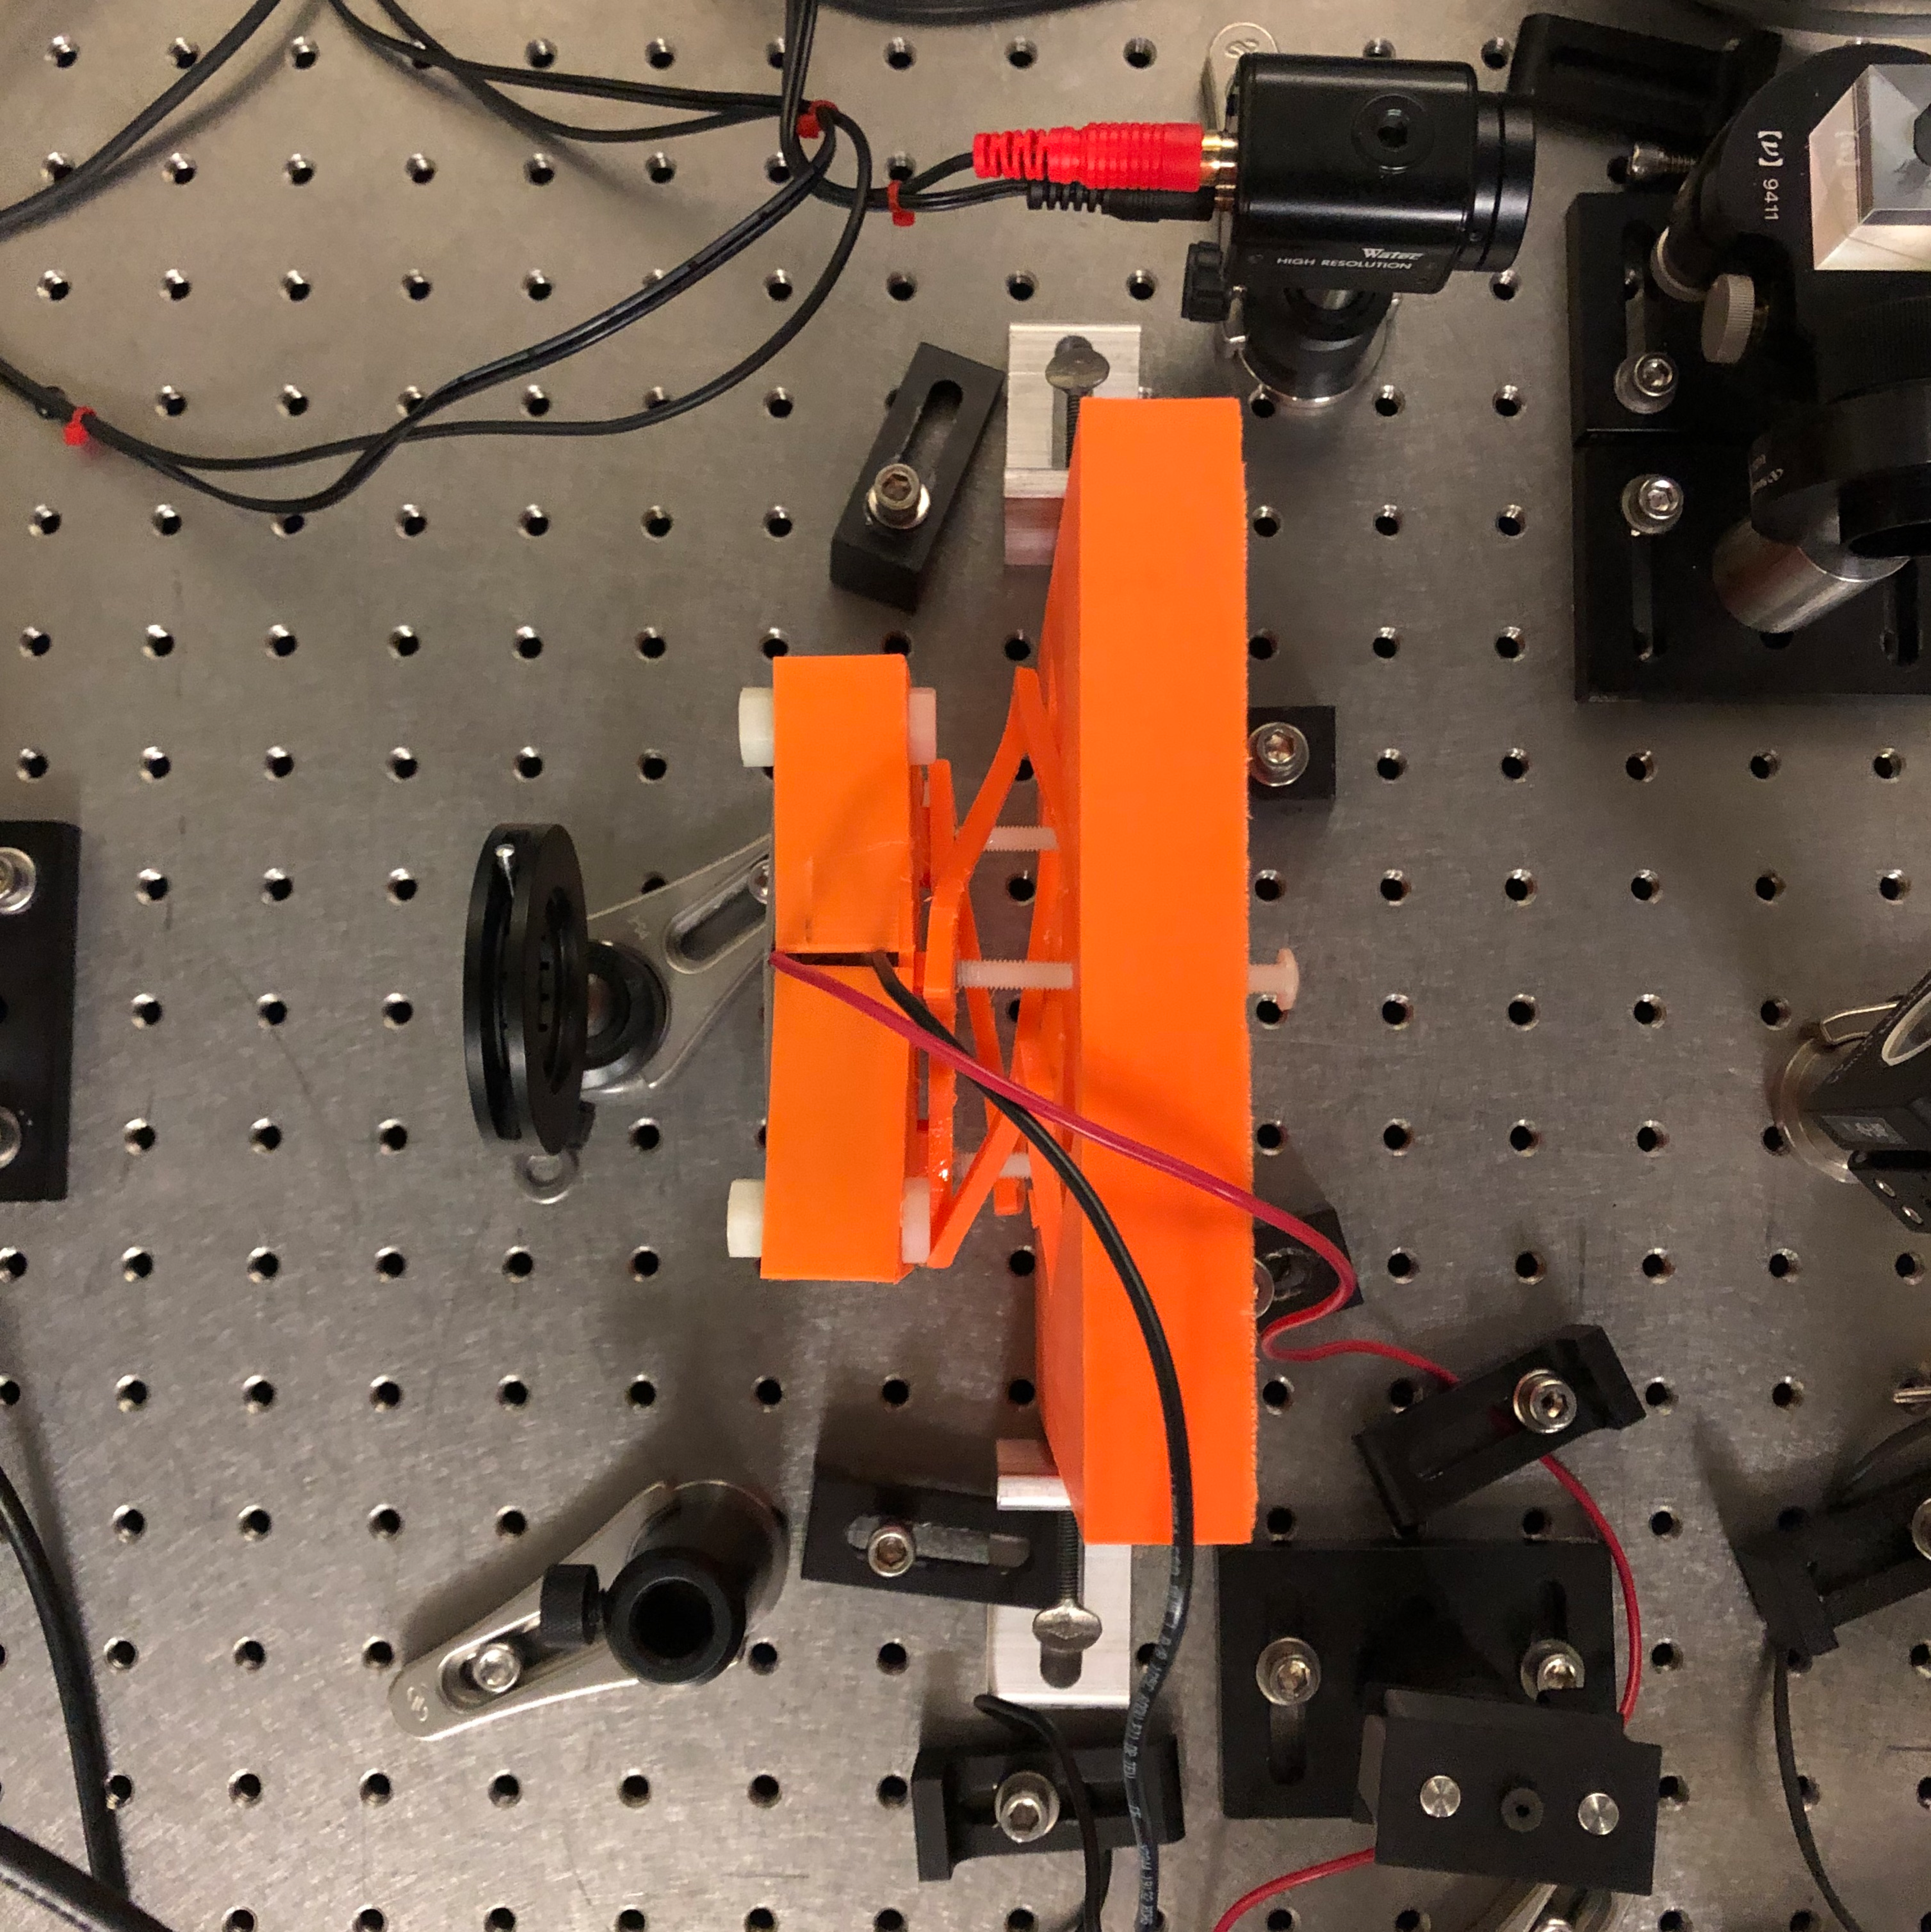
\includegraphics[width=.42\textwidth]{figs/ALGAAS/assemblies/assembly1/assembly1_insitu2.pdf}
		\phantomcaption\label{A1pt2pic}	
	\end{subcaptiongroup}
	\caption{Assembly 1 was constructed to meet the criteria of providing a non-conductive housing for the electrode / sample assembly while maintaining a fixed length spacing using parts 3d printed with polylactic acid (PLA). The assembly is coupled to an ortho-planar spring to allow for a built-in pitch/yaw control}
	\label{fig:assembly1bp}
\end{figure}
\FloatBarrier

\paragraph*{Mount 1.2}
\begin{figure}[!ht]
	\begin{subcaptiongroup}
		\includegraphics[width=.5\textwidth]{figs/ALGAAS/assemblies/assembly1/assembly1_mod_front.pdf}
		\phantomcaption\label{A1pt3CAD}
		\includegraphics[width=.5\textwidth]{figs/ALGAAS/assemblies/assembly1/assembly1_mod_side.pdf}
		\phantomcaption\label{A1pt3pic}
	\end{subcaptiongroup}
	\caption{A modification implemented with the intention of reducing pitch dithering while still having control of DC YAW}
	\label{fig:assembly1mod}
\end{figure}
\newpage

\subsubsection{Assembly 2}
\paragraph*{Model Params}
\begin{center}
\begin{tabular}{ |c|c|c|c|c|c| } 
\hline
$\mathrm{r}_{ap}$ [m] &  $\mathrm{t}_{cap}$ [m] & $\mathrm{r}_{el}$ [m] & $\mathrm{t}_{el}$ [m] & $\mathrm{r}_{opt}$ [m] & $\mathrm{t}_{opt}$ [m] \\
\hline
1.5e-3 & 12.7e-3 & N/A (rectangular) & 1.27e-3 & 12.7e-3 & 6.35e-3 \\ 
\hline
\end{tabular}
\end{center}

\paragraph*{Electrodes}

\begin{figure}[H]
  \centering
  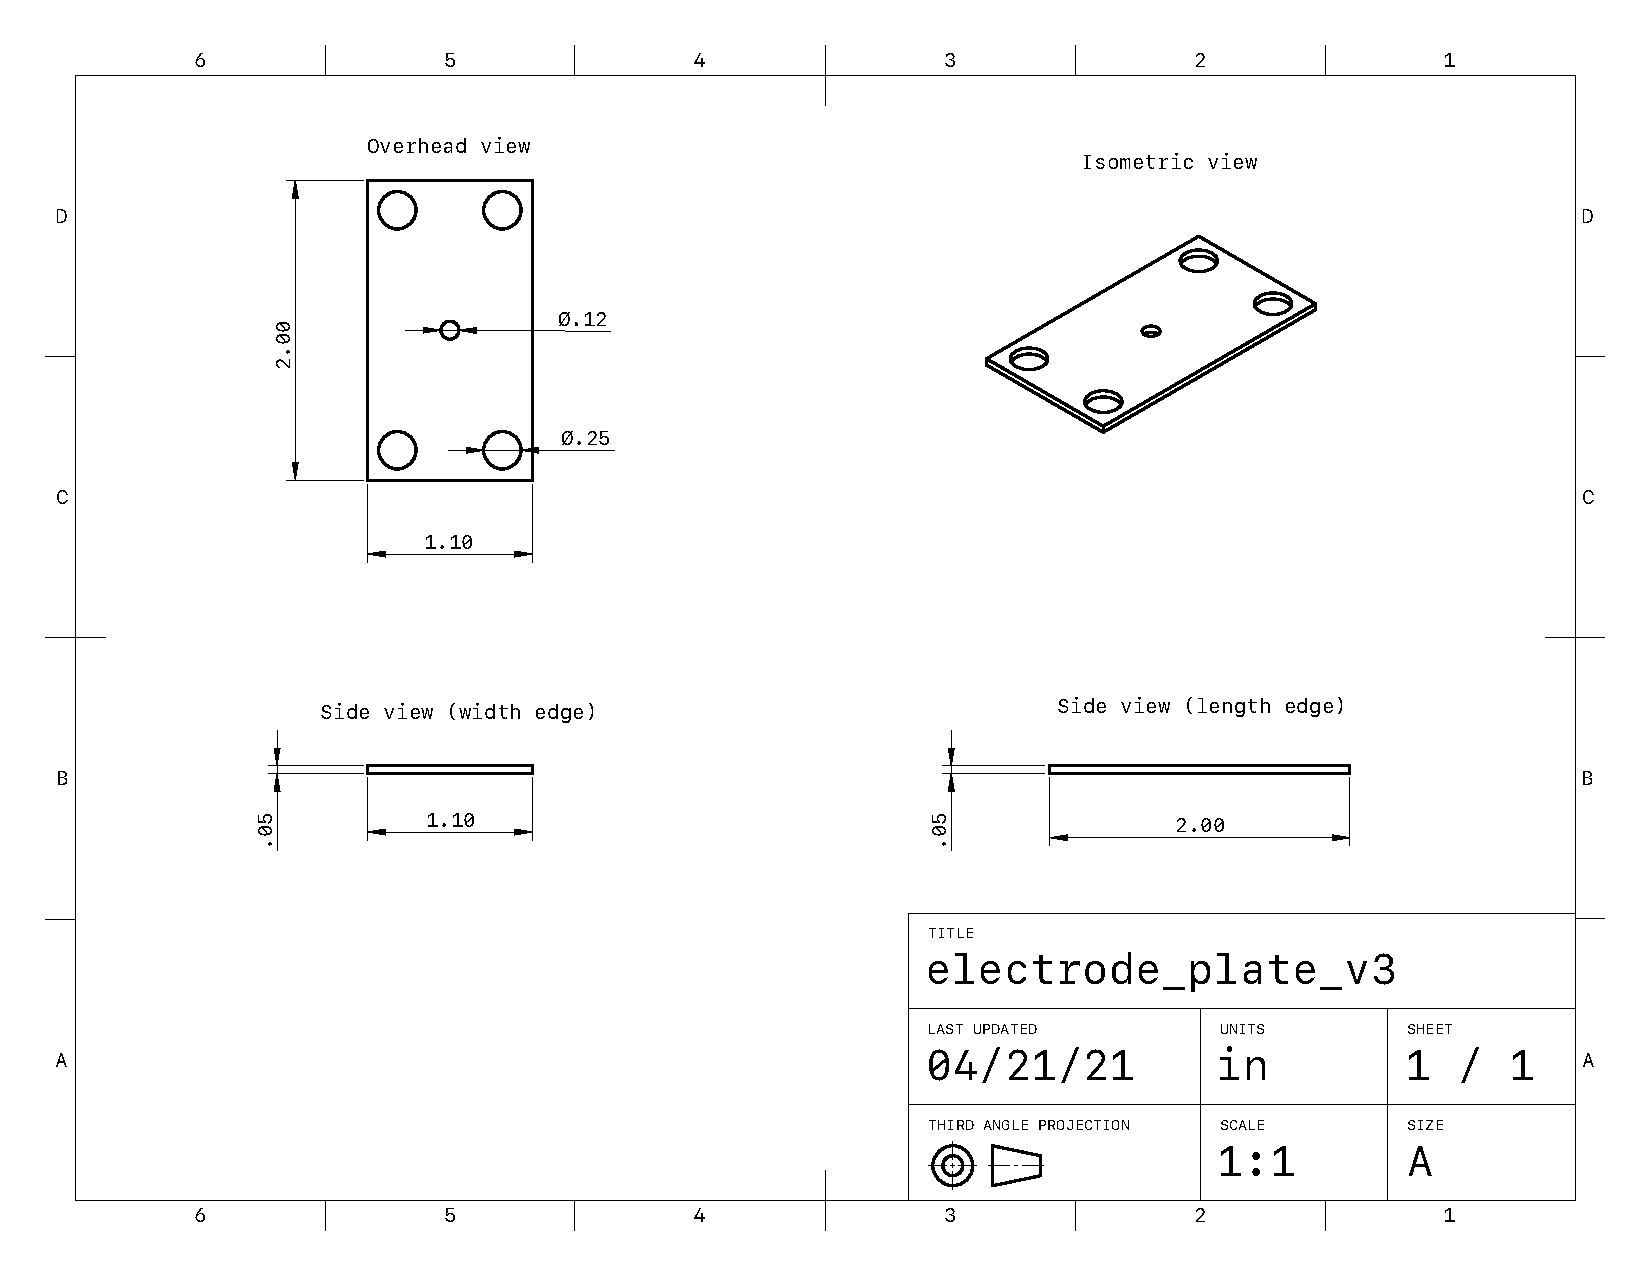
\includegraphics[width=\textwidth]{figs/ALGAAS/assemblies/assembly2/assembly2_electrode.pdf}
  \caption{Rectangular (.05"X1.1"X2") plates made of aluminum.}
\end{figure}

\newpage

\paragraph*{Mount 2.0}
\begin{figure}[H]
	\centering
	\begin{subcaptiongroup}
		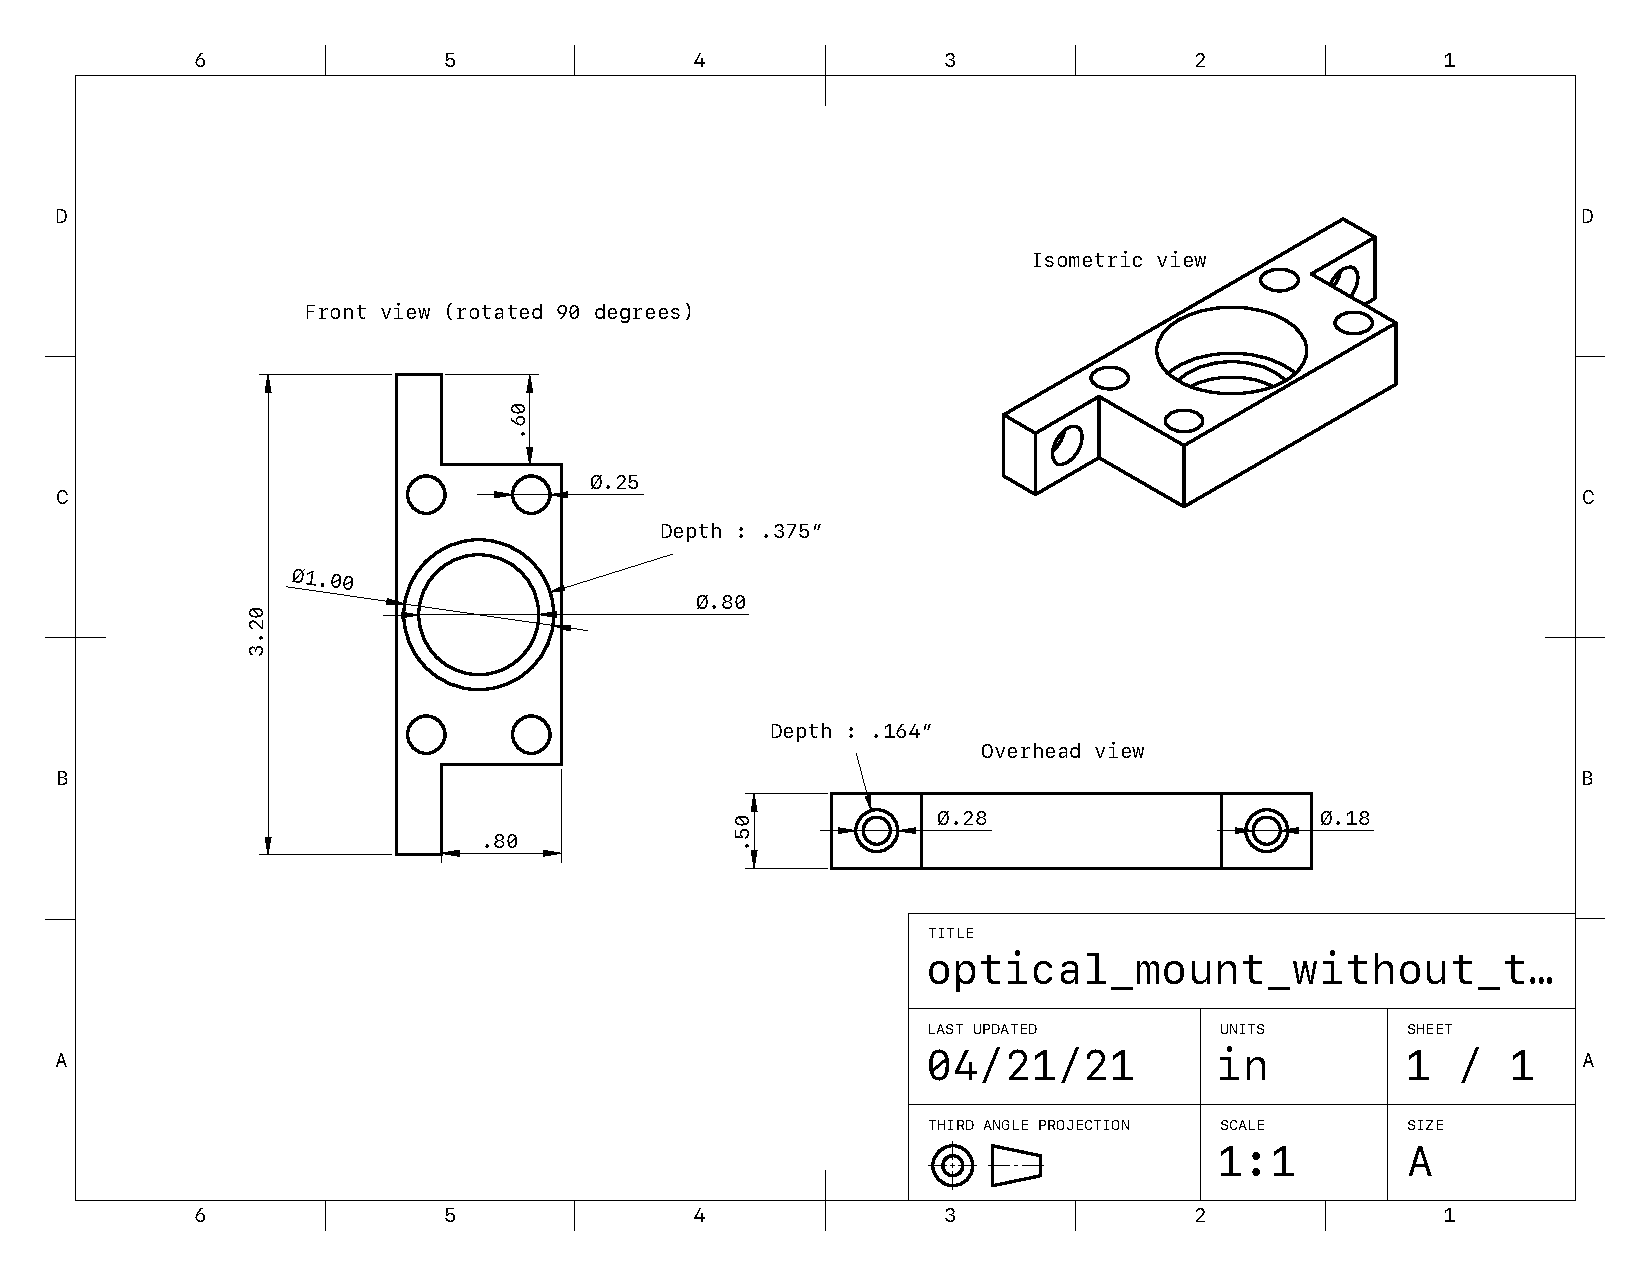
\includegraphics[width=.76\textwidth]{figs/ALGAAS/assemblies/assembly2/assembly2_PVC_mount.pdf}
		\phantomcaption\label{A2PVCmount}
		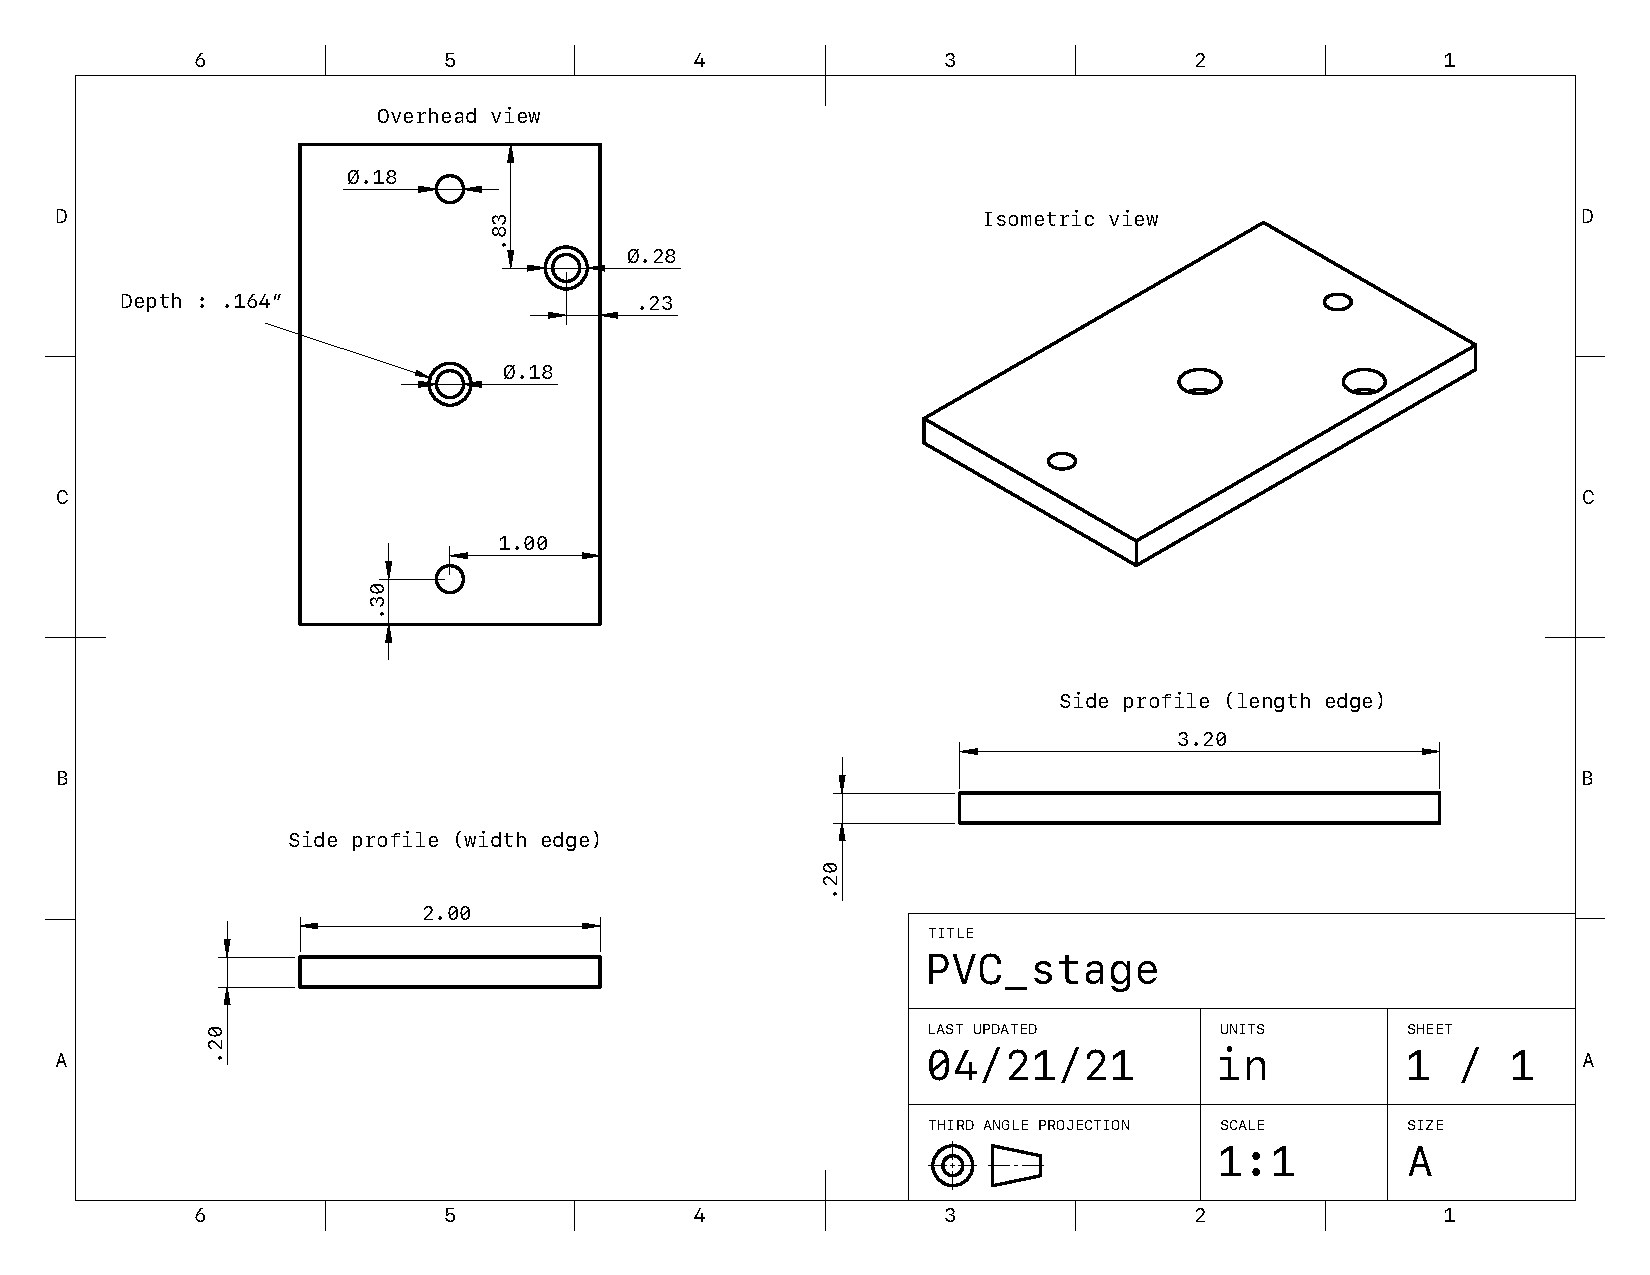
\includegraphics[width=.76\textwidth]{figs/ALGAAS/assemblies/assembly2/assembly2_PVC_stage.pdf}
		\phantomcaption\label{A2PVCstage}
	\end{subcaptiongroup}
	\caption{A design iteration of the assembly 2 mounts. Materials tried varied from PVC, PLA, and PETG. Quarter inch holes are bored in order to pass nylon screws holding electrode plates fixed to the mount.}
	\label{fig:assembly2bp}
\end{figure}
\FloatBarrier

Varying the mechanical configurations (i.e. differential electrode and / or optic set screw settings) to the slightest degree left us to discover a variety of drive couplings via excitations from the assembly sample-mount acoustic modes while driving the voltage on electrodes plates. Tracking consistent mechanical response for assemblies prior to Assembly 3 proved challenging due to inconsistent mechanical settings between some measurements and span different geometries / material properties. An adequate solution was dependent on selecting a material and geometry that would generate narrow acoustic resonances while simultaneously achieving adequately low noise within a bandwidth of interest (a not so uncommon experimental technique, esp. for optic suspensions, that is frequently used and mentioned within collaboration literature). Assembly 3 demonstrated such characteristics and is discussed further.
\newpage
\subsubsection{Assembly 3 (MACOR mount)}

\paragraph*{Model Params}
\begin{center}
\begin{tabular}{ |c|c|c|c|c|c| } 
\hline
$\mathrm{r}_{ap}$ [m] &  $\mathrm{t}_{cap}$ [m] & $\mathrm{r}_{el}$ [m] & $\mathrm{t}_{el}$ [m] & $\mathrm{r}_{opt}$ [m] & $\mathrm{t}_{opt}$ [m] \\
\hline
1.5e-3 & 6.94e-3 & 15.75e-3 & 9.66e-3 & 12.7e-3 & 6.35e-3 \\ 
\hline
\end{tabular}
\end{center}

\paragraph*{Electrodes}
\begin{figure}[H]
  \centering
  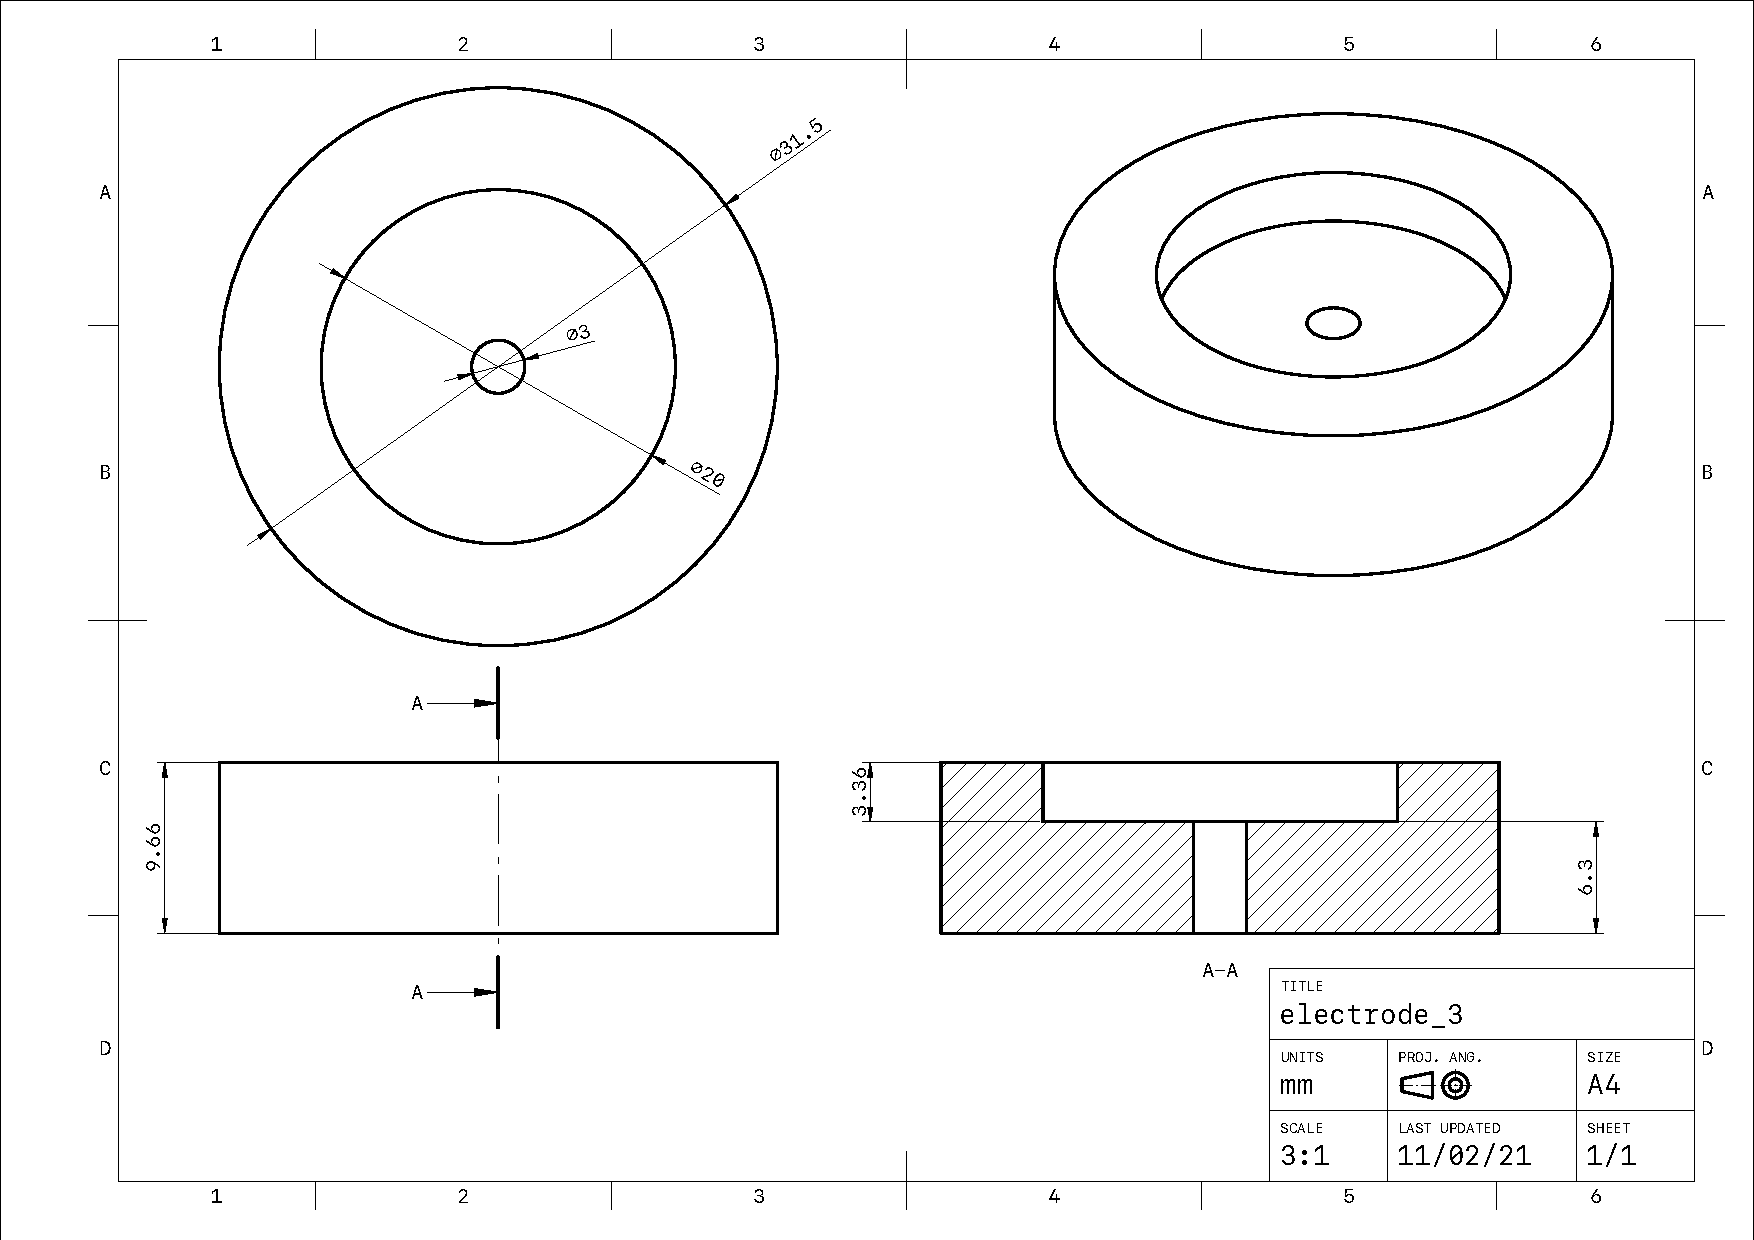
\includegraphics[width=.6\textwidth]{figs/ALGAAS/assemblies/assembly3/electrode_3.pdf}
  \caption{Technical drawing of thick disk electrode plates made of copper.}
\end{figure}

\paragraph*{Mount 3.0}

\begin{figure}[H]
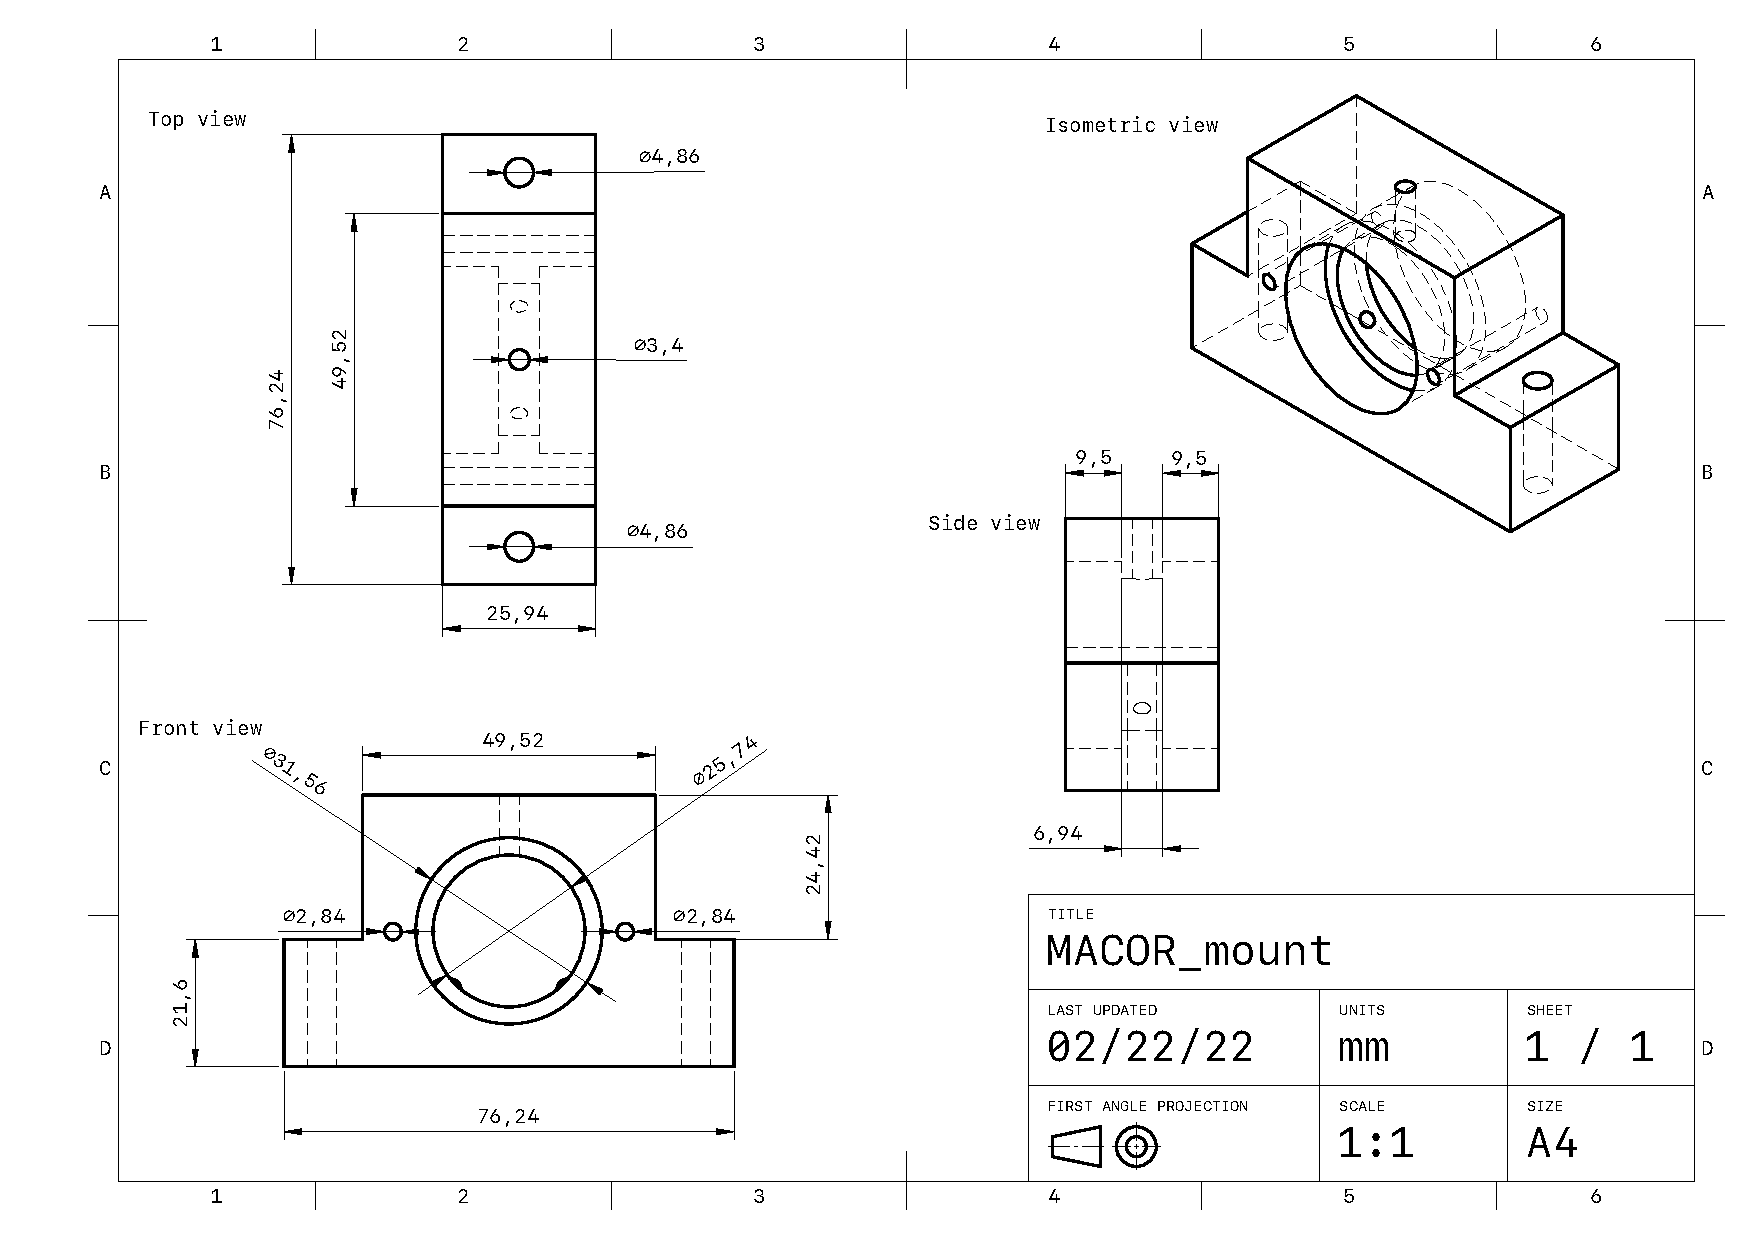
\includegraphics[width=\textwidth]{figs/ALGAAS/assemblies/assembly3/MACOR_mount.pdf}
\caption{MACOR mount design constucted in Shapr3D}
\label{fig:macormountdesign}
\end{figure}

To maintain the aforementioned \hyperlink{fig:laplacecoords}{boundary conditions} in situ, an optical mount made of MACOR, a machinable ceramic, was built and installed. With the material's high Young's modulus (66.9 GPa), and a moderate Poisson ratio (.29) \cite{macor} making it by far the most durable / non-conductive mounting solution tried.

An optical mount for the sample made with MACOR, along with spherical glass bearnings with a .48 $\pm$ .01 cm $\diameter$, and a McMaster-Carr 8-32, 1/2" ceramic screw were used to clamp the optical sample within a bored 25.74 $\pm$ .5 mm $\diameter$ barrel. Two 1.24" $\diameter$ holes were also bored at a 9 mm depth about the front and back side of the optical mount to accomodate for a flush fit of copper electrodes. The construction suggests a 1 $\pm$ .5 mm clearance between the front and back surface of the sample to the electrode plates.

\begin{figure}[!ht]
    \centering
    \begin{subcaptiongroup}
	    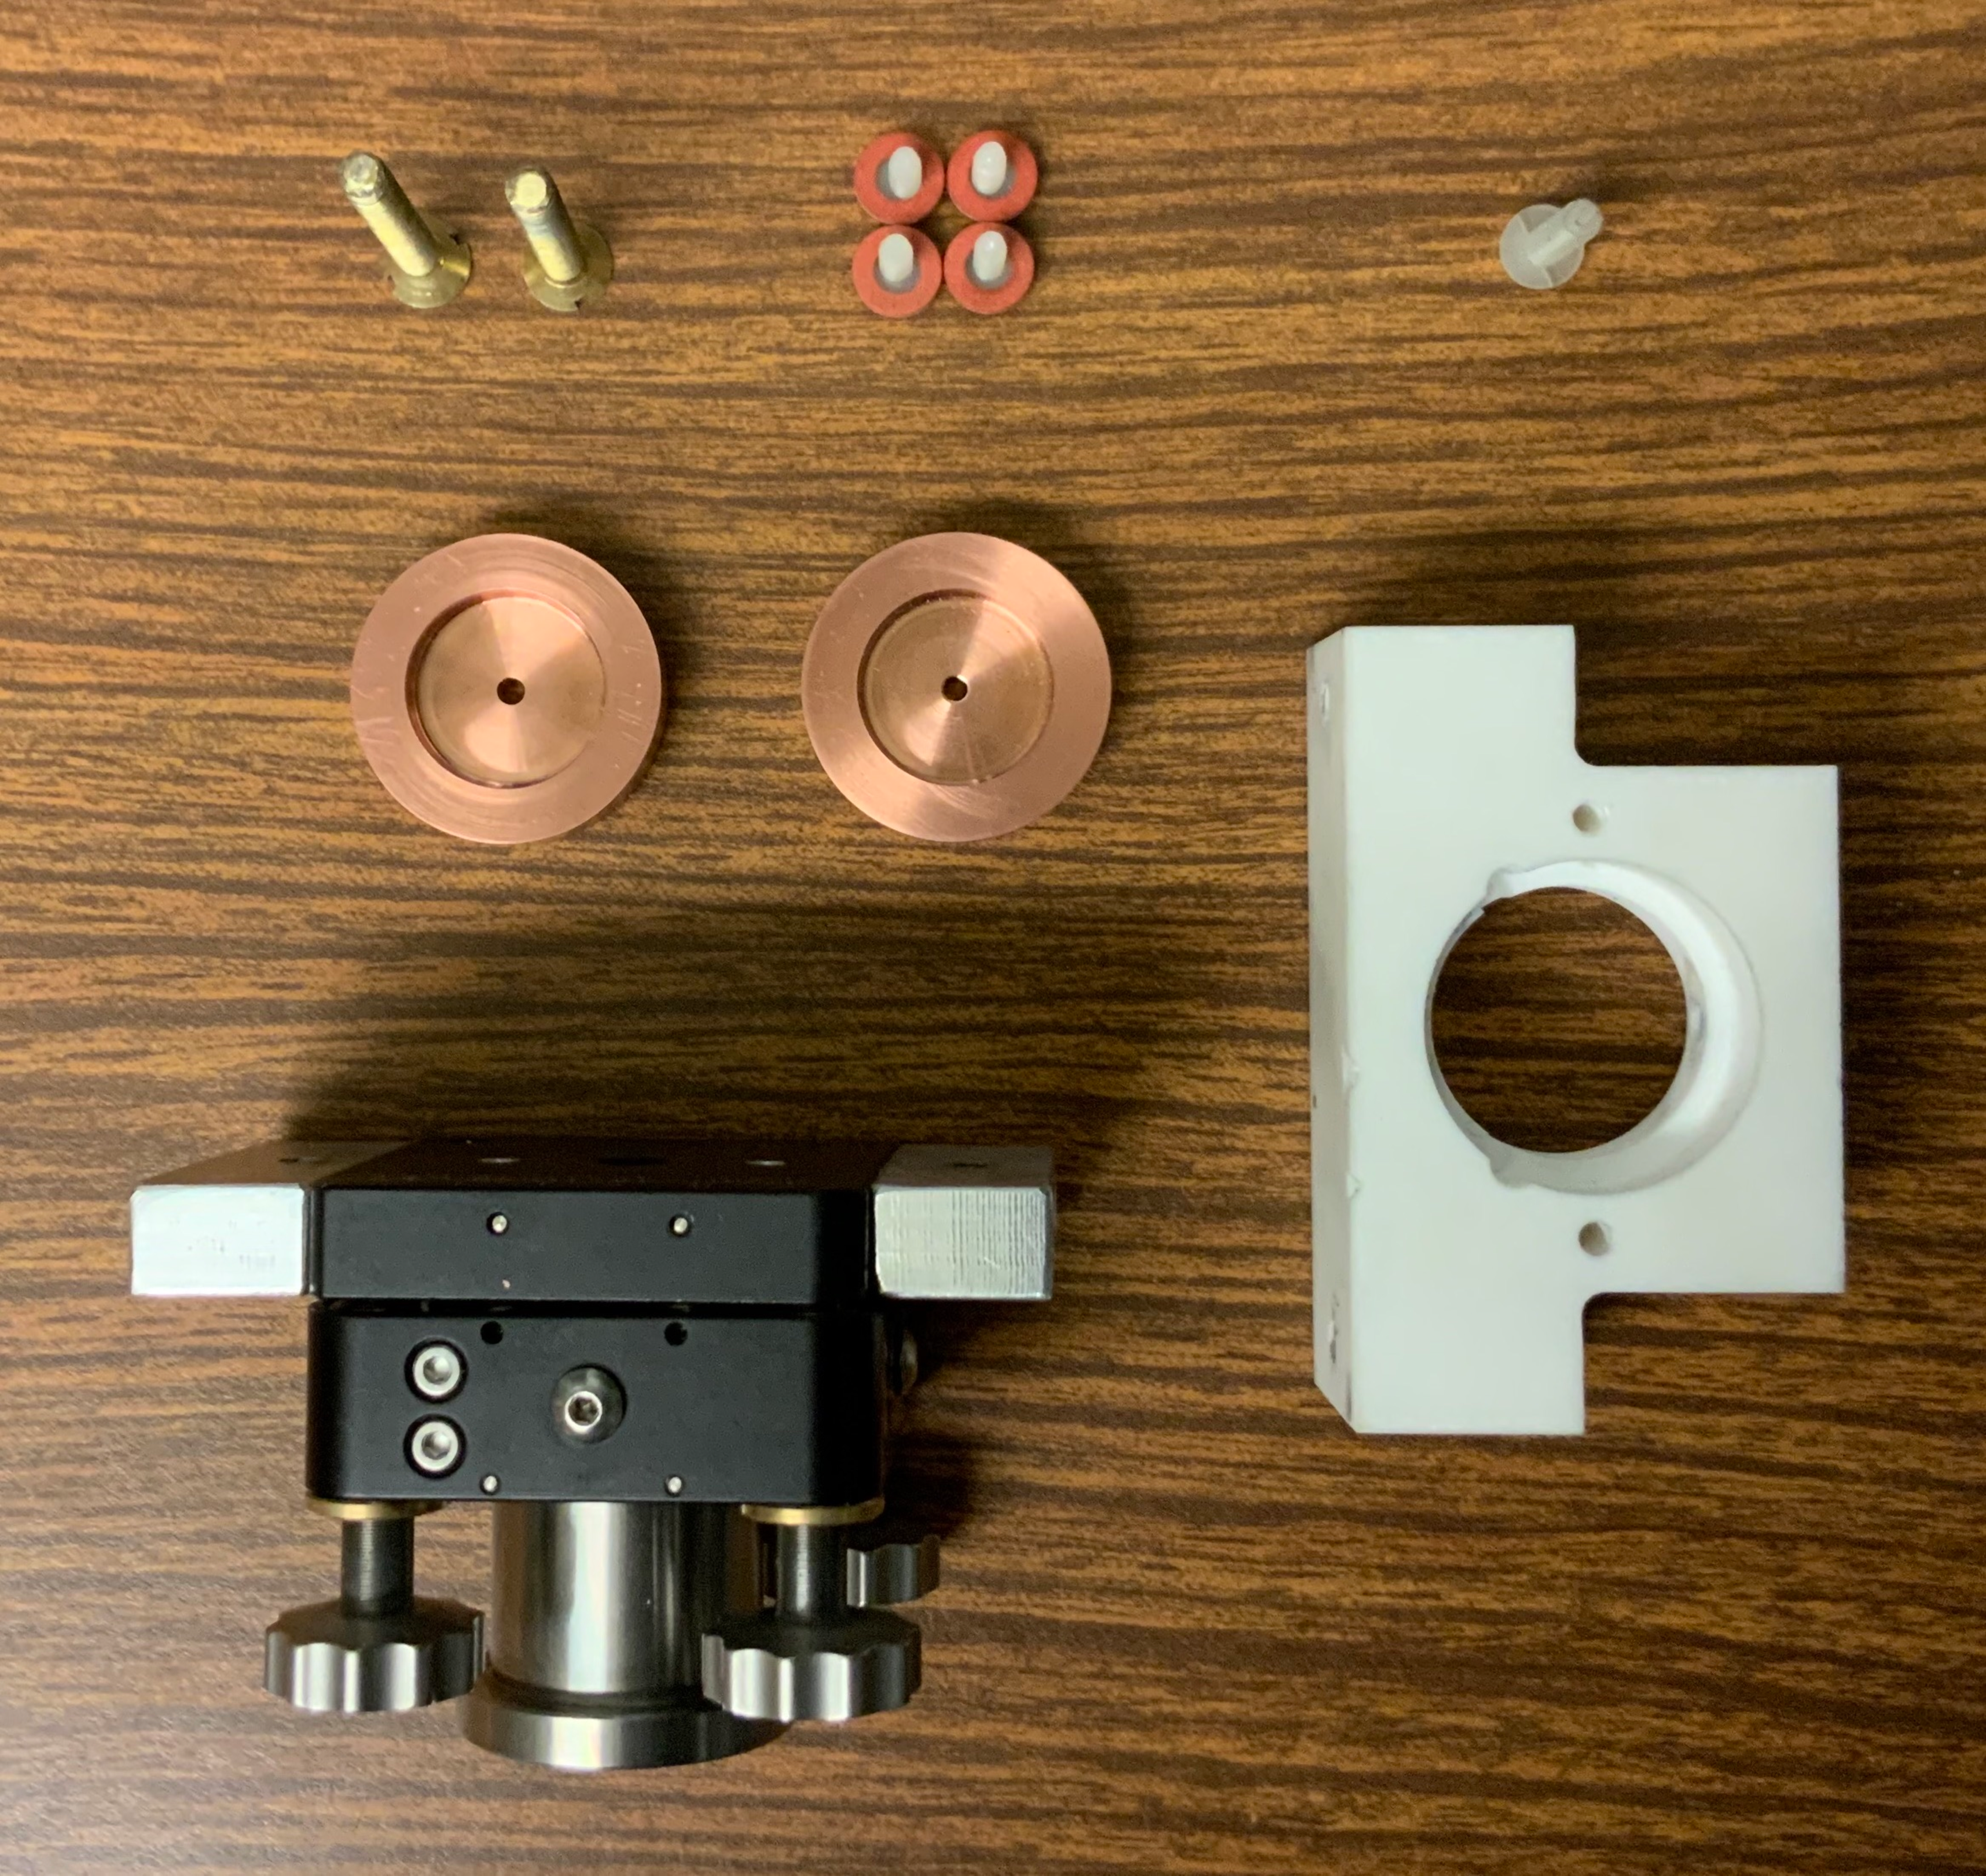
\includegraphics[width=.40\textwidth]{figs/ALGAAS/assemblies/assembly3/assembly3_disassembled.pdf}
	    \phantomcaption\label{subfig:A3disassembled}
	    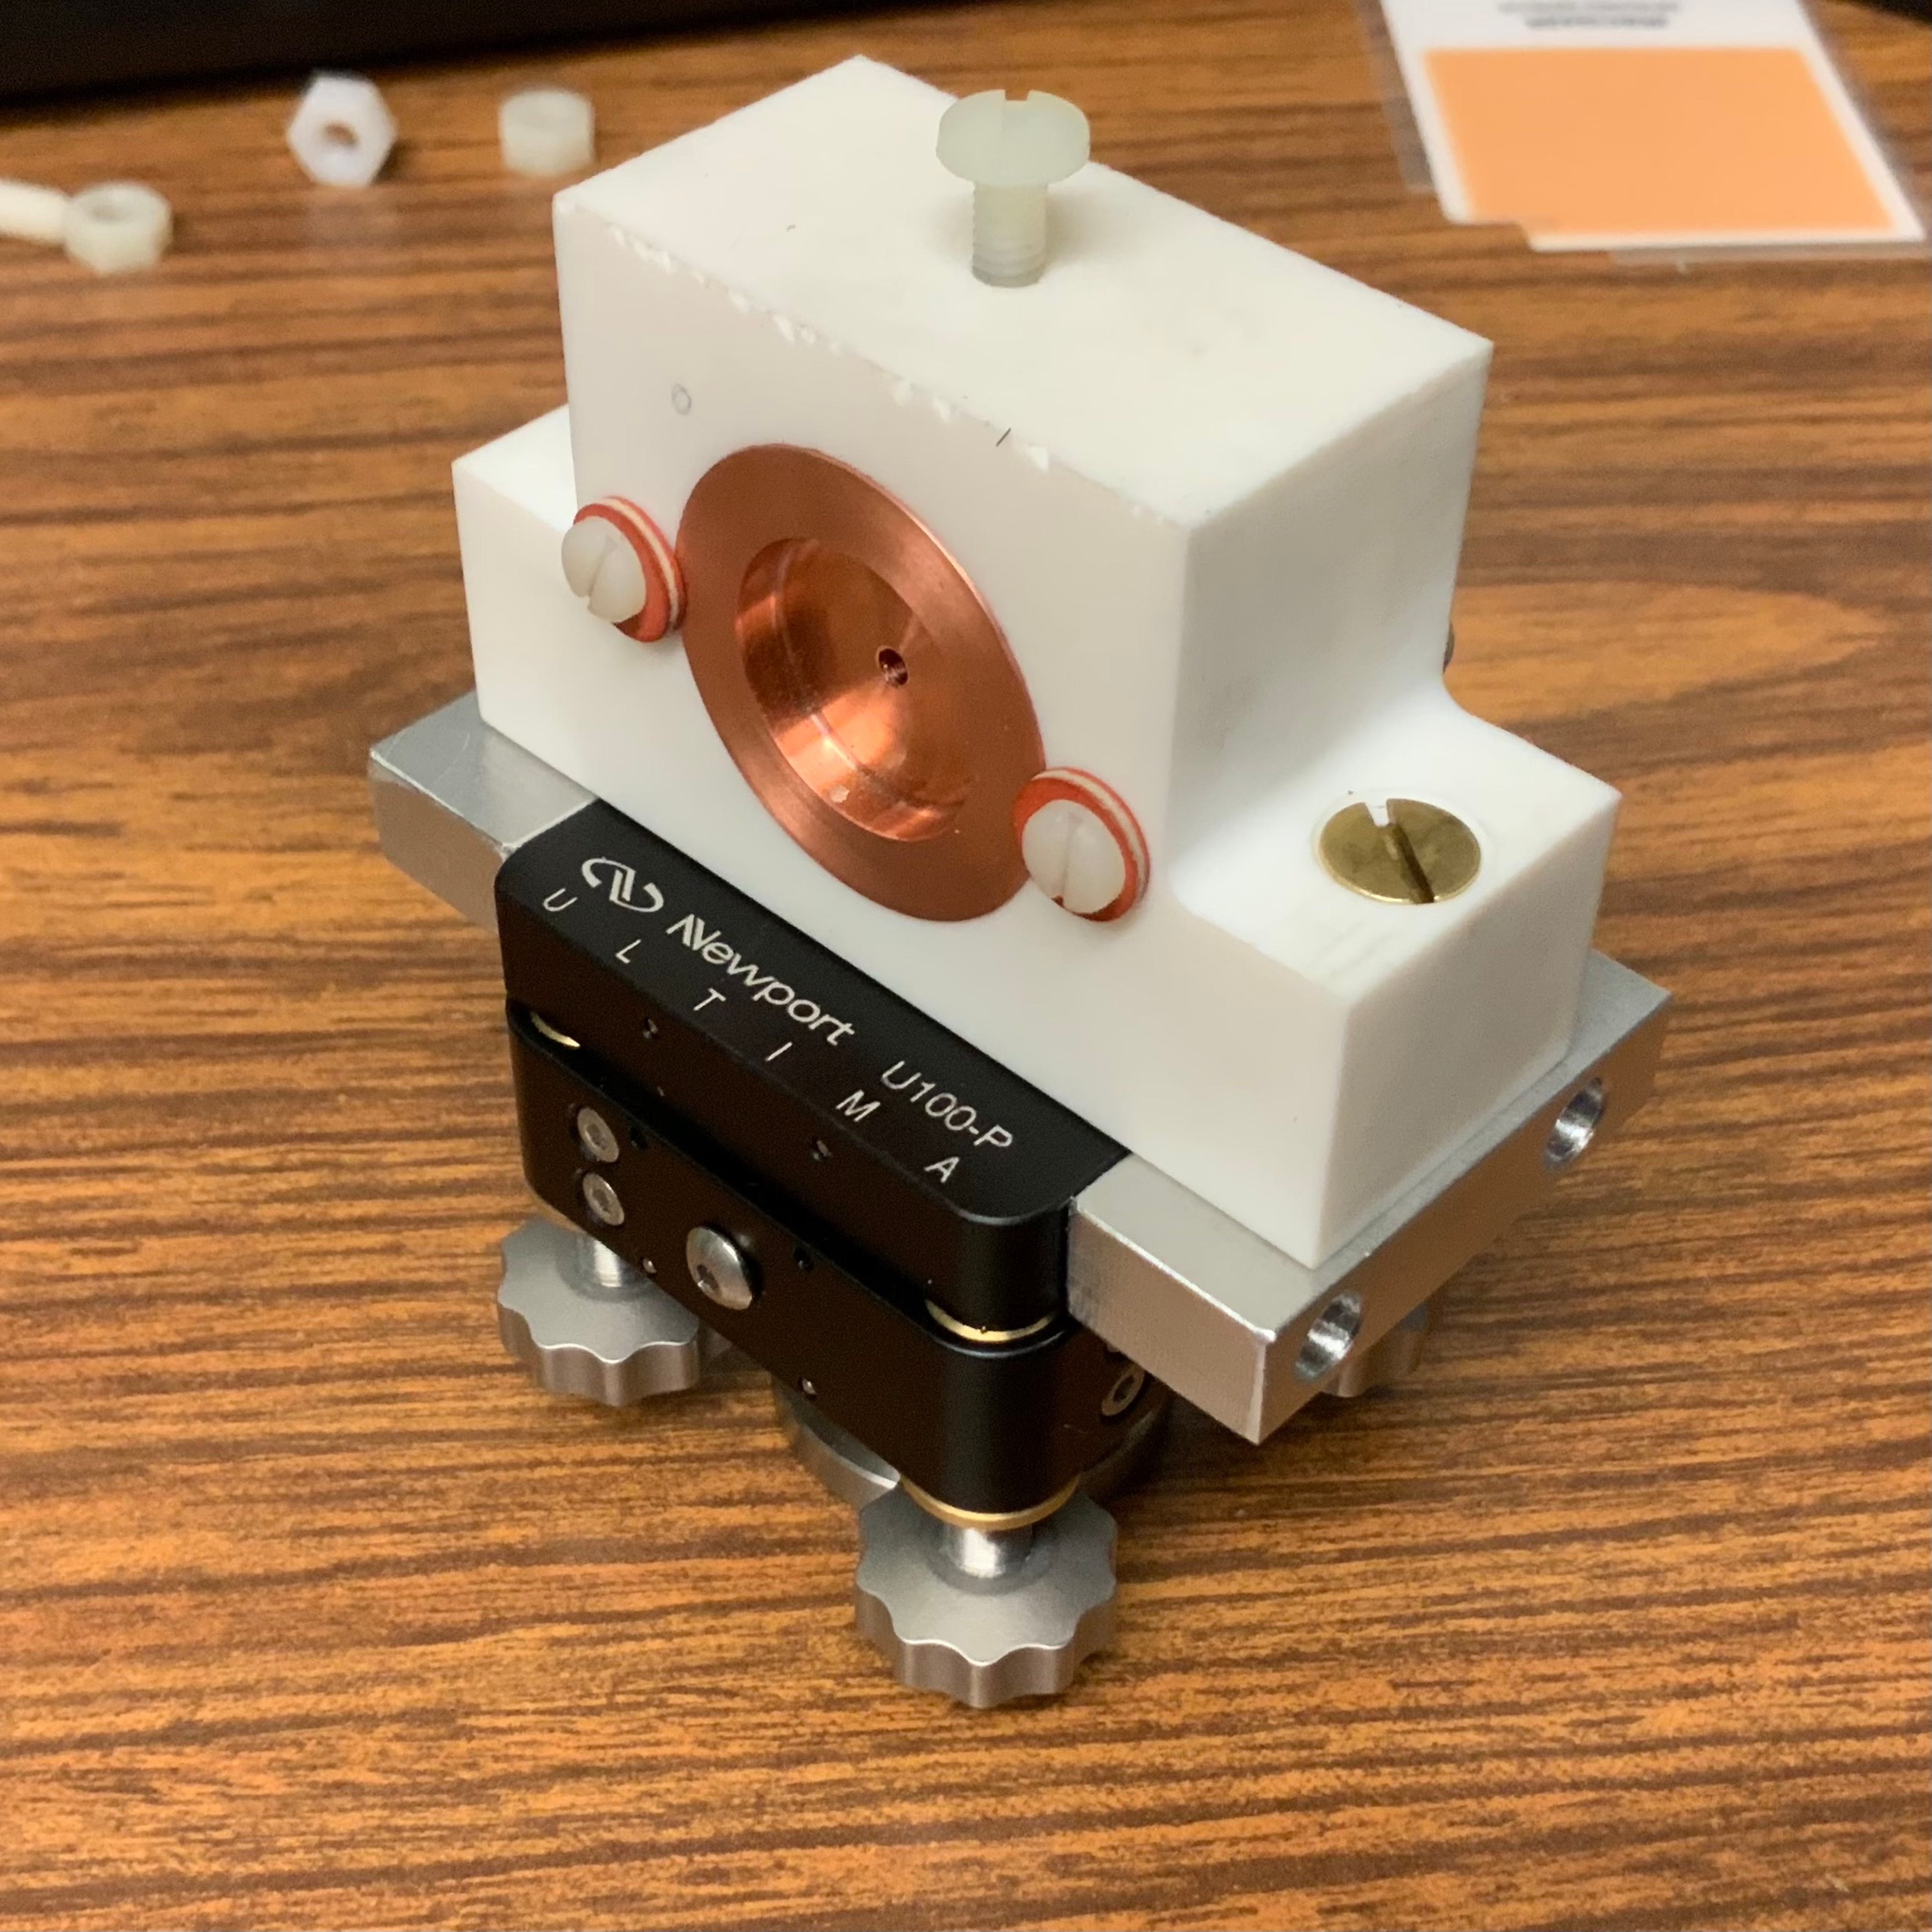
\includegraphics[width=.3776\textwidth]{figs/ALGAAS/assemblies/assembly3/assembly3_isometric.pdf}
	    \phantomcaption\label{subfig:A3isometric}
    \end{subcaptiongroup}
    \caption{Assembly 3: [Left] disassembled configuration and [Right] an isometric view of the assembled configuration. The electrodes initially used were made of copper; a material chosen its high density with the intention of combatting intertial influence at high frequency, though aluminum plates with near identical geometry were used for later results.}
    \label{fig:assembly3}
\end{figure}

\iffalse
\begin{figure}[H]
    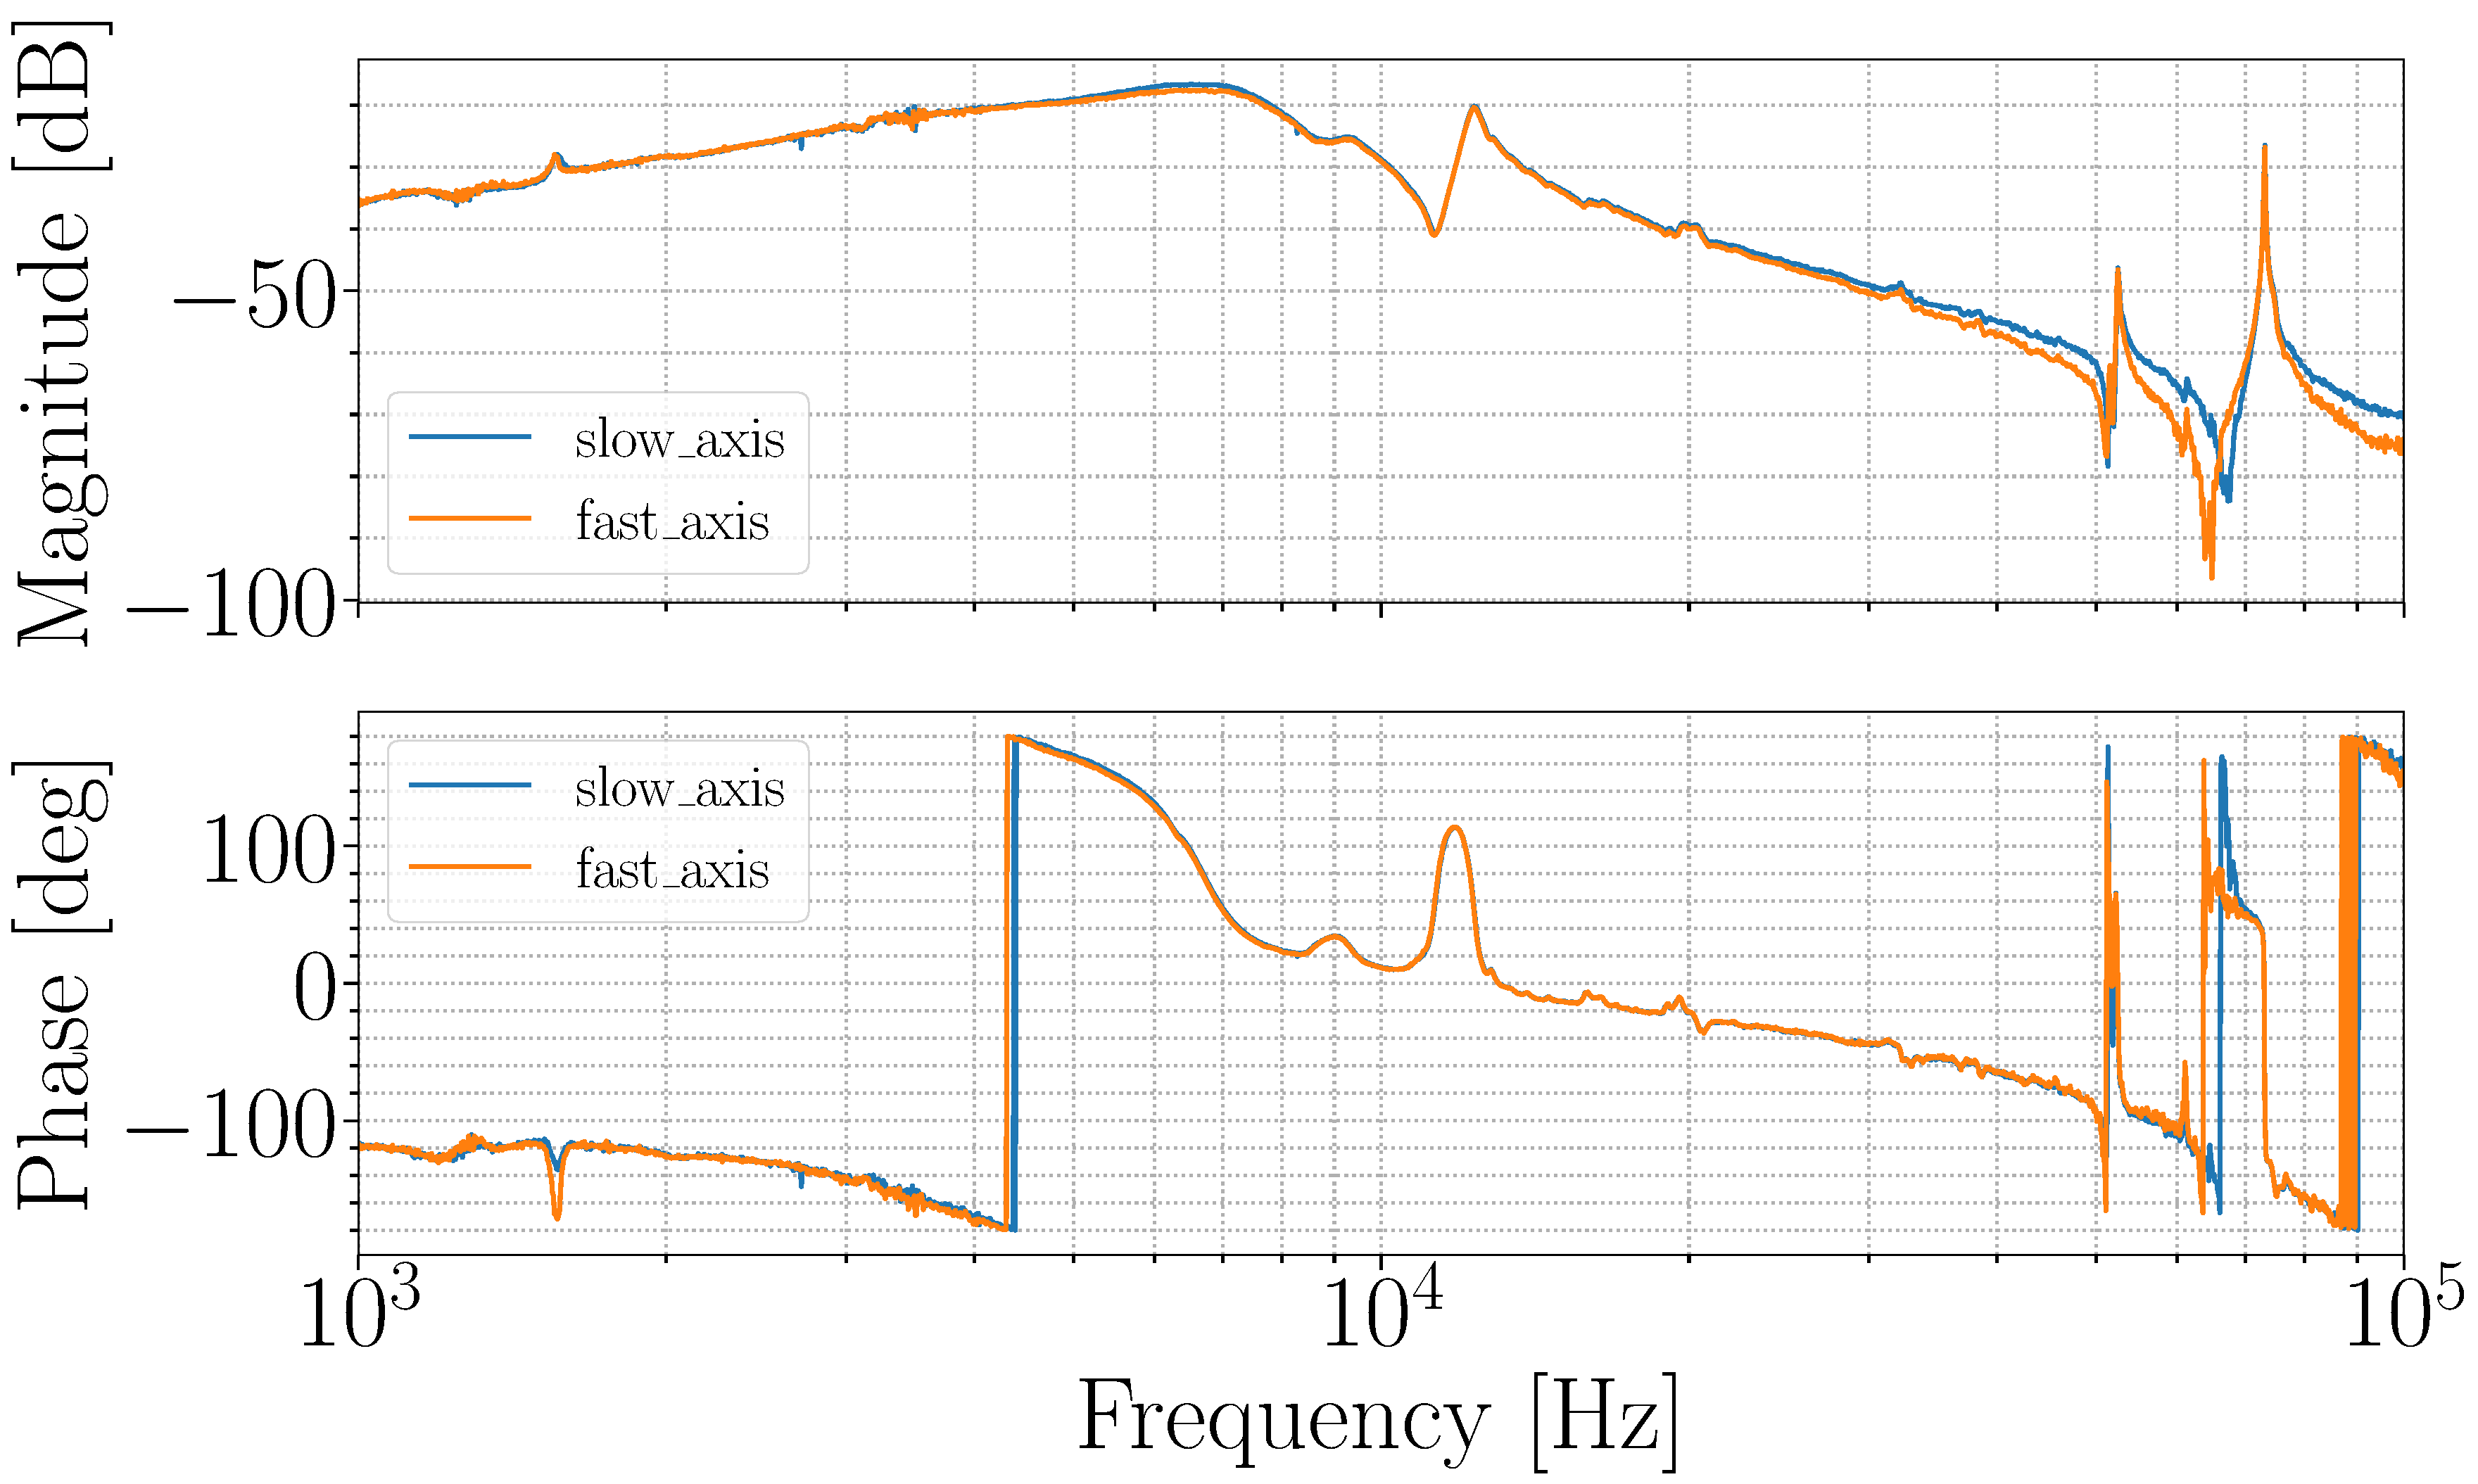
\includegraphics[width=\textwidth]{figs/ALGAAS/rawtf_fast_slow.pdf}
    \caption{Uncalibrated measurement with the polarization aligned along the slow and fast $\gaas$ / $\algaas$ coating axes using the MACOR mount}
    \label{fig:rawtf_fast_slow}
\end{figure}
\fi

This mount assembly lead to the published results discussed in the next chapter.

\iffalse
\subsection{Measured birefringence from HR \texorpdfstring{$\gaas$}{gaas}/\texorpdfstring{$\algaas$}{algaas} mirror}

To identify the fast and slow axes, the crystalline HR mirror is temporarily paired with a highly reflective input mirror to form a high finesse cavity. The DC power in reflection of the cavity was probed while the laser frequency was linearly swept about resonance and various input laser polarizations sampled using a half waveplate ($\lambda$ / 2). The resulting measurements exhibit a split cavity resonance when the beam polarization is not co-aligned with one of the two eigenaxes set by the HR sample birefringence.

\begin{figure}
    \centering
    \begin{subfigure}{.48\linewidth}
	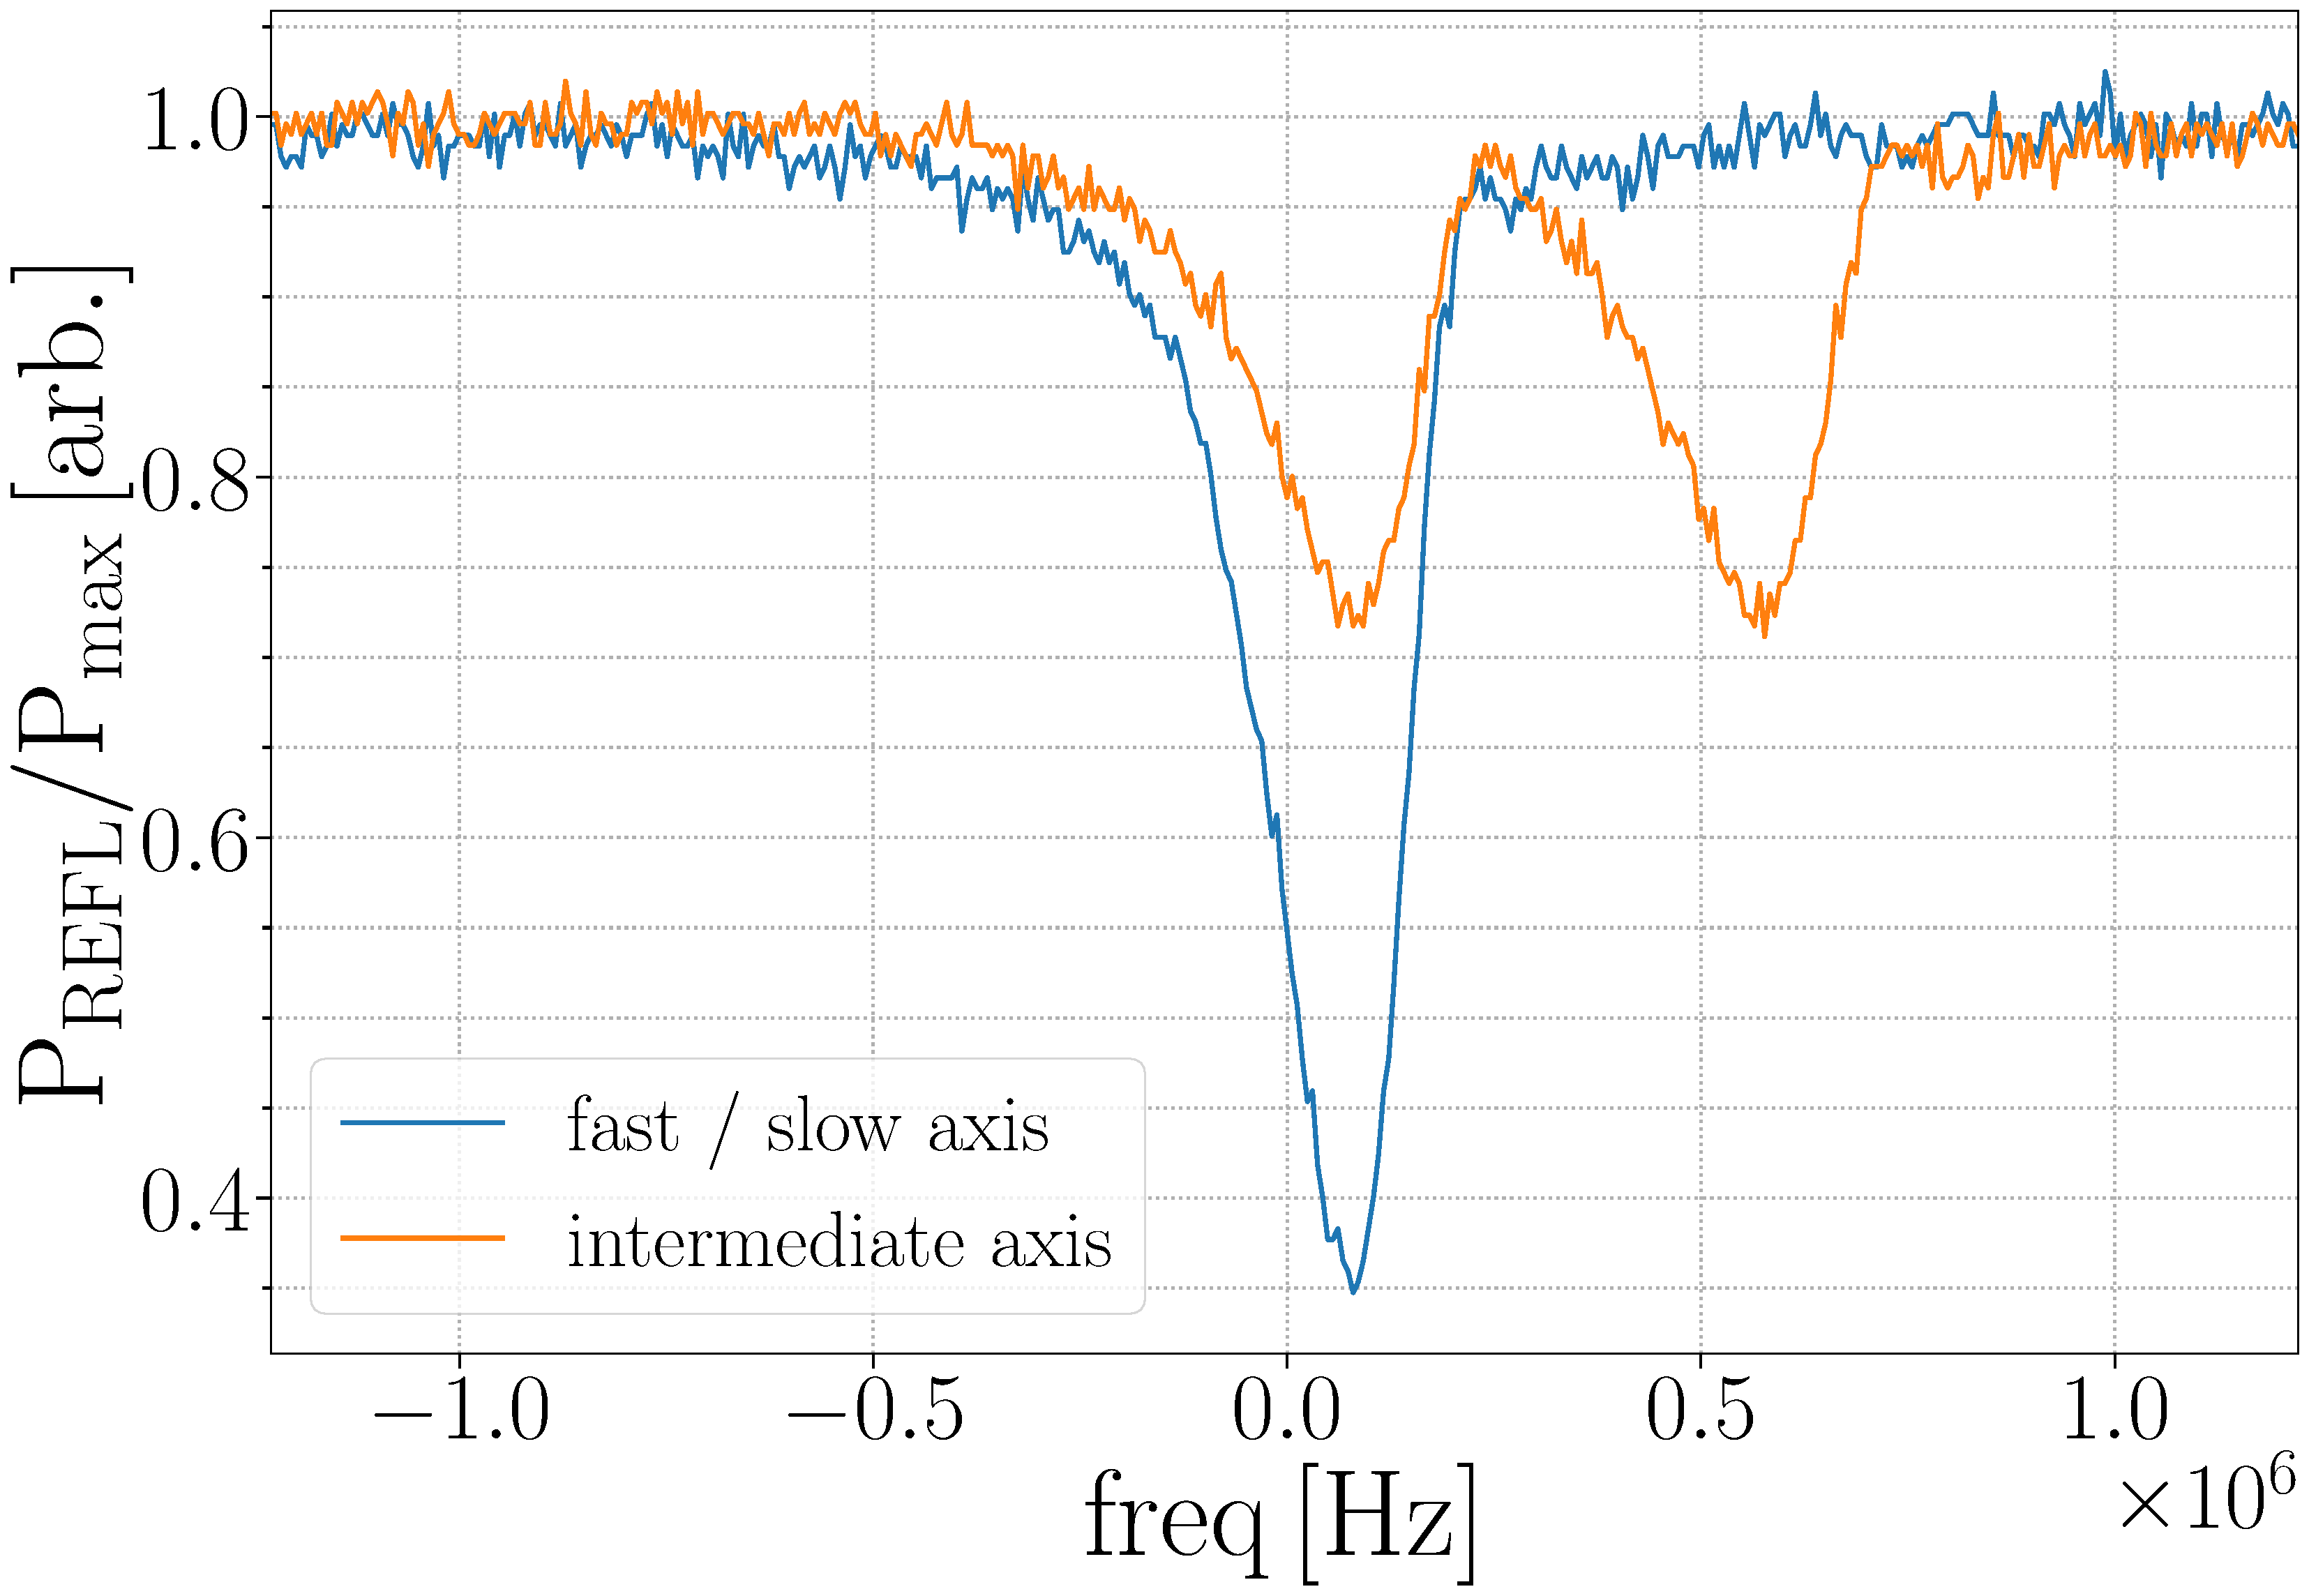
\includegraphics[width=\linewidth]{figs/ALGAAS/split_cav_scan.pdf}
	\label{splitresonance}
    \end{subfigure}
    \begin{subfigure}{.50\linewidth}
	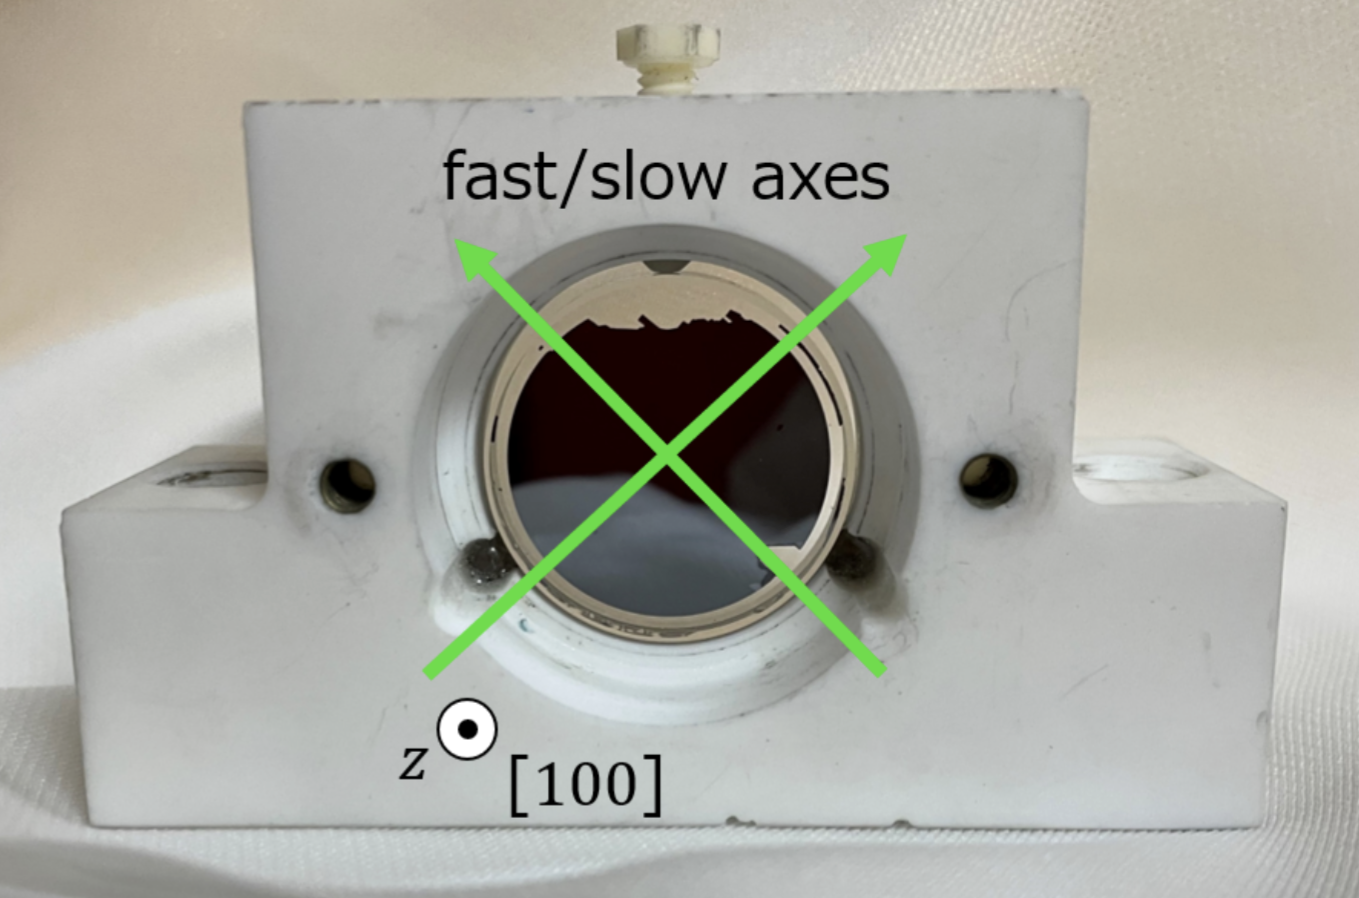
\includegraphics[width=\linewidth]{figs/ALGAAS/fas_axes.png}
	\label{fast_slow_axes}
    \end{subfigure}
    \caption{[Right] Lines running parallel to fast and slow axes. It was understood prior that a flat would be normal to one of the two eigenaxes. Measurement of the split resonance [Left] suggests no flat to be present and the damage seen is due to excessive handling. This split has the indicated frequency separation of 500 kHz.}
    \label{fig:split_cav_resonance}
\end{figure}

\begin{figure}[!h]
    \centering
    \begin{subcaptiongroup}
	    \includegraphics[page=2,width=.325\textwidth]{ALGAAS/laser_mirror_algaas_coat_defect.pdf}
	    \phantomcaption\label{conormaldefect}
	    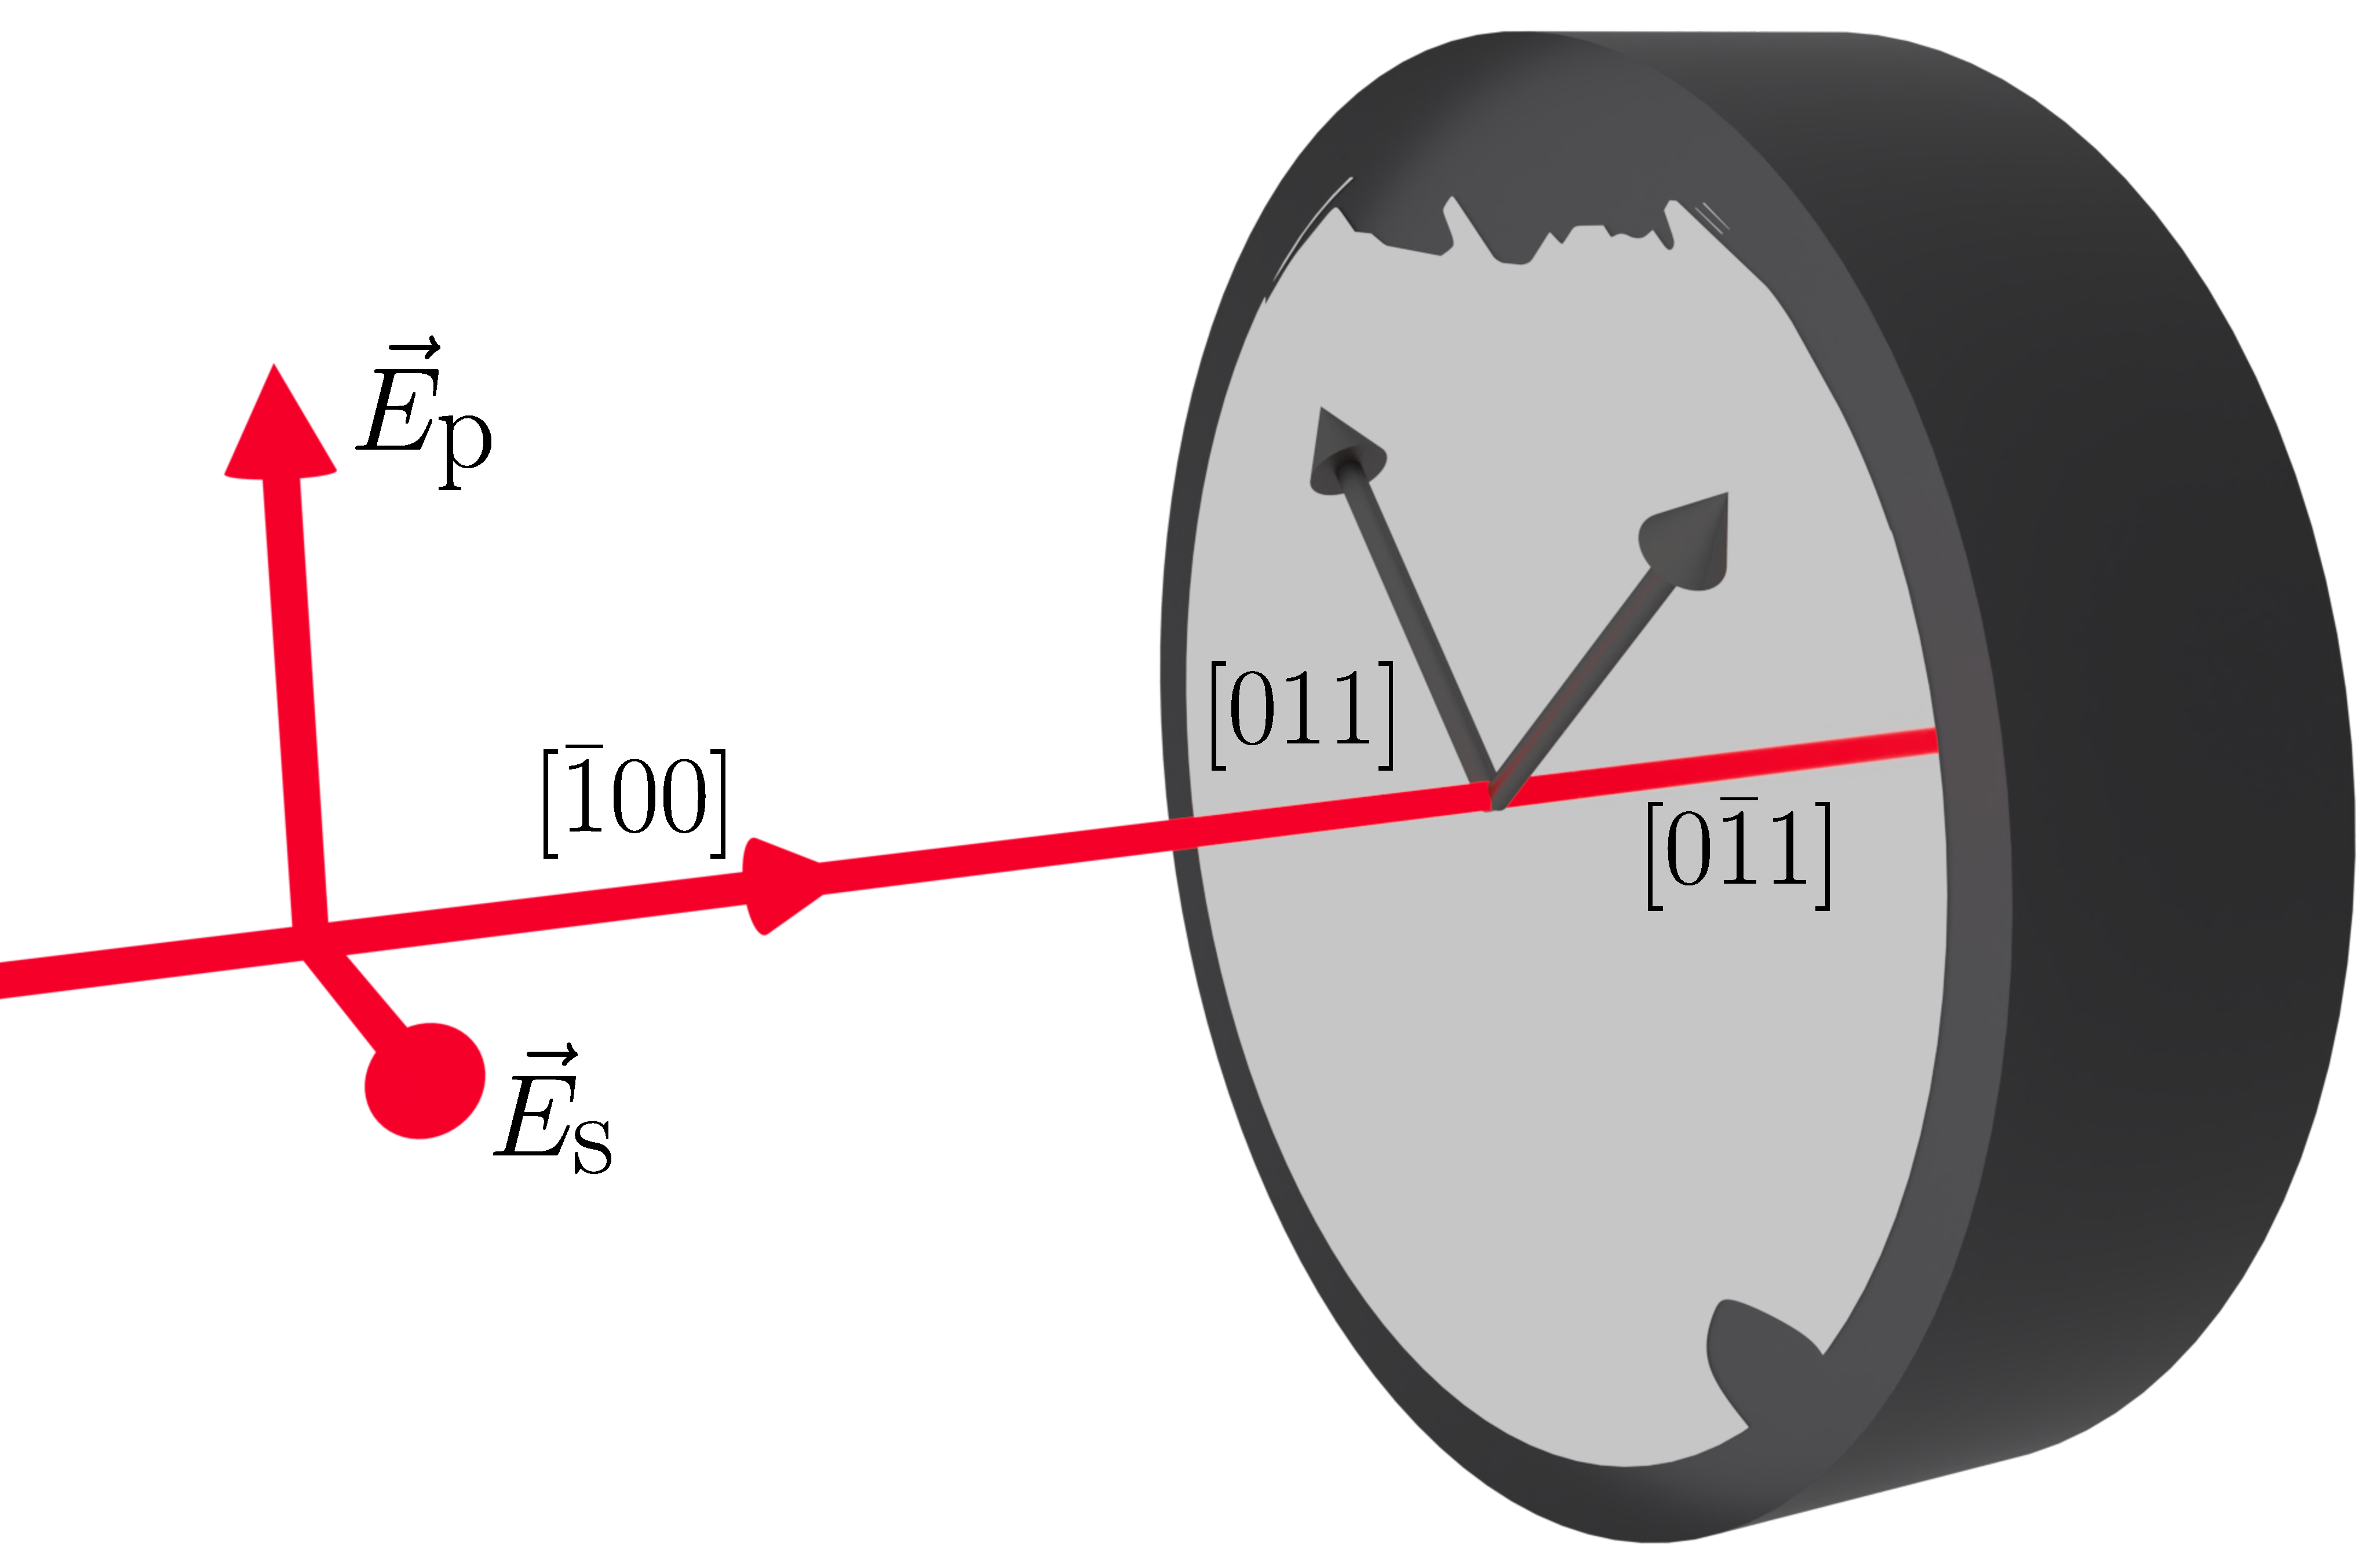
\includegraphics[page=1,width=.5\textwidth]{ALGAAS/laser_mirror_algaas_coat_defect.pdf}
	    \phantomcaption\label{coisodefect}
    \end{subcaptiongroup}
    \caption{Input beam orientation with respect to the coating miller indices / fast and slow axes, with a [Left] Normal view and [Right] isometric view.}
\end{figure}


%There are different accounts of a measured birefringence from HR $\gaas$ / $\algaas$ coatings (\href{https://dcc.ligo.org/DocDB/0181/G2200386/001/G2200386.pdf}{Satoshi}, \href{https://nodus.ligo.caltech.edu:8081/CTN/1474}{CTN}, \href{https://dcc.ligo.org/DocDB/0181/G2200559/001/G2200559-v1\%20-\%20polarization.pdf}{Aidan})
%%Is the measured birefringence static? (Layer bonding method might introduce something?)
%% Does it change from different mounting methods? (Photoelastic) (order of magnitude estimate)
%% Electro-optic ruled out based on field measurements and relative coupling factor.
%% Measurement precision of the coating birefringence? Cavity length, Polarization drifts, etc.
From coating manufacturers it's estimated that static birefringence can arise from the intrinsic strain between hetero-epitaxial layers of $\gaas$/$\algaas$. \cite{cole:2013, adachi:1985}

\section{Results}
\subsection{Acousto-optical noise}
A significant barrier to low differential length noise sensitivity for this experiment is the lack of low-noise optical mounts in accessible non-conductive materials. Most commercial optical mounts are constructed with conductive materials which proves problematic when seeking to isolate the coating from non-normal field gradients within the coating volume of interest. For this reason, there were multiple efforts were focused on developing a suitable mounting solution that would provide adequate isolation from any uncontrolled field magnitudes while driving a field normally incident on the surface with enough strength and uniformity across the beam area to extract a measurement of the differential length change from the Pockels effect. Varying the mechanical configurations (i.e. differential electrode and / or optic set screw settings) to the slightest degree left us to discover a variety of drive couplings via excitations from the assembly sample-mount acoustic modes driving the voltage on electrodes plates. Tracking consistent mechanical response for assemblies prior to Assembly 3 proved challenging due to inconsistent mechanical settings between some measurements and span different geometries / material properties \footnote{For more details see \autoref{appendix:mount_assemblies}}. An adequate solution was dependent on selecting a material and geometry that would generate narrow acoustic resonances while simultaneously achieving adequately low noise within a bandwidth of interest (a not so uncommon experimental principle that is heavily used and mentioned within collaboration literature). The associated configuration \footnote{Assembly 3 : \autoref{fig:assembly3}} provided such a solution and the driven acoustic modes (\textless 10 kHz \& 40kHz - 80kHz) were confirmed when comparing the cavity response between $\gaas$/$\algaas$ coating and the non-crystalline HR coating from ATFilms \footnote{A null measurement reference} with additional confirmation from finite element analysis.  From here, an upper threshold noise estimate of the electro-optic coupling is extracted by taking the difference between fast and slow axes:


\[ 
    \begin{aligned}
	\mathrm{diff} & = C_\mathrm{slow} - C_\mathrm{fast} \\
		      & = (C_\mathrm{m, slow} + C_\mathrm{EO, slow}) - (C_\mathrm{m, fast} + C_\mathrm{EO, fast}) \\
		      & =  2 |C_\mathrm{EO}| e^{i \psi}
    \end{aligned}
\]

\subsection{EO coupling estimate}

\begin{figure}[H]
    \centering
    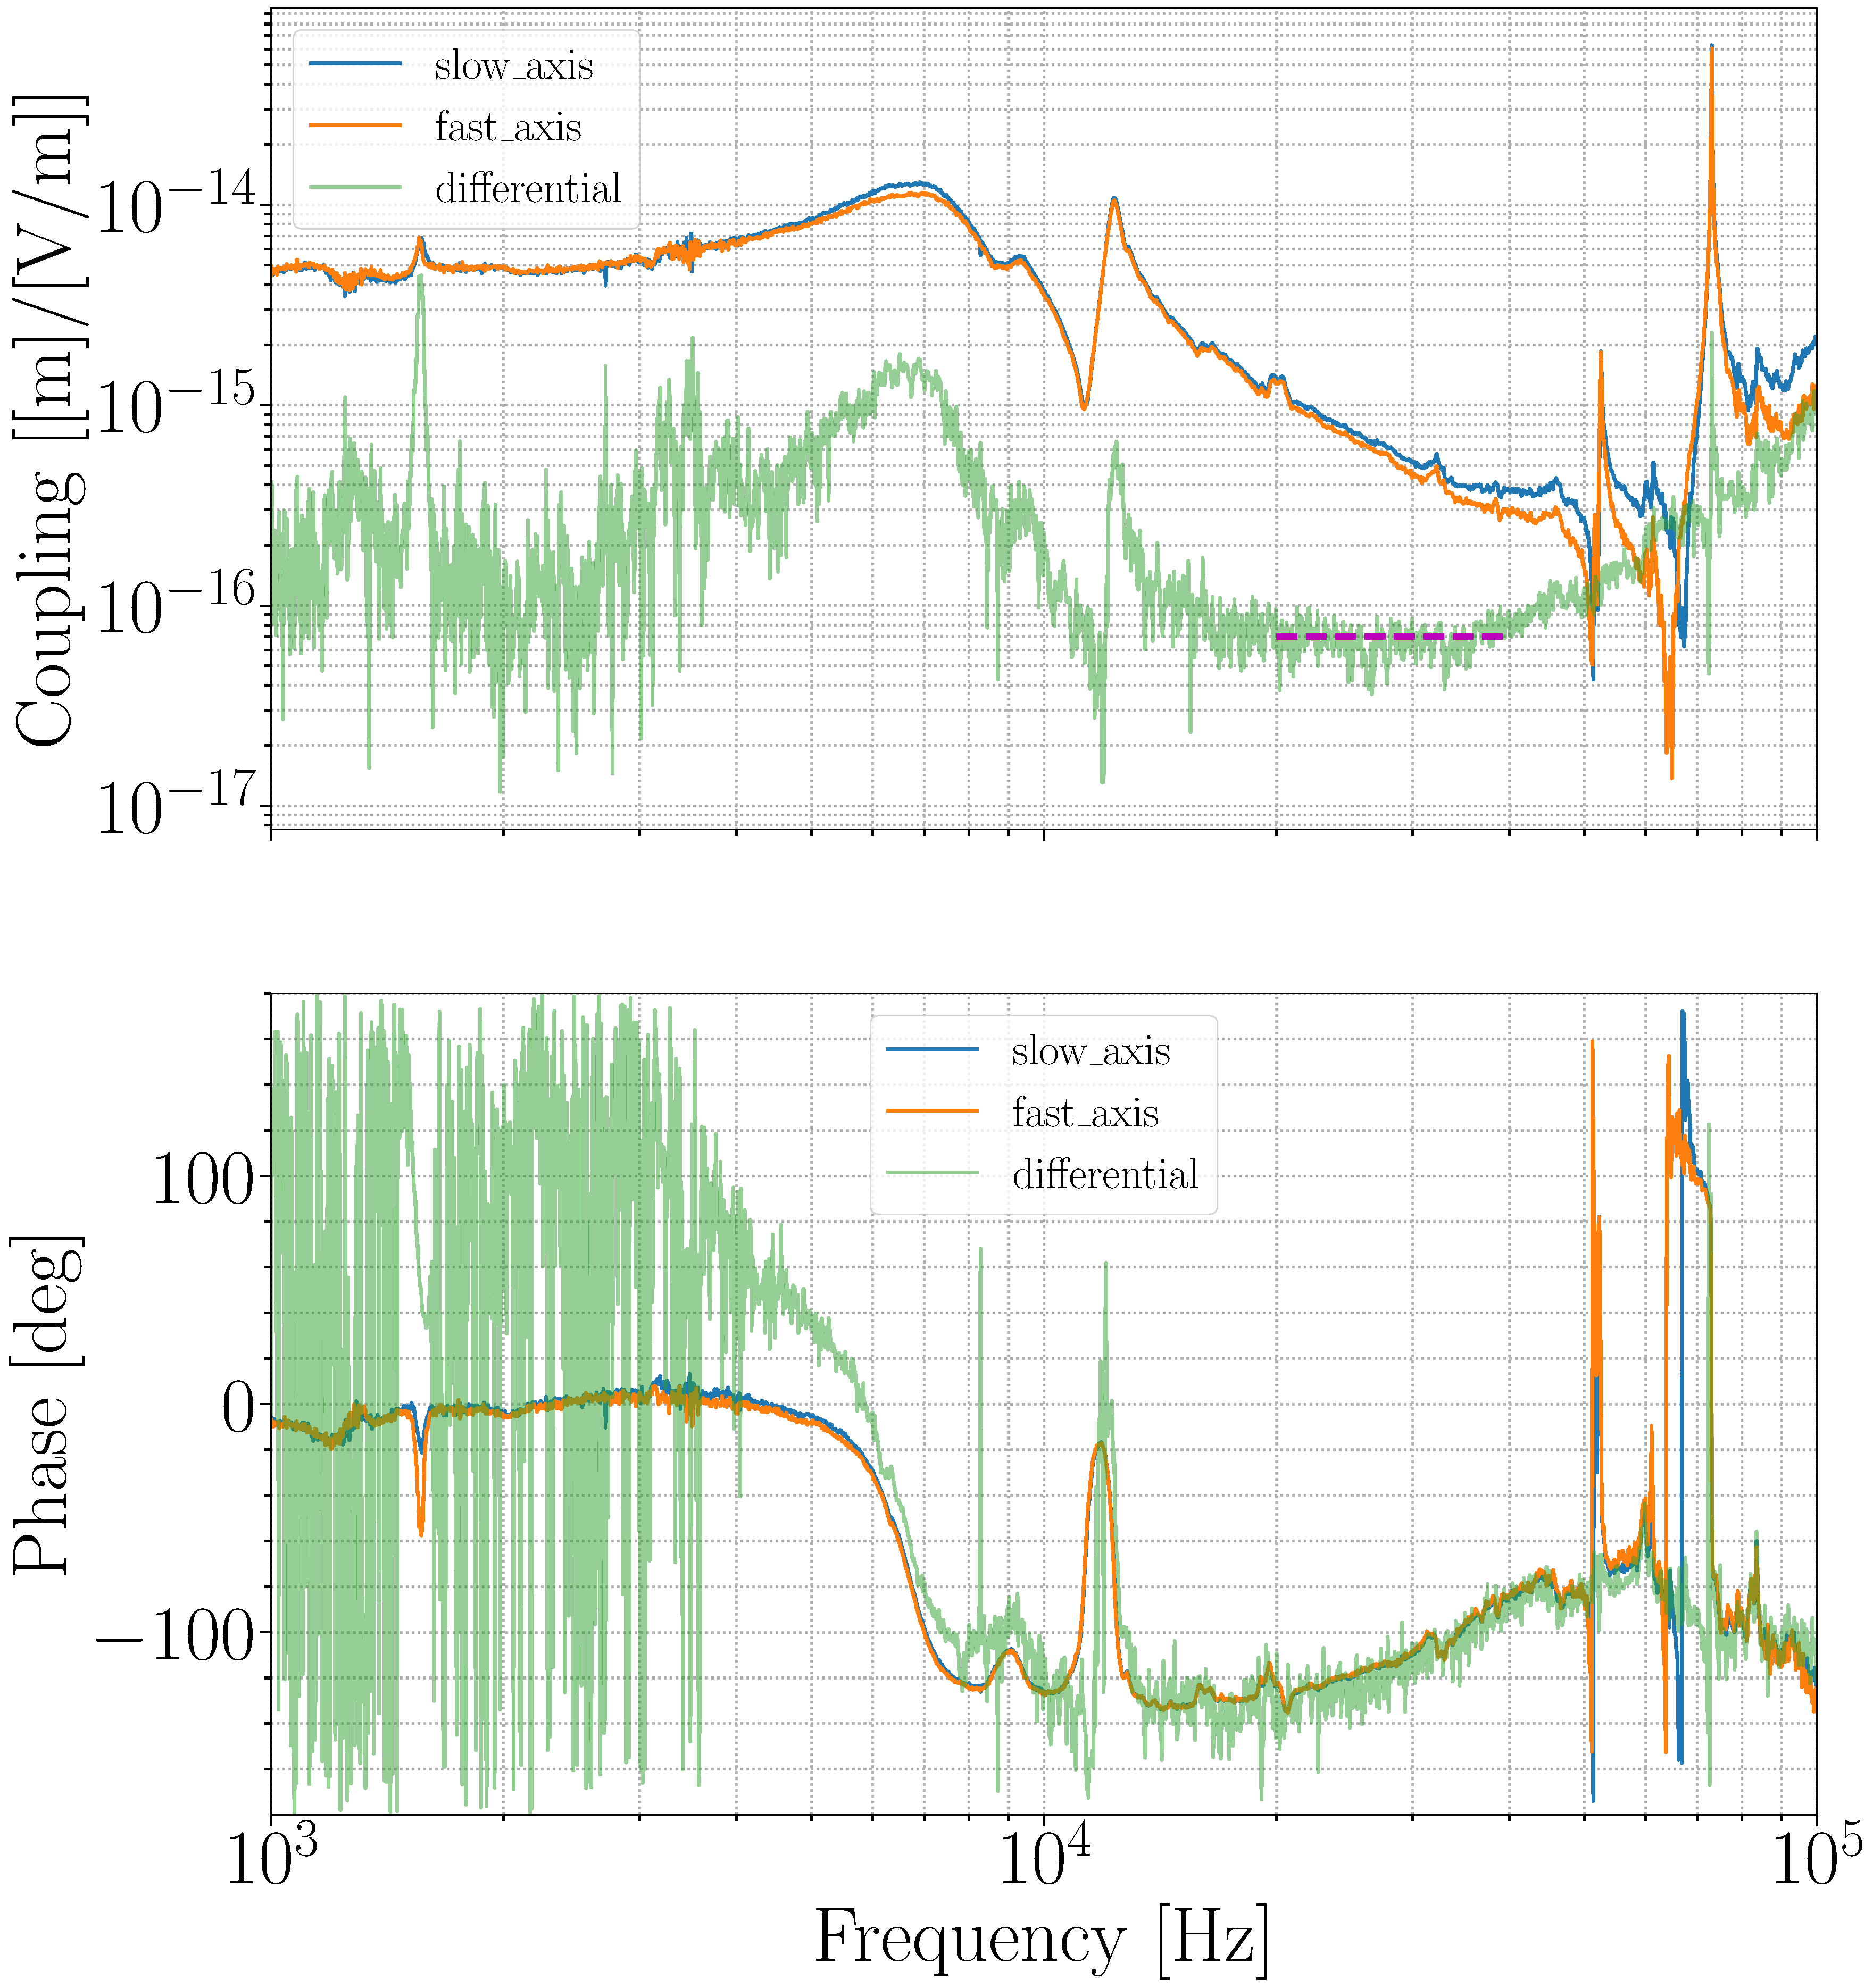
\includegraphics[width=.91\textwidth]{figs/ALGAAS/coupling_tf.pdf}
    \caption{Calibrated measurement of the conversion factor of field strength [V/m] to length [m] when the beam input polarization is aligned along the slow and fast $\gaas$ / $\algaas$ coating axes.}
    \label{fig:final_tf_conversion}
\end{figure}


From this experiment an upper threshold estimate between 20 kHz - 40 kHz is $\approx \; 6.5 \times 10^{-17} \; [\mathrm{m}]/[\mathrm{V}/\mathrm{m}]$ \iffalse $\approx \; 1.1 \times 10^{-17} \; [\mathrm{m}]/[\mathrm{V}/\mathrm{m}]$ \fi though at higher frequency, frequency dispersion of the electro-optic coefficients may explain the increase.  The uniform flat response is extended to frequencies at which LIGO operates 10 Hz - 1 kHz as prior work has demonstrated such a trend from 10 Hz to several 10s of kHz ~\cite{salvestrini:2003}.

The significantly improved thermal noise performance of $\gaas$/$\algaas$ HR coatings make these crystalline coatings a prime candidate for the core optics in current and future gravitational wave detectors. The measured upper threshold of the electro-optic noise is demonstrated to be $\sim 10^{-26} \; [1/\sqrt{\mathrm{Hz}}]$ two orders of magnitude below the designed noise floor $\sim 10^{-24}\; [1/\sqrt{\mathrm{Hz}}]$ of current and future gravitational wave detectors.

%\begin{itemize}
%\item \textbf{Vibration of plates (Leissa)} \cite{leissa:1969} Computing frequencies and order of magnitude
%	\begin{itemize}
%	    \item Numerical computation (Order of magnitude result)
%	\end{itemize}
%\item \textbf{Steve's COMSOL model results}
%\end{itemize}
\fi
